% Options for packages loaded elsewhere
\PassOptionsToPackage{unicode}{hyperref}
\PassOptionsToPackage{hyphens}{url}
%
\documentclass[
]{article}
\usepackage{lmodern}
\usepackage{amssymb,amsmath}
\usepackage{ifxetex,ifluatex}
\ifnum 0\ifxetex 1\fi\ifluatex 1\fi=0 % if pdftex
  \usepackage[T1]{fontenc}
  \usepackage[utf8]{inputenc}
  \usepackage{textcomp} % provide euro and other symbols
\else % if luatex or xetex
  \usepackage{unicode-math}
  \defaultfontfeatures{Scale=MatchLowercase}
  \defaultfontfeatures[\rmfamily]{Ligatures=TeX,Scale=1}
\fi
% Use upquote if available, for straight quotes in verbatim environments
\IfFileExists{upquote.sty}{\usepackage{upquote}}{}
\IfFileExists{microtype.sty}{% use microtype if available
  \usepackage[]{microtype}
  \UseMicrotypeSet[protrusion]{basicmath} % disable protrusion for tt fonts
}{}
\makeatletter
\@ifundefined{KOMAClassName}{% if non-KOMA class
  \IfFileExists{parskip.sty}{%
    \usepackage{parskip}
  }{% else
    \setlength{\parindent}{0pt}
    \setlength{\parskip}{6pt plus 2pt minus 1pt}}
}{% if KOMA class
  \KOMAoptions{parskip=half}}
\makeatother
\usepackage{xcolor}
\IfFileExists{xurl.sty}{\usepackage{xurl}}{} % add URL line breaks if available
\IfFileExists{bookmark.sty}{\usepackage{bookmark}}{\usepackage{hyperref}}
\hypersetup{
  pdftitle={Agerage User},
  pdfauthor={Ariella Fuzaylov},
  hidelinks,
  pdfcreator={LaTeX via pandoc}}
\urlstyle{same} % disable monospaced font for URLs
\usepackage[margin=1in]{geometry}
\usepackage{color}
\usepackage{fancyvrb}
\newcommand{\VerbBar}{|}
\newcommand{\VERB}{\Verb[commandchars=\\\{\}]}
\DefineVerbatimEnvironment{Highlighting}{Verbatim}{commandchars=\\\{\}}
% Add ',fontsize=\small' for more characters per line
\usepackage{framed}
\definecolor{shadecolor}{RGB}{248,248,248}
\newenvironment{Shaded}{\begin{snugshade}}{\end{snugshade}}
\newcommand{\AlertTok}[1]{\textcolor[rgb]{0.94,0.16,0.16}{#1}}
\newcommand{\AnnotationTok}[1]{\textcolor[rgb]{0.56,0.35,0.01}{\textbf{\textit{#1}}}}
\newcommand{\AttributeTok}[1]{\textcolor[rgb]{0.77,0.63,0.00}{#1}}
\newcommand{\BaseNTok}[1]{\textcolor[rgb]{0.00,0.00,0.81}{#1}}
\newcommand{\BuiltInTok}[1]{#1}
\newcommand{\CharTok}[1]{\textcolor[rgb]{0.31,0.60,0.02}{#1}}
\newcommand{\CommentTok}[1]{\textcolor[rgb]{0.56,0.35,0.01}{\textit{#1}}}
\newcommand{\CommentVarTok}[1]{\textcolor[rgb]{0.56,0.35,0.01}{\textbf{\textit{#1}}}}
\newcommand{\ConstantTok}[1]{\textcolor[rgb]{0.00,0.00,0.00}{#1}}
\newcommand{\ControlFlowTok}[1]{\textcolor[rgb]{0.13,0.29,0.53}{\textbf{#1}}}
\newcommand{\DataTypeTok}[1]{\textcolor[rgb]{0.13,0.29,0.53}{#1}}
\newcommand{\DecValTok}[1]{\textcolor[rgb]{0.00,0.00,0.81}{#1}}
\newcommand{\DocumentationTok}[1]{\textcolor[rgb]{0.56,0.35,0.01}{\textbf{\textit{#1}}}}
\newcommand{\ErrorTok}[1]{\textcolor[rgb]{0.64,0.00,0.00}{\textbf{#1}}}
\newcommand{\ExtensionTok}[1]{#1}
\newcommand{\FloatTok}[1]{\textcolor[rgb]{0.00,0.00,0.81}{#1}}
\newcommand{\FunctionTok}[1]{\textcolor[rgb]{0.00,0.00,0.00}{#1}}
\newcommand{\ImportTok}[1]{#1}
\newcommand{\InformationTok}[1]{\textcolor[rgb]{0.56,0.35,0.01}{\textbf{\textit{#1}}}}
\newcommand{\KeywordTok}[1]{\textcolor[rgb]{0.13,0.29,0.53}{\textbf{#1}}}
\newcommand{\NormalTok}[1]{#1}
\newcommand{\OperatorTok}[1]{\textcolor[rgb]{0.81,0.36,0.00}{\textbf{#1}}}
\newcommand{\OtherTok}[1]{\textcolor[rgb]{0.56,0.35,0.01}{#1}}
\newcommand{\PreprocessorTok}[1]{\textcolor[rgb]{0.56,0.35,0.01}{\textit{#1}}}
\newcommand{\RegionMarkerTok}[1]{#1}
\newcommand{\SpecialCharTok}[1]{\textcolor[rgb]{0.00,0.00,0.00}{#1}}
\newcommand{\SpecialStringTok}[1]{\textcolor[rgb]{0.31,0.60,0.02}{#1}}
\newcommand{\StringTok}[1]{\textcolor[rgb]{0.31,0.60,0.02}{#1}}
\newcommand{\VariableTok}[1]{\textcolor[rgb]{0.00,0.00,0.00}{#1}}
\newcommand{\VerbatimStringTok}[1]{\textcolor[rgb]{0.31,0.60,0.02}{#1}}
\newcommand{\WarningTok}[1]{\textcolor[rgb]{0.56,0.35,0.01}{\textbf{\textit{#1}}}}
\usepackage{graphicx,grffile}
\makeatletter
\def\maxwidth{\ifdim\Gin@nat@width>\linewidth\linewidth\else\Gin@nat@width\fi}
\def\maxheight{\ifdim\Gin@nat@height>\textheight\textheight\else\Gin@nat@height\fi}
\makeatother
% Scale images if necessary, so that they will not overflow the page
% margins by default, and it is still possible to overwrite the defaults
% using explicit options in \includegraphics[width, height, ...]{}
\setkeys{Gin}{width=\maxwidth,height=\maxheight,keepaspectratio}
% Set default figure placement to htbp
\makeatletter
\def\fps@figure{htbp}
\makeatother
\setlength{\emergencystretch}{3em} % prevent overfull lines
\providecommand{\tightlist}{%
  \setlength{\itemsep}{0pt}\setlength{\parskip}{0pt}}
\setcounter{secnumdepth}{-\maxdimen} % remove section numbering

\title{Agerage User}
\author{Ariella Fuzaylov}
\date{3/23/2021}

\begin{document}
\maketitle

\hypertarget{loading-data-from-csv-and-update-header}{%
\subsection{Loading Data From CSV and Update
Header}\label{loading-data-from-csv-and-update-header}}

\begin{Shaded}
\begin{Highlighting}[]
\NormalTok{my.data=}\KeywordTok{read.csv}\NormalTok{(}\StringTok{"Online Recipe Sharing.csv"}\NormalTok{, }\DataTypeTok{header=}\OtherTok{TRUE}\NormalTok{)}
\KeywordTok{colnames}\NormalTok{(my.data)}
\end{Highlighting}
\end{Shaded}

\begin{verbatim}
##  [1] "Timestamp"                                                                                                                                                                                                 
##  [2] "What.is.your.age."                                                                                                                                                                                         
##  [3] "Who.is.the.usual.meal.prepper.in.your.household."                                                                                                                                                          
##  [4] "Do.you..or.any.household.member.you.share.meals.with..have.any.dietary.restrictions."                                                                                                                      
##  [5] "How.often.do.you.eat.food.prepared.at.home."                                                                                                                                                               
##  [6] "When.you.are.cooking.using.a.recipe..what.format.do.you.view.the.recipe.in..Select.all.that.apply"                                                                                                         
##  [7] "When.you.are.looking.for.a.recipe..what.websites.do.you.visit.the.most.."                                                                                                                                  
##  [8] "Which.website.do.you.enjoy.using.for.finding.recipes."                                                                                                                                                     
##  [9] "Optional..Explain.what.you.like.about.these.websites."                                                                                                                                                     
## [10] "Which.website.do.you.NOT.enjoy.using.for.finding.recipes."                                                                                                                                                 
## [11] "Optional..Explain.what.you.dislike.about.these.websites."                                                                                                                                                  
## [12] "When.deciding.what.to.cook..how.often.do.you.search.for.a.specific.recipe.in.the.search.bar.provided.by.your.website.of.choice."                                                                           
## [13] "How.often.do.you.use.the.search.bar.to.find.a.recipe.you.have.used.in.the.past."                                                                                                                           
## [14] "When.deciding.on.a.dish.to.prepare..how.often.do.you.browse.available.articles.or.recipe.collections.for.inspiration.on.what.to.cook."                                                                     
## [15] "When.deciding.what.to.cook..how.many.recipes.do.you.typically.click.on.before.you.find.a.suitable.recipe."                                                                                                 
## [16] "Do.the.websites.you.visit.when.looking.for.inspiration.on.what.to.cook.differ.from.the.websites.you.use.to.find.specific.recipes...i.e.looking.for.Mexican.food.instead.of.specifically.a.carnitas.recipe."
## [17] "When.you.are.looking.for.cooking.inspiration..what.websites.do.you.visit.the.most.."                                                                                                                       
## [18] "Which.websites.do.you.enjoy.using.when.looking.for.cooking.inspiration."                                                                                                                                   
## [19] "Optional..Explain.what.you.like.about.these.websites..1"                                                                                                                                                   
## [20] "Which.websites.do.you.NOT.enjoy.using.when.looking.for.cooking.inspiration."                                                                                                                               
## [21] "Optional..Explain.what.you.dislike.about.these.websites..1"                                                                                                                                                
## [22] "When.looking.for.recipe.recommendations.or.reviews.where.do.you.look..Select.all.that.apply"                                                                                                               
## [23] "What.source.of.recommendations.or.reviews.is.most.likely.to.influence.your.recipe.choice..Select.all.that.apply"                                                                                           
## [24] "How.often.do.you.try.a.new.recipe.based.on.a.recommendation.or.review.from.a.trusted.source."                                                                                                              
## [25] "How.often.do.you.seek.out.a.recipe.recommendation.or.review.from.a.trusted.source."                                                                                                                        
## [26] "How.often.do.you.recommend.or.review.a.recipe.you.have.made."                                                                                                                                              
## [27] "How.often.do.you.save.a.recipe.to.use.later."                                                                                                                                                              
## [28] "When.saving.recipes.to.use.later..what.tools.do.you.use."                                                                                                                                                  
## [29] "How.often.do.you.make.a.recipe.exactly.as.written..As.opposed.to.finding.a.recipe.that.exactly.matches.your.needs."                                                                                        
## [30] "If.you.make.modifications.to.a.recipe.what.factors.influence.your.modifications..Select.all.that.apply"                                                                                                    
## [31] "How.often.do.you.take.note.of.a.modification.you.have.made.to.a.recipe."                                                                                                                                   
## [32] "How.do.you.take.note.of.modifications.you.have.made.to.a.recipe."                                                                                                                                          
## [33] "Are.you.satisfied.with.the.available.options.for.recording.recipe.notes."                                                                                                                                  
## [34] "Would.you.like.to.take.digital.notes.given.better.note.taking.options."                                                                                                                                    
## [35] "How.often.do.you.discuss.a.recipe.you.have.made."                                                                                                                                                          
## [36] "How.often.do.you.read.the.discussion.of.a.recipe."                                                                                                                                                         
## [37] "What.medium.do.you.primarily.use.to.discuss.recipes."                                                                                                                                                      
## [38] "What.do.you.like.most.about.the.discussion.platforms.you.use."                                                                                                                                             
## [39] "Just.looking.at.the.layout..choose.the.option.you.like.the.most."                                                                                                                                          
## [40] "Just.looking.at.the.layout..choose.the.option.you.like.the.most..1"                                                                                                                                        
## [41] "Just.looking.at.the.layout..choose.the.option.you.like.the.most..2"                                                                                                                                        
## [42] "Just.looking.at.the.layout..choose.the.option.you.like.the.most..3"                                                                                                                                        
## [43] "Just.looking.at.the.layout..choose.the.option.you.like.the.most..4"                                                                                                                                        
## [44] "Just.looking.at.the.layout..choose.the.option.you.like.the.most..5"
\end{verbatim}

\begin{Shaded}
\begin{Highlighting}[]
\KeywordTok{colnames}\NormalTok{(my.data)<-}\KeywordTok{c}\NormalTok{(}\StringTok{"Timestamp"}\NormalTok{, }\StringTok{"Age"}\NormalTok{, }\StringTok{"Primary.Meal.Prepper"}\NormalTok{, }\StringTok{"Household.Dietary.Restriction"}\NormalTok{,}
\StringTok{"Home.Cooking.Rate"}\NormalTok{, }
\StringTok{"Primary.Recipe.Format"}\NormalTok{, }
\StringTok{"Primary.Search.Website"}\NormalTok{,}
\StringTok{"Enjoyed.Website.Searching"}\NormalTok{, }\StringTok{"Comments.Enjoyed.Website.Searching"}\NormalTok{, }\StringTok{"NOT.Enjoyed.Website.Searching"}\NormalTok{, }\StringTok{"Comments.NOT.Enjoyed.Website.Searching"}\NormalTok{, }\StringTok{"Recipe.Search.Bar.Frequency"}\NormalTok{, }
\StringTok{"Previous.Recipe.Search.Frequency"}\NormalTok{,}
\StringTok{"Browsing.While.Searching.Frequecny"}\NormalTok{, }
\StringTok{"Click.Rate"}\NormalTok{, }
\StringTok{"Search.Browse.Same.Websites"}\NormalTok{,}
\StringTok{"Primary.Browsing.Website"}\NormalTok{, }
\StringTok{"Enjoyed.Website.Browsing"}\NormalTok{, }
\StringTok{"Comments.Enjoyed.Website.Browsing"}\NormalTok{, }\StringTok{"NOT.Enjoyed.Website.Browsing"}\NormalTok{, }\StringTok{"Comments.NOT.Enjoyed.Website.Browsing"}\NormalTok{, }\StringTok{"Primary.Source.of.Reviews"}\NormalTok{,}
\StringTok{"Source.of.Influential.Reviews"}\NormalTok{, }\StringTok{"Frequency.Reviews.Effect.Behavior"}\NormalTok{, }
\StringTok{"Frequency.Seek.Out.Review"}\NormalTok{, }
\StringTok{"Frequency.of.Review"}\NormalTok{, }
\StringTok{"Frequency.of.Recipe.Saving"}\NormalTok{, }
\StringTok{"Method.of.Recipe.Saving"}\NormalTok{, }
\StringTok{"Modification.Frequency"}\NormalTok{, }
\StringTok{"Modification.Influence.Factors"}\NormalTok{,}
\StringTok{"Modification.Record.Frequency"}\NormalTok{, }
\StringTok{"Modification.Record.Method"}\NormalTok{, }
\StringTok{"Satisfaction.with.Available.Record.Methods"}\NormalTok{, }
\StringTok{"Interest.in.Improved.Record.Method"}\NormalTok{,}
\StringTok{"Frequency.of.Recipe.Discussion"}\NormalTok{, }\StringTok{"Frequency.of.Reading.Discussion"}\NormalTok{,}
\StringTok{"Primary.Discussion.Medium"}\NormalTok{, }\StringTok{"Enjoyed.Features.of.Discussion.Mediums"}\NormalTok{, }\StringTok{"Ingredients.L.V.Above"}\NormalTok{, }
\StringTok{"Ingredients.L.Comments.Inline.V.Below"}\NormalTok{, }\StringTok{"Ingredients.Above.Comments.Below.V.Inline"}\NormalTok{, }\StringTok{"Ingredients.By.Step.V.Above"}\NormalTok{, }
\StringTok{"Ingredients.By.Step.V.Scroll.L"}\NormalTok{, }
\StringTok{"Ingredients.Above.V.Scroll.L"}\NormalTok{)}
\end{Highlighting}
\end{Shaded}

\hypertarget{re-factor-data}{%
\subsection{Re-Factor Data}\label{re-factor-data}}

If Respondent indicated that they search and browse on the same
websites, populate the empty cells with the same data. This assumes that
the user's searching behavior is exactly the same as the browsing
behavior if the user selected yes for searching and browsing on the same
websites.

\begin{Shaded}
\begin{Highlighting}[]
\ControlFlowTok{for}\NormalTok{ (i }\ControlFlowTok{in} \DecValTok{1}\OperatorTok{:}\KeywordTok{nrow}\NormalTok{(my.data))\{}
  \ControlFlowTok{if}\NormalTok{ (my.data}\OperatorTok{$}\NormalTok{Search.Browse.Same.Websites[i]}\OperatorTok{==}\StringTok{"No"}\NormalTok{)\{}
\NormalTok{    my.data}\OperatorTok{$}\NormalTok{Primary.Browsing.Website[i]<-my.data}\OperatorTok{$}\NormalTok{Primary.Search.Website[i]}
\NormalTok{    my.data}\OperatorTok{$}\NormalTok{Enjoyed.Website.Browsing[i]<-my.data}\OperatorTok{$}\NormalTok{Enjoyed.Website.Searching[i]}
\NormalTok{    my.data}\OperatorTok{$}\NormalTok{NOT.Enjoyed.Website.Browsing[i]<-my.data}\OperatorTok{$}\NormalTok{NOT.Enjoyed.Website.Searching[i]}
\NormalTok{  \}}
\NormalTok{\}}
\end{Highlighting}
\end{Shaded}

Since the data set is small, I am consolidating some of the categories.

\begin{itemize}
\item
  Primary Meal Prepper will be Respondent if the individual taking the
  survey indicated that they are the primary meal prepper in their
  household or if they cook for themselves, and other in all other
  cases.
\item
  Dietary restriction will become a yes or no question
\item
  Home Cooking Rate will become Daily if the respondents cooks at home
  most days, weekly if the respondent cooks several times a week, and
  monthly is the respondent cooks a couple times a month.
\end{itemize}

\begin{Shaded}
\begin{Highlighting}[]
\NormalTok{my.data.factored<-my.data}
\NormalTok{my.data.factored}\OperatorTok{$}\NormalTok{Age<-}\KeywordTok{as.factor}\NormalTok{(my.data}\OperatorTok{$}\NormalTok{Age)}

\NormalTok{my.data.factored}\OperatorTok{$}\NormalTok{Primary.Meal.Prepper<-}\KeywordTok{as.factor}\NormalTok{(my.data.factored}\OperatorTok{$}\NormalTok{Primary.Meal.Prepper)}

\NormalTok{my.data.factored}\OperatorTok{$}\NormalTok{Household.Dietary.Restriction<-}\KeywordTok{as.factor}\NormalTok{(my.data.factored}\OperatorTok{$}\NormalTok{Household.Dietary.Restriction)}

\NormalTok{my.data.factored}\OperatorTok{$}\NormalTok{Home.Cooking.Rate<-}\KeywordTok{as.factor}\NormalTok{(my.data.factored}\OperatorTok{$}\NormalTok{Home.Cooking.Rate)}

\NormalTok{my.data.factored}\OperatorTok{$}\NormalTok{Ingredients.L.V.Above<-}\KeywordTok{as.factor}\NormalTok{(my.data.factored}\OperatorTok{$}\NormalTok{Ingredients.L.V.Above)}
\NormalTok{my.data.factored}\OperatorTok{$}\NormalTok{Ingredients.By.Step.V.Above<-}\KeywordTok{as.factor}\NormalTok{(my.data.factored}\OperatorTok{$}\NormalTok{Ingredients.By.Step.V.Above)}
\NormalTok{my.data.factored}\OperatorTok{$}\NormalTok{Ingredients.Above.V.Scroll.L<-}\KeywordTok{as.factor}\NormalTok{(my.data.factored}\OperatorTok{$}\NormalTok{Ingredients.Above.V.Scroll.L)}
\NormalTok{my.data.factored}\OperatorTok{$}\NormalTok{Ingredients.L.Comments.Inline.V.Below<-}\KeywordTok{as.factor}\NormalTok{(my.data.factored}\OperatorTok{$}\NormalTok{Ingredients.L.Comments.Inline.V.Below)}
\NormalTok{my.data.factored}\OperatorTok{$}\NormalTok{Ingredients.By.Step.V.Scroll.L<-}
\StringTok{  }\KeywordTok{as.factor}\NormalTok{(my.data.factored}\OperatorTok{$}\NormalTok{Ingredients.By.Step.V.Scroll.L)}
\NormalTok{my.data.factored}\OperatorTok{$}\NormalTok{Ingredients.Above.Comments.Below.V.Inline<-}
\StringTok{  }\KeywordTok{as.factor}\NormalTok{(my.data.factored}\OperatorTok{$}\NormalTok{Ingredients.Above.Comments.Below.V.Inline)}
\NormalTok{my.data.factored<-}\StringTok{ }\KeywordTok{mutate}\NormalTok{(my.data.factored, }
                          \DataTypeTok{Age =} \KeywordTok{fct_collapse}\NormalTok{(Age, }
                                             \DataTypeTok{YA =} \KeywordTok{c}\NormalTok{(}\StringTok{"18 - 24 years old"}\NormalTok{,}\StringTok{"25 - 34 years old"}\NormalTok{),}
                                             \DataTypeTok{Adult =} \KeywordTok{c}\NormalTok{(}\StringTok{"35 - 44 years old"}\NormalTok{,}\StringTok{"45 - 54 years old"}\NormalTok{,}\StringTok{"55 - 64 years old"}\NormalTok{)),}
                          \DataTypeTok{Primary.Meal.Prepper =} \KeywordTok{fct_collapse}\NormalTok{(Primary.Meal.Prepper,}
                                                              \DataTypeTok{Respondent =} \KeywordTok{c}\NormalTok{(}\StringTok{"You"}\NormalTok{, }\StringTok{"I cook for myself"}\NormalTok{),}
                                                              \DataTypeTok{other_level =} \StringTok{"Other"}\NormalTok{),}
                  \DataTypeTok{Household.Dietary.Restriction=}\KeywordTok{fct_collapse}\NormalTok{(Household.Dietary.Restriction,}
                                                             \DataTypeTok{No=}\StringTok{"None"}\NormalTok{,}
                                                              \DataTypeTok{other_level =} \StringTok{"Yes"}\NormalTok{),}
                  \DataTypeTok{Home.Cooking.Rate=}\KeywordTok{fct_collapse}\NormalTok{(Home.Cooking.Rate,}
                                                 \DataTypeTok{Daily=}\KeywordTok{c}\NormalTok{(}\StringTok{"Almost every meal"}\NormalTok{,}\StringTok{"Daily"}\NormalTok{,}\StringTok{"Every meal"}\NormalTok{),}
                                                 \DataTypeTok{Weekly=}\KeywordTok{c}\NormalTok{(}\StringTok{"Several times a week"}\NormalTok{,}\StringTok{"Once or twice a week"}\NormalTok{),}
                                                 \DataTypeTok{Monthly=}\KeywordTok{c}\NormalTok{(}\StringTok{"Once or twice a month"}\NormalTok{)),}
                  \DataTypeTok{Ingredients.L.V.Above=}\KeywordTok{fct_collapse}\NormalTok{(Ingredients.L.V.Above,}
                                                     \DataTypeTok{Ing.L =}\KeywordTok{c}\NormalTok{(}\StringTok{"A"}\NormalTok{),}
                                                     \DataTypeTok{Ing.Above=}\NormalTok{(}\StringTok{"B"}\NormalTok{)),}
                  \DataTypeTok{Ingredients.By.Step.V.Above=}\KeywordTok{fct_collapse}\NormalTok{(Ingredients.By.Step.V.Above,}
                                                           \DataTypeTok{Ing.By.Step=}\KeywordTok{c}\NormalTok{(}\StringTok{"A"}\NormalTok{),}
                                                           \DataTypeTok{Ing.Abov=}\KeywordTok{c}\NormalTok{(}\StringTok{"B"}\NormalTok{)),}
                  \DataTypeTok{Ingredients.Above.V.Scroll.L=}\KeywordTok{fct_collapse}\NormalTok{(Ingredients.Above.V.Scroll.L,}
                                                            \DataTypeTok{Ing.Above=}\KeywordTok{c}\NormalTok{(}\StringTok{"A"}\NormalTok{),}
                                                            \DataTypeTok{Scroll.L=}\KeywordTok{c}\NormalTok{(}\StringTok{"B"}\NormalTok{)),}
                  \DataTypeTok{Ingredients.L.Comments.Inline.V.Below=}\KeywordTok{fct_collapse}\NormalTok{(Ingredients.L.Comments.Inline.V.Below,}
                                                                     \DataTypeTok{Ing.L.Com.Inline=}\KeywordTok{c}\NormalTok{(}\StringTok{"A"}\NormalTok{),}
                                                                     \DataTypeTok{Ing.L.Com.Below=}\KeywordTok{c}\NormalTok{(}\StringTok{"B"}\NormalTok{)),}
                  \DataTypeTok{Ingredients.By.Step.V.Scroll.L=}\KeywordTok{fct_collapse}\NormalTok{(Ingredients.By.Step.V.Scroll.L,}
                                                              \DataTypeTok{Ing.By.Step=}\KeywordTok{c}\NormalTok{(}\StringTok{"A"}\NormalTok{),}
                                                              \DataTypeTok{Ing.Scroll=}\NormalTok{(}\StringTok{"B"}\NormalTok{)),}
                  \DataTypeTok{Ingredients.Above.Comments.Below.V.Inline=}\KeywordTok{fct_collapse}\NormalTok{(Ingredients.Above.Comments.Below.V.Inline,}
                                                                         \DataTypeTok{Ing.Above.C.Below=}\KeywordTok{c}\NormalTok{(}\StringTok{"A"}\NormalTok{),}
                                                                         \DataTypeTok{Ing.Above.C.Inline=}\KeywordTok{c}\NormalTok{(}\StringTok{"B"}\NormalTok{))}
\NormalTok{                  )}
\end{Highlighting}
\end{Shaded}

\hypertarget{website-recoding}{%
\subsubsection{Website Recoding:}\label{website-recoding}}

For the sake of this analysis any website that has a test kitchen that
creates editorial content or is able to curate content from professional
sources is a magazine, a a website with one or two people testing
recipes is a blog, and a website that allows users to contribute their
own recipes is community based. The information for this classification
is found on the website's about page. Additionally, media such as
cookbooks and podcasts are classified under Influencers due to their
personality driven nature.

\hypertarget{discussion-method-recoding}{%
\subsubsection{Discussion Method
Recoding:}\label{discussion-method-recoding}}

Any type of online chatting be it texting, discord, etc. has been
grouped together into Digital Chat. Any type of interpersonal
communication where a chat method was not specified is grouped into
verbal.

Note saving methods that mention remembering or memory are grouped into
memory, while respondents that indicate that they do not take any type
of notes and do not try to remember are group are grouped into None.

\hypertarget{modification-recoding}{%
\subsubsection{Modification Recoding:}\label{modification-recoding}}

Modification influence factors pertaining to diet, or nutrition are
grouped together under the umbrella of ``Diet''.

Modification influence factors pertaining to personal preference for
food, flavor, or preperation method are grouped together under the
category of "Personal Preference.

Modification influence factors pertaining ingredients availability are
grouped together under the category of ``Ing. Availability''

\begin{Shaded}
\begin{Highlighting}[]
\KeywordTok{unique}\NormalTok{(}\KeywordTok{separate_rows}\NormalTok{(my.data.factored[}\DecValTok{32}\NormalTok{],}\DecValTok{1}\NormalTok{, }\DataTypeTok{sep =} \StringTok{";"}\NormalTok{))}
\end{Highlighting}
\end{Shaded}

\begin{verbatim}
## # A tibble: 18 x 1
##    Modification.Record.Method                
##    <chr>                                     
##  1 ""                                        
##  2 "None"                                    
##  3 "Mentally?"                               
##  4 "Digital notes"                           
##  5 "Physical notes"                          
##  6 "Mental note"                             
##  7 "I don’t :o"                            
##  8 "Comments section provided for recipe"    
##  9 "Memory"                                  
## 10 "N/A"                                     
## 11 "I mostly just remember it for next time "
## 12 "brainpower"                              
## 13 "I dont"                                  
## 14 "I don't"                                 
## 15 "I store it in my noggin"                 
## 16 "I don't.."                               
## 17 "i dont"                                  
## 18 "i don't"
\end{verbatim}

\begin{Shaded}
\begin{Highlighting}[]
\NormalTok{my.data.selected<-my.data.factored[}\KeywordTok{c}\NormalTok{(}\DecValTok{6}\NormalTok{,}\DecValTok{7}\NormalTok{,}\DecValTok{8}\NormalTok{,}\DecValTok{10}\NormalTok{,}\DecValTok{17}\NormalTok{,}\DecValTok{18}\NormalTok{,}\DecValTok{20}\NormalTok{,}\DecValTok{22}\NormalTok{,}\DecValTok{23}\NormalTok{,}\DecValTok{28}\NormalTok{,}\DecValTok{37}\NormalTok{,}\DecValTok{30}\NormalTok{,}\DecValTok{32}\NormalTok{,}\DecValTok{38}\NormalTok{)]}
\NormalTok{variables<-}\KeywordTok{c}\NormalTok{()}

\CommentTok{##This creates a vector that will recode the variables with the proper names}
 \ControlFlowTok{for}\NormalTok{ (i }\ControlFlowTok{in} \DecValTok{1}\OperatorTok{:}\KeywordTok{ncol}\NormalTok{(my.data.selected))\{}
\NormalTok{  temp<-}\StringTok{ }\NormalTok{my.data.selected[i]}
\NormalTok{  temp<-}\KeywordTok{separate_rows}\NormalTok{(temp,}\DecValTok{1}\NormalTok{, }\DataTypeTok{sep =} \StringTok{";"}\NormalTok{)}
\NormalTok{  variables<-}\KeywordTok{append}\NormalTok{(variables,temp[[}\DecValTok{1}\NormalTok{]])}
\NormalTok{  variables<-}\KeywordTok{unique}\NormalTok{(variables)}
  \KeywordTok{data.frame}\NormalTok{(variables)}
\NormalTok{ \}}

\NormalTok{variables}
\end{Highlighting}
\end{Shaded}

\begin{verbatim}
##   [1] "Mobile Website"                                                           
##   [2] "Desktop Website"                                                          
##   [3] "Digital photos of cookbook recipes"                                       
##   [4] "Cook Book"                                                                
##   [5] "Printed from Internet"                                                    
##   [6] "Video recipe"                                                             
##   [7] "handwritten"                                                              
##   [8] "Recipe cards"                                                             
##   [9] "mom's recipes"                                                            
##  [10] "Some old family recipes on 3x5 cards etc."                                
##  [11] "Online Cooking Magazines (New York Times, Bon Appetit, etc.)"             
##  [12] "Blogs (Budget Bytes, Smitten Kitchen, etc.)"                              
##  [13] "Google"                                                                   
##  [14] "YouTube"                                                                  
##  [15] "Community Based Cooking Websites (AllRecipes, etc.)"                      
##  [16] "Edited recipe websites (e.g. Serious Eats)"                               
##  [17] "Allrecipes "                                                              
##  [18] "Pinterest"                                                                
##  [19] "Cooks I follow their websites , ie againstallgrain"                       
##  [20] "TikTok"                                                                   
##  [21] "King Arthur Flour"                                                        
##  [22] "Facebook"                                                                 
##  [23] "Reddit"                                                                   
##  [24] "epicurious"                                                               
##  [25] "betty crocker's website"                                                  
##  [26] "Serious Eats, Americaâ\200\231s Test Kitchen"                                   
##  [27] "Serious Eats!"                                                            
##  [28] "Instagram"                                                                
##  [29] "King Arthur Flour, NYTimes, NPR"                                          
##  [30] "My family and friends directly"                                           
##  [31] "Betty Crocker's website"                                                  
##  [32] ""                                                                         
##  [33] "Any website that buries the recipe under tons of useless text"            
##  [34] "Online Cooking Magazines (New York Times, Bon Appetit, etc)"              
##  [35] "Instagram "                                                               
##  [36] "instagram"                                                                
##  [37] "I do not dislike"                                                         
##  [38] "None"                                                                     
##  [39] "Immediate family / Friends"                                               
##  [40] "Groups on social media"                                                   
##  [41] "Recipe Comments/ Other user's reviews"                                    
##  [42] "Influencers (Instagram, YouTube, Tiktok, etc.)"                           
##  [43] "Cookbooks, podcasts"                                                      
##  [44] "Flavcity on facebook"                                                     
##  [45] "Browser Bookmarks"                                                        
##  [46] "Digital filing system"                                                    
##  [47] "Memory"                                                                   
##  [48] "search history"                                                           
##  [49] "Save function built into your website of choice"                          
##  [50] "Physical filing system"                                                   
##  [51] "I donâ\200\231t "                                                               
##  [52] "brain"                                                                    
##  [53] "memory"                                                                   
##  [54] "I tell myself I won't forget how to make this recipe and then I do :("    
##  [55] "tiktok favorites"                                                         
##  [56] "In person conversation with others"                                       
##  [57] "Verbal"                                                                   
##  [58] "Word of mouth"                                                            
##  [59] "Discord"                                                                  
##  [60] "With friends"                                                             
##  [61] "Friends"                                                                  
##  [62] "Text with friends"                                                        
##  [63] "Google Docs"                                                              
##  [64] "Messages with friends and family "                                        
##  [65] "talking to people"                                                        
##  [66] "Actual conversation with a human in person or on the phone"               
##  [67] "talking"                                                                  
##  [68] "discussing them with friends"                                             
##  [69] "Talking to friends and family"                                            
##  [70] "Chatting with pals"                                                       
##  [71] "Privately with family/friends"                                            
##  [72] "I don't really. I read comments and will directly give recs to friends"   
##  [73] "Various channels of communication (i.e. personal text, group chats, etc.)"
##  [74] "i don't"                                                                  
##  [75] "I text people, or I check reviews on google"                              
##  [76] "discuss with family and friends "                                         
##  [77] "conversations/texts"                                                      
##  [78] "Messaging platforms"                                                      
##  [79] "don't really do this"                                                     
##  [80] "Dietary restriction"                                                      
##  [81] "Allergies"                                                                
##  [82] "Flavor or food preference"                                                
##  [83] "Nutritional or dietary need"                                              
##  [84] "Necessary ingredient(s) unavailable"                                      
##  [85] "Use ingredients in your fridge"                                           
##  [86] "Someone's recommendation"                                                 
##  [87] "laziness, sometimes recipes are too complicated for no reason"            
##  [88] "Mentally?"                                                                
##  [89] "Digital notes"                                                            
##  [90] "Physical notes"                                                           
##  [91] "Mental note"                                                              
##  [92] "I donâ\200\231t :o"                                                             
##  [93] "Comments section provided for recipe"                                     
##  [94] "N/A"                                                                      
##  [95] "I mostly just remember it for next time "                                 
##  [96] "brainpower"                                                               
##  [97] "I dont"                                                                   
##  [98] "I don't"                                                                  
##  [99] "I store it in my noggin"                                                  
## [100] "I don't.."                                                                
## [101] "i dont"                                                                   
## [102] "5 star review system"                                                     
## [103] "Dedicated groups for different interests"                                 
## [104] "Up/down voting posts"                                                     
## [105] "Up/down voting comments"                                                  
## [106] "Collapsible comment threads"                                              
## [107] "Comment replies"                                                          
## [108] "Comment threads"                                                          
## [109] "Inline comments"
\end{verbatim}

\begin{Shaded}
\begin{Highlighting}[]
\NormalTok{cleaned.variables<-}\KeywordTok{c}\NormalTok{(}
  \StringTok{"Mobile"}\NormalTok{,}
  \StringTok{"Desktop"}\NormalTok{,}
  \StringTok{"Digital"}\NormalTok{,}
  \StringTok{"Physical Print"}\NormalTok{,}
  \StringTok{"Physical Print"}\NormalTok{,}
  \StringTok{"Digital"}\NormalTok{,}
  \StringTok{"Physical Family"}\NormalTok{,}
  \StringTok{"Physical Family"}\NormalTok{,}
  \StringTok{"Physical Family"}\NormalTok{,}
  \StringTok{"Physical Family"}\NormalTok{,}
  \StringTok{"Mags"}\NormalTok{,}
  \StringTok{"Blogs"}\NormalTok{,}
  \StringTok{"Google"}\NormalTok{,}
  \StringTok{"Youtube"}\NormalTok{,}
  \StringTok{"Community Based"}\NormalTok{ ,}
  \StringTok{"Mags"}\NormalTok{,}
  \StringTok{"Community Based"}\NormalTok{ ,}
  \StringTok{"Pinterest"}\NormalTok{,}
  \StringTok{"Blogs"}\NormalTok{,}
  \StringTok{"TikTok"}\NormalTok{,}
  \StringTok{"Mags"}\NormalTok{,}
  \StringTok{"Facebook"}\NormalTok{,}
  \StringTok{"Reddit"}\NormalTok{,}
  \StringTok{"Mags"}\NormalTok{,}
  \StringTok{"Mags"}\NormalTok{,}
  \StringTok{"Mags"}\NormalTok{,}
  \StringTok{"Mags"}\NormalTok{,}
  \StringTok{"Instagram"}\NormalTok{,}
  \StringTok{"Mags"}\NormalTok{,}
  \StringTok{"Friends/Family"}\NormalTok{,}
  \StringTok{"Blogs"}\NormalTok{,}
  \StringTok{"NA"}\NormalTok{,}
  \StringTok{"Blogs"}\NormalTok{,}
  \StringTok{"Mags"}\NormalTok{,}
  \StringTok{"Instagram"}\NormalTok{,}
  \StringTok{"Instagram"}\NormalTok{,}
  \StringTok{"None"}\NormalTok{,}
  \StringTok{"None"}\NormalTok{,}
  \StringTok{"Friends/Family"}\NormalTok{,}
  \StringTok{"Online Groups"}\NormalTok{,}
  \StringTok{"Other Users"}\NormalTok{,}
  \StringTok{"Influencers"}\NormalTok{,}
  \StringTok{"Influencers"}\NormalTok{,}
  \StringTok{"Facebook"}\NormalTok{,}
  \StringTok{"Browser Bookmarks"}\NormalTok{,}
  \StringTok{"Digital Filing"}\NormalTok{,}
  \StringTok{"Memory"}\NormalTok{,}
  \StringTok{"Search History"}\NormalTok{,}
  \StringTok{"Save Function"}\NormalTok{,}
  \StringTok{"Physical Filing"}\NormalTok{,}
  \StringTok{"None"}\NormalTok{,}
  \StringTok{"Memory"}\NormalTok{,}
  \StringTok{"Memory"}\NormalTok{,}
  \StringTok{"Memory"}\NormalTok{,}
  \StringTok{"Save Function"}\NormalTok{,}
  \StringTok{"Verbal"}\NormalTok{,}
  \StringTok{"Verbal"}\NormalTok{,}
  \StringTok{"Verbal"}\NormalTok{,}
  \StringTok{"Digital Chat"}\NormalTok{,}
  \StringTok{"Verbal"}\NormalTok{,}
  \StringTok{"Verbal"}\NormalTok{,}
  \StringTok{"Digital Chat"}\NormalTok{,}
  \StringTok{"Google Docs"}\NormalTok{,}
  \StringTok{"Digital Chat"}\NormalTok{,}
  \StringTok{"Verbal"}\NormalTok{,}
  \StringTok{"Verbal"}\NormalTok{,}
  \StringTok{"Verbal"}\NormalTok{,}
  \StringTok{"Verbal"}\NormalTok{,}
  \StringTok{"Verbal"}\NormalTok{,}
  \StringTok{"Verbal"}\NormalTok{,}
  \StringTok{"Verbal"}\NormalTok{,}
  \StringTok{"Verbal"}\NormalTok{,}
  \StringTok{"Digital Chat"}\NormalTok{,}
  \StringTok{"None"}\NormalTok{,}
  \StringTok{"Digital Chat"}\NormalTok{,}
  \StringTok{"Verbal"}\NormalTok{,}
  \StringTok{"Digital Chat"}\NormalTok{,}
  \StringTok{"Digital Chat"}\NormalTok{,}
  \StringTok{"None"}\NormalTok{,}
  \StringTok{"Diet"}\NormalTok{,}
  \StringTok{"Diet"}\NormalTok{,}
  \StringTok{"Preference"}\NormalTok{,}
  \StringTok{"Diet"}\NormalTok{,}
  \StringTok{"Ing. Availability"}\NormalTok{,}
  \StringTok{"Ing. Availability"}\NormalTok{,}
  \StringTok{"Recommendation"}\NormalTok{,}
  \StringTok{"Preference"}\NormalTok{,}
  \StringTok{"Memory"}\NormalTok{,}
  \StringTok{"Digital"}\NormalTok{,}
  \StringTok{"Physical"}\NormalTok{,}
  \StringTok{"Memory"}\NormalTok{,}
  \StringTok{"None"}\NormalTok{,}
  \StringTok{"Comments"}\NormalTok{,}
  \StringTok{"None"}\NormalTok{,}
  \StringTok{"Memory"}\NormalTok{,}
  \StringTok{"Memory"}\NormalTok{,}
  \StringTok{"None"}\NormalTok{,}
  \StringTok{"None"}\NormalTok{,}
  \StringTok{"Memory"}\NormalTok{,}
  \StringTok{"None"}\NormalTok{,}
  \StringTok{"None"}\NormalTok{,}
  \StringTok{"5 Star Review"}\NormalTok{,}
  \StringTok{"Groups"}\NormalTok{,}
  \StringTok{"Up/Down Vote Posts"}\NormalTok{,}
  \StringTok{"Up/Down Vote Com."}\NormalTok{,}
  \StringTok{"Collapse Comment"}\NormalTok{,}
  \StringTok{"Comment Reply"}\NormalTok{,}
  \StringTok{"Comment Thread"}\NormalTok{,}
  \StringTok{"Inline Comment"}\NormalTok{)}

\KeywordTok{names}\NormalTok{(cleaned.variables)<-variables}
\end{Highlighting}
\end{Shaded}

\hypertarget{functions-for-cleaning-data}{%
\subsection{Functions for Cleaning
Data}\label{functions-for-cleaning-data}}

\begin{Shaded}
\begin{Highlighting}[]
\NormalTok{dummies<-}\ControlFlowTok{function}\NormalTok{(search.data, to.clean)\{}
\NormalTok{  col.names<-}\KeywordTok{c}\NormalTok{(}\KeywordTok{names}\NormalTok{(search.data))}
\NormalTok{  col.names<-col.names[col.names}\OperatorTok{!=}\NormalTok{to.clean]}
\NormalTok{  search.data.clean<-}\StringTok{ }\NormalTok{search.data}\OperatorTok\StringTok{ }\KeywordTok{separate_rows}\NormalTok{(}\KeywordTok{all_of}\NormalTok{(to.clean), }\DataTypeTok{sep =} \StringTok{";"}\NormalTok{)}
  
\NormalTok{  search.data.clean[to.clean]<-}
\StringTok{    }\KeywordTok{as.character}\NormalTok{(cleaned.variables[search.data.clean[[to.clean]]])}
\NormalTok{  search.data.clean[to.clean]<-}\KeywordTok{lapply}\NormalTok{(search.data.clean[to.clean],}\ControlFlowTok{function}\NormalTok{(x) }\KeywordTok{replace}\NormalTok{(x,}\KeywordTok{is.na}\NormalTok{(x),}\StringTok{"Empty"}\NormalTok{))}
  
\NormalTok{  search.data.dummies<-search.data.clean}\OperatorTok
\StringTok{    }\KeywordTok{select}\NormalTok{((to.clean))}\OperatorTok
\StringTok{    }\KeywordTok{dummy}\NormalTok{()}\OperatorTok
\StringTok{    }\KeywordTok{bind_cols}\NormalTok{(search.data.clean)}\OperatorTok
\StringTok{    }\KeywordTok{select}\NormalTok{(}\OperatorTok{-}\NormalTok{(to.clean))}\OperatorTok
\StringTok{    }\KeywordTok{pivot_longer}\NormalTok{(}\DataTypeTok{cols=}\OperatorTok{-}\NormalTok{col.names, }\DataTypeTok{names_to =} \StringTok{"key"}\NormalTok{, }\DataTypeTok{values_to =} \StringTok{"value"}\NormalTok{)}\OperatorTok
\StringTok{    }\KeywordTok{filter}\NormalTok{(value}\OperatorTok{!=}\DecValTok{0}\NormalTok{)}
  
\NormalTok{  search.data.dummies<-search.data.dummies}\OperatorTok
\StringTok{    }\KeywordTok{unique}\NormalTok{()}
  
\NormalTok{  search.data.dummies<-search.data.dummies}\OperatorTok
\StringTok{    }\KeywordTok{spread}\NormalTok{(key, value, }\DataTypeTok{fill =} \DecValTok{0}\NormalTok{)}
    
\NormalTok{\}}
\end{Highlighting}
\end{Shaded}

\hypertarget{load-factored-data}{%
\subsection{Load Factored Data}\label{load-factored-data}}

\begin{Shaded}
\begin{Highlighting}[]
\NormalTok{search.data<-my.data.factored[}\OperatorTok{-}\KeywordTok{c}\NormalTok{(}\DecValTok{1}\NormalTok{,}\DecValTok{9}\NormalTok{,}\DecValTok{11}\NormalTok{,}\DecValTok{19}\NormalTok{,}\DecValTok{21}\NormalTok{)]}
\NormalTok{search.data<-}\KeywordTok{data.frame}\NormalTok{(search.data)}
\NormalTok{new.names=}\KeywordTok{c}\NormalTok{(}\StringTok{"Age"}\NormalTok{, }\StringTok{"Meal.Prepper"}\NormalTok{,}\StringTok{"Dietary.Restriction"}\NormalTok{,}\StringTok{"Home.Cook.Rate"}\NormalTok{,}\StringTok{"Primary.Format.C"}\NormalTok{,}\StringTok{"Primary.S.C"}\NormalTok{,}
            \StringTok{"Enjoyed.S.C"}\NormalTok{,}\StringTok{"NOT.Enjoyed.S.C"}\NormalTok{,}\StringTok{"Recipe.Search.F"}\NormalTok{,}\StringTok{"Repeat.S.F"}\NormalTok{,}\StringTok{"Browse.Search.F"}\NormalTok{,}\StringTok{"Click.Rate"}\NormalTok{,}
            \StringTok{"Search.Browse.Same"}\NormalTok{,}\StringTok{"Primary.B.C"}\NormalTok{,}\StringTok{"Enjoyed.B.C"}\NormalTok{,}\StringTok{"NOT.Enjoyed.B.C"}\NormalTok{, }\StringTok{"Primary.R.C"}\NormalTok{, }\StringTok{"Influential.R.C"}\NormalTok{,}
            \StringTok{"Use.R.F"}\NormalTok{,}\StringTok{"Seek.R.F"}\NormalTok{, }\StringTok{"R.F"}\NormalTok{,}\StringTok{"Save.F"}\NormalTok{,}\StringTok{"Save.C"}\NormalTok{,}\StringTok{"Mod.F"}\NormalTok{,}\StringTok{"Why.Mod.C"}\NormalTok{, }\StringTok{"Mod.Note.F"}\NormalTok{, }\StringTok{"Mod.Note.C"}\NormalTok{,}
            \StringTok{"Note.Method.S"}\NormalTok{,}\StringTok{"Potential.Note.Taker"}\NormalTok{,}\StringTok{"Disc.F"}\NormalTok{,}\StringTok{"Read.Disc.F"}\NormalTok{,}\StringTok{"Disc.C"}\NormalTok{,}\StringTok{"Enjoy.Disc.C"}\NormalTok{, }\StringTok{"Ing.L.V.Above"}\NormalTok{,}
            \StringTok{"Ing.L.Com.Inline.V.Below"}\NormalTok{,}\StringTok{"Ing.Above.Com.Below.V.Inline"}\NormalTok{,  }\StringTok{"Ing.By.Step.V.Above"}\NormalTok{,  }\StringTok{"Ing.By.Step.V.Scroll.L"}\NormalTok{,}
            \StringTok{"Ing.Above.V.Scroll.L"}
\NormalTok{            )}
\KeywordTok{colnames}\NormalTok{(search.data)<-new.names}

\NormalTok{search.data<-tibble}\OperatorTok{::}\KeywordTok{rowid_to_column}\NormalTok{(search.data, }\StringTok{"ID"}\NormalTok{)}

\ControlFlowTok{for}\NormalTok{ (col }\ControlFlowTok{in} \KeywordTok{colnames}\NormalTok{(}\KeywordTok{select}\NormalTok{(search.data,}\KeywordTok{ends_with}\NormalTok{(}\StringTok{".S"}\NormalTok{))))\{}
\NormalTok{  search.data[[col]]<-}\KeywordTok{factor}\NormalTok{(search.data[[col]], }\DataTypeTok{levels=}\KeywordTok{c}\NormalTok{(}\OtherTok{NA}\NormalTok{,}\StringTok{"1"}\NormalTok{,}\StringTok{"2"}\NormalTok{,}\StringTok{"3"}\NormalTok{,}\StringTok{"4"}\NormalTok{,}\StringTok{"5"}\NormalTok{))}
  \KeywordTok{levels}\NormalTok{(search.data[[col]])<-}\StringTok{ }\KeywordTok{c}\NormalTok{(}\StringTok{"Dissatisfied"}\NormalTok{,}\StringTok{"Somewhat Dissatisfied"}\NormalTok{, }\StringTok{"Neutral"}\NormalTok{,}
           \StringTok{"Somewhat Satisfied"}\NormalTok{,}\StringTok{"Satisfied"}\NormalTok{)}
\NormalTok{\}}

\ControlFlowTok{for}\NormalTok{ (col }\ControlFlowTok{in} \KeywordTok{colnames}\NormalTok{(}\KeywordTok{select}\NormalTok{(search.data,}\KeywordTok{ends_with}\NormalTok{(}\StringTok{".F"}\NormalTok{))))\{}
\NormalTok{  search.data[[col]]<-}\KeywordTok{factor}\NormalTok{(search.data[[col]], }\DataTypeTok{levels=}\KeywordTok{c}\NormalTok{(}\OtherTok{NA}\NormalTok{,}\StringTok{"1"}\NormalTok{,}\StringTok{"2"}\NormalTok{,}\StringTok{"3"}\NormalTok{,}\StringTok{"4"}\NormalTok{,}\StringTok{"5"}\NormalTok{))}
  \KeywordTok{levels}\NormalTok{(search.data[[col]])<-}\StringTok{ }\KeywordTok{c}\NormalTok{(}\StringTok{"Never"}\NormalTok{,}\StringTok{"Rarely"}\NormalTok{,}\StringTok{"Sometimes"}\NormalTok{, }\StringTok{"Often"}\NormalTok{,}\StringTok{"Always"}\NormalTok{)}
\NormalTok{\}}
\end{Highlighting}
\end{Shaded}

The categories that are farther from the origin explain more of the
variance in the data set, and are well represented by the factor map.
Furthermore, the categories that are closer together have similar
profiles.

From this data we can see that frequency of discussion, seeking reviews,
reading discussion, reviewing, and saving recipes have similar profiles.
Additionally, neither the first nor the second component have negativly
correlated variable categories.

\hypertarget{improved-mca}{%
\subsection{Improved MCA}\label{improved-mca}}

\begin{Shaded}
\begin{Highlighting}[]
\NormalTok{cleaned<-search.data}
\NormalTok{to.dummy<-}\KeywordTok{select}\NormalTok{(cleaned, }\KeywordTok{ends_with}\NormalTok{(}\StringTok{".C"}\NormalTok{))}
\NormalTok{to.dummy.cols<-}\KeywordTok{c}\NormalTok{(}\KeywordTok{colnames}\NormalTok{(to.dummy))}

\ControlFlowTok{for}\NormalTok{ (col }\ControlFlowTok{in}\NormalTok{ to.dummy.cols)\{}
\NormalTok{   cleaned<-}\KeywordTok{dummies}\NormalTok{(cleaned,}\KeywordTok{c}\NormalTok{(col))}
  
\NormalTok{\}}
\end{Highlighting}
\end{Shaded}

\begin{verbatim}
## Note: Using an external vector in selections is ambiguous.
## i Use `all_of(to.clean)` instead of `to.clean` to silence this message.
## i See <https://tidyselect.r-lib.org/reference/faq-external-vector.html>.
## This message is displayed once per session.
\end{verbatim}

\begin{verbatim}
## Note: Using an external vector in selections is ambiguous.
## i Use `all_of(col.names)` instead of `col.names` to silence this message.
## i See <https://tidyselect.r-lib.org/reference/faq-external-vector.html>.
## This message is displayed once per session.
\end{verbatim}

\begin{Shaded}
\begin{Highlighting}[]
\NormalTok{cols<-}\KeywordTok{names}\NormalTok{(cleaned)}
\NormalTok{cleaned.factored<-}\KeywordTok{lapply}\NormalTok{(cleaned[cols], as.factor)}
\end{Highlighting}
\end{Shaded}

\begin{Shaded}
\begin{Highlighting}[]
\NormalTok{cleaner.S<-}\ControlFlowTok{function}\NormalTok{(df)\{}
\NormalTok{  to.dummy<-}\KeywordTok{select}\NormalTok{(df, }\KeywordTok{ends_with}\NormalTok{(}\StringTok{".C"}\NormalTok{))}
\NormalTok{  to.dummy.cols<-}\KeywordTok{c}\NormalTok{(}\KeywordTok{colnames}\NormalTok{(to.dummy))}
  
  
  \ControlFlowTok{for}\NormalTok{ (col }\ControlFlowTok{in}\NormalTok{ to.dummy.cols)\{}
\NormalTok{    df<-}\KeywordTok{dummies}\NormalTok{(df,}\KeywordTok{c}\NormalTok{(col))}
\NormalTok{  \}}
  
 
\NormalTok{  cols<-}\KeywordTok{names}\NormalTok{(df)}
\NormalTok{  cleaned.factored<-}\KeywordTok{lapply}\NormalTok{(df[cols], as.factor)}
\NormalTok{  cleaned.table<-}\KeywordTok{data.frame}\NormalTok{(cleaned.factored[}\OperatorTok{-}\KeywordTok{c}\NormalTok{(}\DecValTok{1}\NormalTok{)])}
\NormalTok{\}}
\end{Highlighting}
\end{Shaded}

\begin{Shaded}
\begin{Highlighting}[]
\CommentTok{# cleaned.search.data<-data.frame(cleaned.factored[-c(1)])}
\CommentTok{# search.MCA=MCA(cleaned.search.data,graph=FALSE)}
\CommentTok{# fviz_screeplot(search.MCA,addlabels=T)}
\CommentTok{# fviz_mca_var(search.MCA, choice = "mca.cor", repel = TRUE,}
\CommentTok{#              ggtheme = theme_minimal())}
\CommentTok{# }
\CommentTok{# fviz_mca_var(search.MCA, col.var = "cos2",}
\CommentTok{#              gradient.cols = c("#00AFBB", "#E7B800", "#FC4E07"),}
\CommentTok{#              repel = TRUE, ggtheme = theme_minimal())}
\end{Highlighting}
\end{Shaded}

\hypertarget{what-do-users-enjoy}{%
\subsection{What Do Users Enjoy?}\label{what-do-users-enjoy}}

\begin{Shaded}
\begin{Highlighting}[]
\NormalTok{enjoyed.data<-search.data[}\KeywordTok{c}\NormalTok{(}\StringTok{"Age"}\NormalTok{, }\StringTok{"Meal.Prepper"}\NormalTok{,}\StringTok{"Dietary.Restriction"}\NormalTok{,}\StringTok{"Home.Cook.Rate"}\NormalTok{,}\StringTok{"Primary.Format.C"}\NormalTok{,}\StringTok{"Primary.S.C"}\NormalTok{,}
            \StringTok{"Enjoyed.S.C"}\NormalTok{,}\StringTok{"NOT.Enjoyed.S.C"}\NormalTok{,}\StringTok{"Primary.B.C"}\NormalTok{,}\StringTok{"Enjoyed.B.C"}\NormalTok{,}\StringTok{"Influential.R.C"}\NormalTok{, }
            \StringTok{"Mod.Note.C"}\NormalTok{, }
            \StringTok{"Note.Method.S"}\NormalTok{,}\StringTok{"Potential.Note.Taker"}\NormalTok{,}\StringTok{"Disc.C"}\NormalTok{,}\StringTok{"Enjoy.Disc.C"}\NormalTok{, }\StringTok{"Ing.L.V.Above"}\NormalTok{,}
            \StringTok{"Ing.L.Com.Inline.V.Below"}\NormalTok{,}\StringTok{"Ing.Above.Com.Below.V.Inline"}\NormalTok{,  }\StringTok{"Ing.By.Step.V.Above"}\NormalTok{,  }\StringTok{"Ing.By.Step.V.Scroll.L"}\NormalTok{,}
            \StringTok{"Ing.Above.V.Scroll.L"}\NormalTok{)]}

\NormalTok{enjoyed.data.clean<-}\KeywordTok{cleaner.S}\NormalTok{(enjoyed.data)}
\NormalTok{search.MCA=}\KeywordTok{MCA}\NormalTok{(enjoyed.data.clean,}\DataTypeTok{graph=}\OtherTok{FALSE}\NormalTok{)}
\KeywordTok{fviz_screeplot}\NormalTok{(search.MCA,}\DataTypeTok{addlabels=}\NormalTok{T)}
\end{Highlighting}
\end{Shaded}

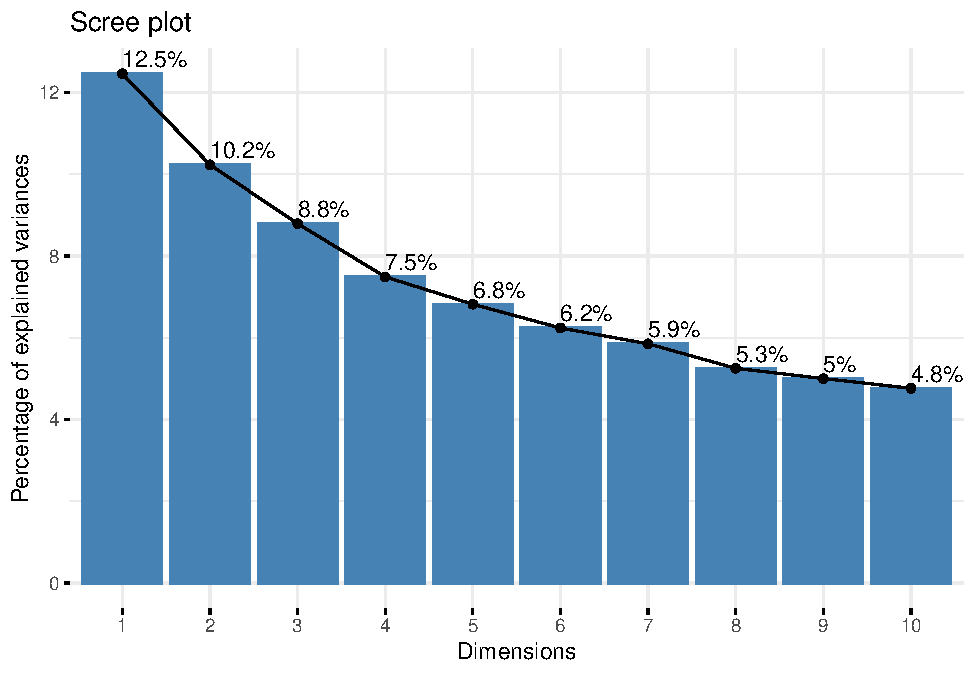
\includegraphics{Average-User-MCA_files/figure-latex/mca enjoyed all-1.pdf}

\begin{Shaded}
\begin{Highlighting}[]
\KeywordTok{fviz_mca_var}\NormalTok{(search.MCA, }\DataTypeTok{choice =} \StringTok{"mca.cor"}\NormalTok{, }\DataTypeTok{repel =} \OtherTok{TRUE}\NormalTok{,}
             \DataTypeTok{ggtheme =} \KeywordTok{theme_minimal}\NormalTok{())}
\end{Highlighting}
\end{Shaded}

\begin{verbatim}
## Warning: ggrepel: 78 unlabeled data points (too many overlaps). Consider
## increasing max.overlaps
\end{verbatim}

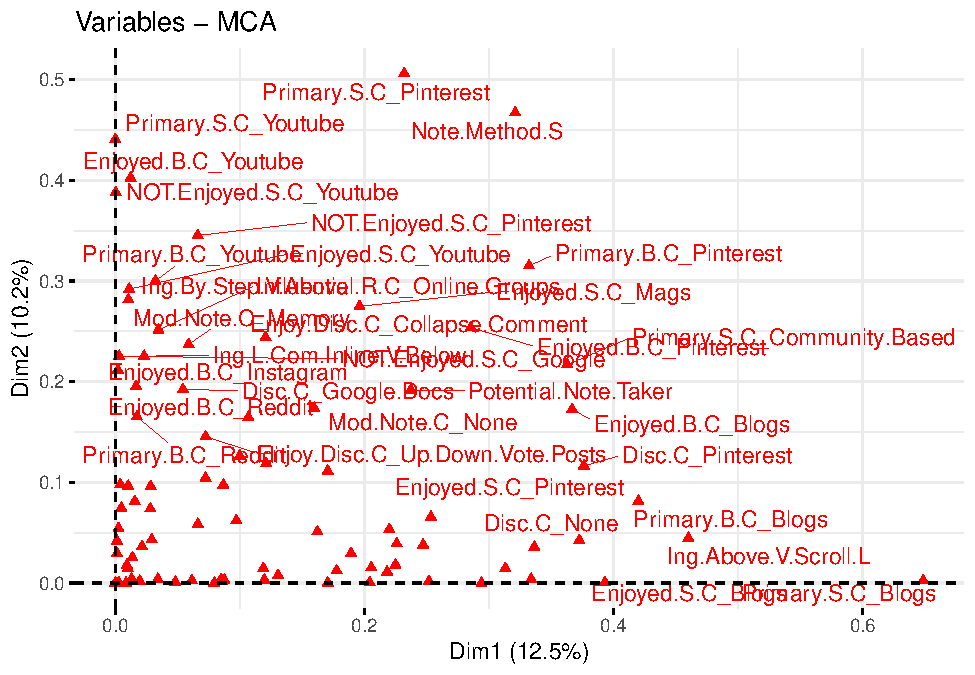
\includegraphics{Average-User-MCA_files/figure-latex/mca enjoyed all-2.pdf}

\begin{Shaded}
\begin{Highlighting}[]
\KeywordTok{fviz_mca_var}\NormalTok{(search.MCA, }\DataTypeTok{col.var =} \StringTok{"cos2"}\NormalTok{,}
             \DataTypeTok{gradient.cols =} \KeywordTok{c}\NormalTok{(}\StringTok{"#00AFBB"}\NormalTok{, }\StringTok{"#E7B800"}\NormalTok{, }\StringTok{"#FC4E07"}\NormalTok{),}
             \DataTypeTok{repel =} \OtherTok{TRUE}\NormalTok{, }\DataTypeTok{ggtheme =} \KeywordTok{theme_minimal}\NormalTok{())}
\end{Highlighting}
\end{Shaded}

\begin{verbatim}
## Warning: ggrepel: 195 unlabeled data points (too many overlaps). Consider
## increasing max.overlaps
\end{verbatim}

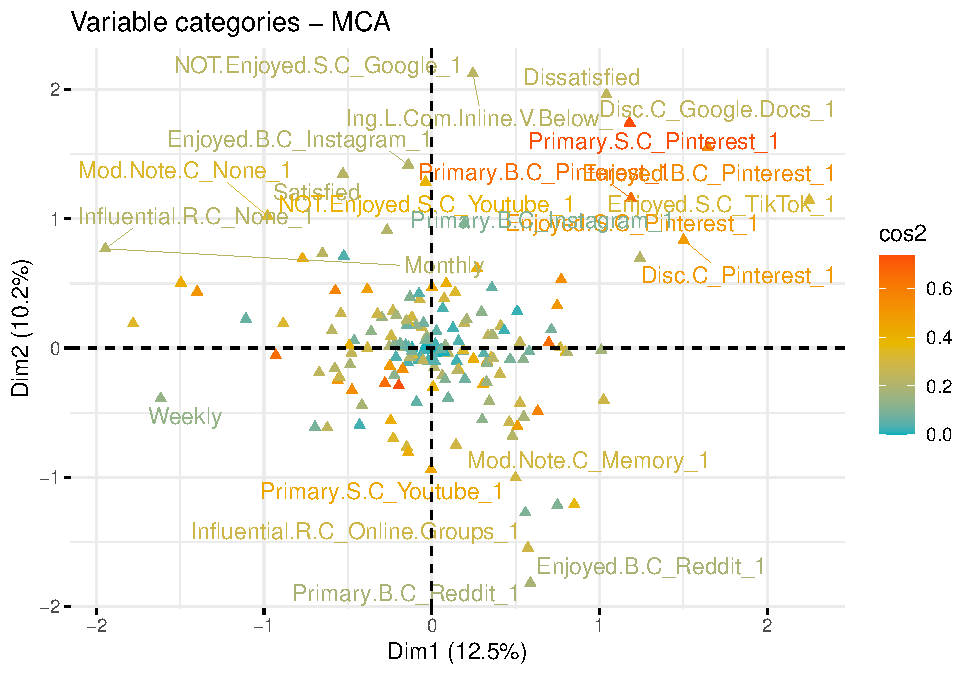
\includegraphics{Average-User-MCA_files/figure-latex/mca enjoyed all-3.pdf}

\hypertarget{what-do-users-not-enjoy}{%
\subsection{What Do Users NOT Enjoy?}\label{what-do-users-not-enjoy}}

\begin{Shaded}
\begin{Highlighting}[]
\NormalTok{NOT.enjoyed.data<-search.data[}\KeywordTok{c}\NormalTok{(}\StringTok{"Age"}\NormalTok{, }\StringTok{"Meal.Prepper"}\NormalTok{,}\StringTok{"Dietary.Restriction"}\NormalTok{,}\StringTok{"Home.Cook.Rate"}\NormalTok{,}\StringTok{"Primary.Format.C"}\NormalTok{,}\StringTok{"Primary.S.C"}\NormalTok{,}
            \StringTok{"NOT.Enjoyed.S.C"}\NormalTok{,}\StringTok{"Primary.B.C"}\NormalTok{,}\StringTok{"NOT.Enjoyed.B.C"}\NormalTok{,}\StringTok{"Ing.L.V.Above"}\NormalTok{,}
            \StringTok{"Ing.L.Com.Inline.V.Below"}\NormalTok{,}\StringTok{"Ing.Above.Com.Below.V.Inline"}\NormalTok{,  }\StringTok{"Ing.By.Step.V.Above"}\NormalTok{,  }\StringTok{"Ing.By.Step.V.Scroll.L"}\NormalTok{,}
            \StringTok{"Ing.Above.V.Scroll.L"}\NormalTok{)]}

\NormalTok{NOT.enjoyed.data.clean<-}\KeywordTok{cleaner.S}\NormalTok{(NOT.enjoyed.data)}
\NormalTok{search.MCA=}\KeywordTok{MCA}\NormalTok{(NOT.enjoyed.data.clean,}\DataTypeTok{graph=}\OtherTok{FALSE}\NormalTok{)}
\KeywordTok{fviz_screeplot}\NormalTok{(search.MCA,}\DataTypeTok{addlabels=}\NormalTok{T)}
\end{Highlighting}
\end{Shaded}

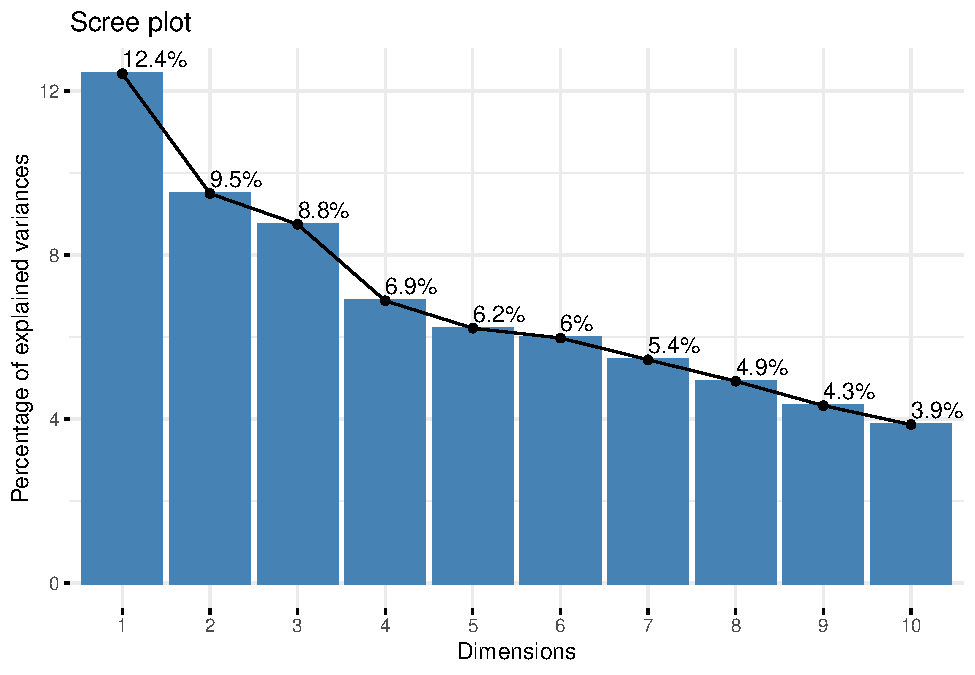
\includegraphics{Average-User-MCA_files/figure-latex/mca not enjoyed all-1.pdf}

\begin{Shaded}
\begin{Highlighting}[]
\KeywordTok{fviz_mca_var}\NormalTok{(search.MCA, }\DataTypeTok{choice =} \StringTok{"mca.cor"}\NormalTok{, }\DataTypeTok{repel =} \OtherTok{TRUE}\NormalTok{,}
             \DataTypeTok{ggtheme =} \KeywordTok{theme_minimal}\NormalTok{())}
\end{Highlighting}
\end{Shaded}

\begin{verbatim}
## Warning: ggrepel: 26 unlabeled data points (too many overlaps). Consider
## increasing max.overlaps
\end{verbatim}

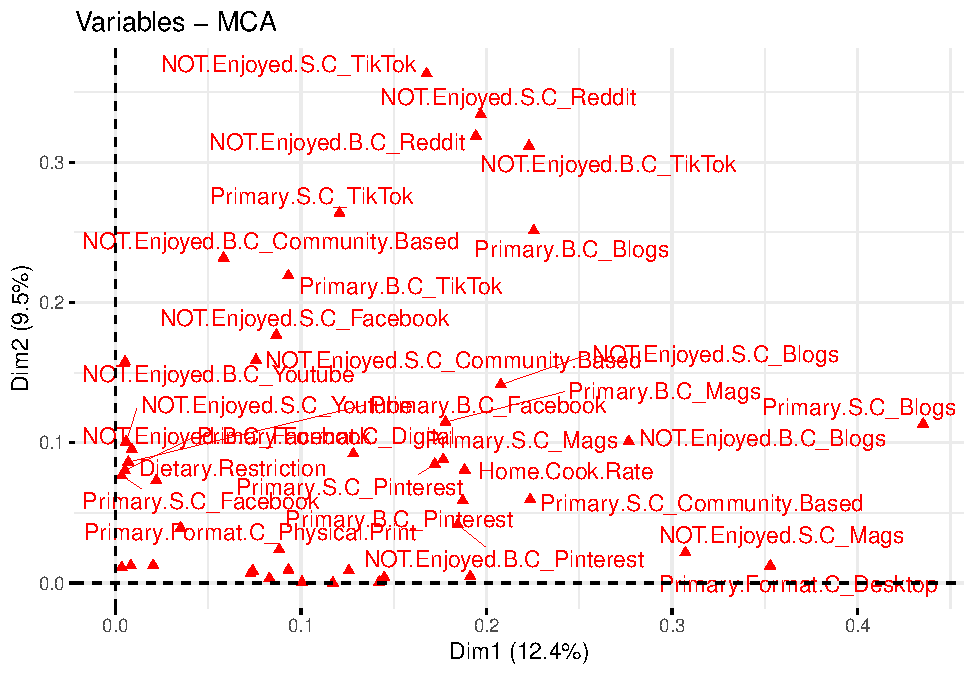
\includegraphics{Average-User-MCA_files/figure-latex/mca not enjoyed all-2.pdf}

\begin{Shaded}
\begin{Highlighting}[]
\KeywordTok{fviz_mca_var}\NormalTok{(search.MCA, }\DataTypeTok{col.var =} \StringTok{"cos2"}\NormalTok{,}
             \DataTypeTok{gradient.cols =} \KeywordTok{c}\NormalTok{(}\StringTok{"#00AFBB"}\NormalTok{, }\StringTok{"#E7B800"}\NormalTok{, }\StringTok{"#FC4E07"}\NormalTok{),}
             \DataTypeTok{repel =} \OtherTok{TRUE}\NormalTok{, }\DataTypeTok{ggtheme =} \KeywordTok{theme_minimal}\NormalTok{())}
\end{Highlighting}
\end{Shaded}

\begin{verbatim}
## Warning: ggrepel: 101 unlabeled data points (too many overlaps). Consider
## increasing max.overlaps
\end{verbatim}

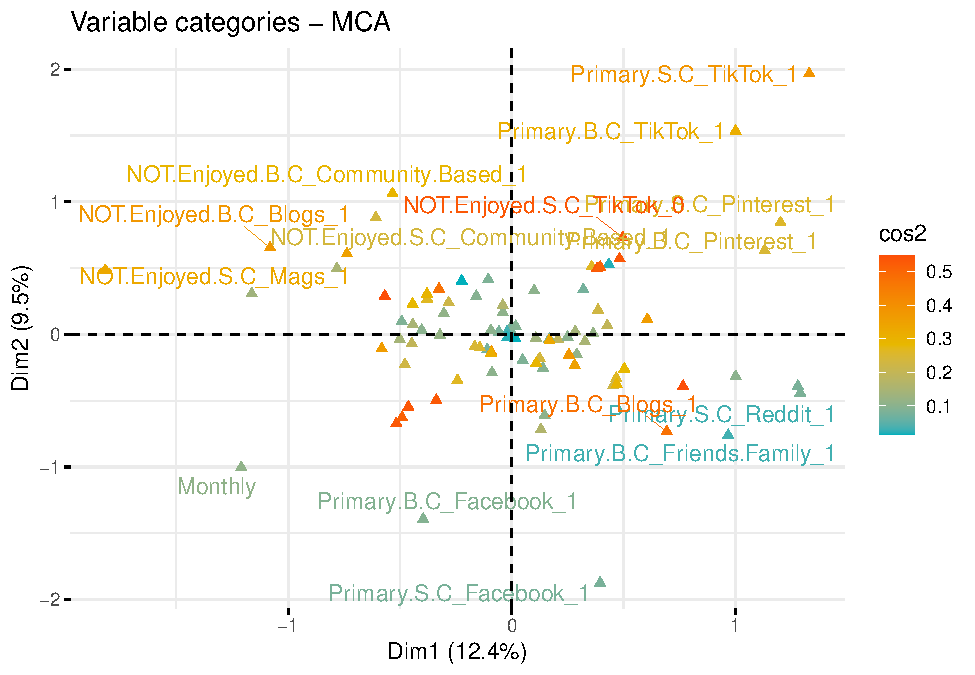
\includegraphics{Average-User-MCA_files/figure-latex/mca not enjoyed all-3.pdf}

\hypertarget{searching}{%
\subsection{Searching?}\label{searching}}

\begin{Shaded}
\begin{Highlighting}[]
\NormalTok{searching.data<-search.data[}\KeywordTok{c}\NormalTok{(}\StringTok{"Age"}\NormalTok{, }\StringTok{"Meal.Prepper"}\NormalTok{,}\StringTok{"Dietary.Restriction"}\NormalTok{,}\StringTok{"Home.Cook.Rate"}\NormalTok{,}\StringTok{"Primary.Format.C"}\NormalTok{,}\StringTok{"Primary.S.C"}\NormalTok{,}
            \StringTok{"Enjoyed.S.C"}\NormalTok{,}\StringTok{"NOT.Enjoyed.S.C"}\NormalTok{,}\StringTok{"Recipe.Search.F"}\NormalTok{,}\StringTok{"Repeat.S.F"}\NormalTok{,}\StringTok{"Browse.Search.F"}\NormalTok{,}\StringTok{"Click.Rate"}\NormalTok{,}
            \StringTok{"Search.Browse.Same"}\NormalTok{, }\StringTok{"Influential.R.C"}\NormalTok{,}\StringTok{"Seek.R.F"}\NormalTok{, }\StringTok{"Save.F"}\NormalTok{,}\StringTok{"Save.C"}\NormalTok{,}\StringTok{"Ing.L.V.Above"}\NormalTok{,}
            \StringTok{"Ing.L.Com.Inline.V.Below"}\NormalTok{,}\StringTok{"Ing.Above.Com.Below.V.Inline"}\NormalTok{,  }\StringTok{"Ing.By.Step.V.Above"}\NormalTok{,  }\StringTok{"Ing.By.Step.V.Scroll.L"}\NormalTok{,}
            \StringTok{"Ing.Above.V.Scroll.L"}\NormalTok{)]}

\NormalTok{searching.data.clean<-}\KeywordTok{cleaner.S}\NormalTok{(searching.data)}
\NormalTok{search.MCA=}\KeywordTok{MCA}\NormalTok{(searching.data.clean,}\DataTypeTok{graph=}\OtherTok{FALSE}\NormalTok{)}
\KeywordTok{fviz_screeplot}\NormalTok{(search.MCA,}\DataTypeTok{addlabels=}\NormalTok{T)}
\end{Highlighting}
\end{Shaded}

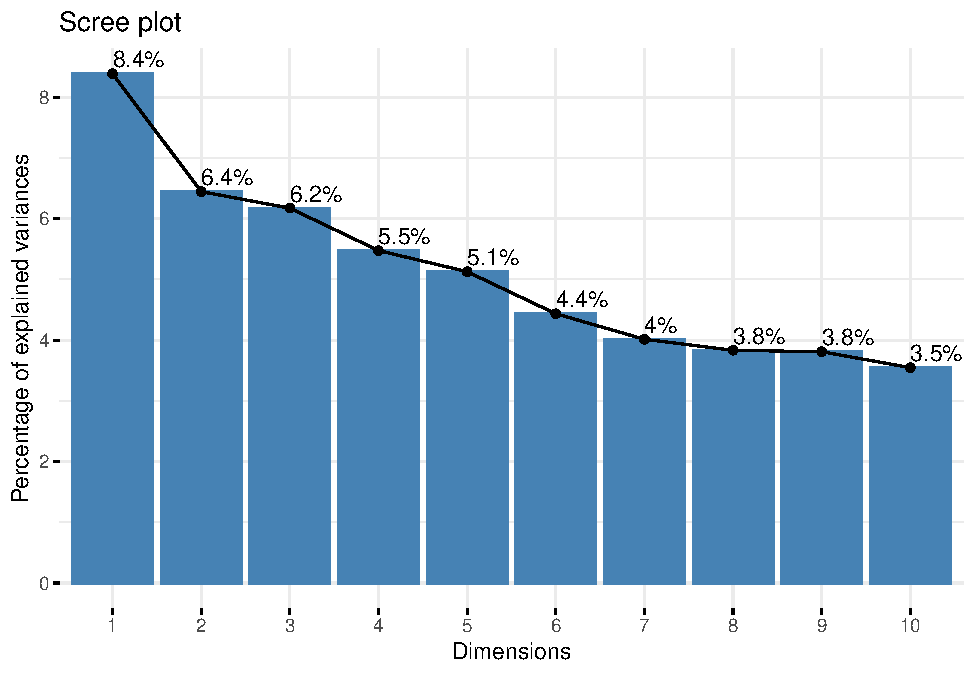
\includegraphics{Average-User-MCA_files/figure-latex/mca searching all-1.pdf}

\begin{Shaded}
\begin{Highlighting}[]
\KeywordTok{fviz_mca_var}\NormalTok{(search.MCA, }\DataTypeTok{choice =} \StringTok{"mca.cor"}\NormalTok{, }\DataTypeTok{repel =} \OtherTok{TRUE}\NormalTok{,}
             \DataTypeTok{ggtheme =} \KeywordTok{theme_minimal}\NormalTok{())}
\end{Highlighting}
\end{Shaded}

\begin{verbatim}
## Warning: ggrepel: 44 unlabeled data points (too many overlaps). Consider
## increasing max.overlaps
\end{verbatim}

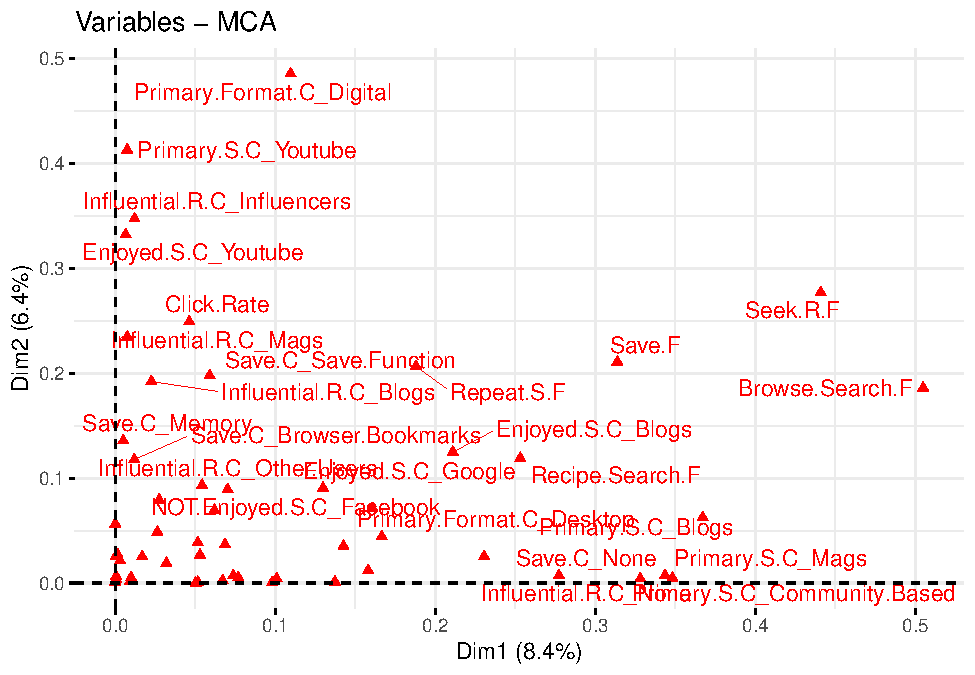
\includegraphics{Average-User-MCA_files/figure-latex/mca searching all-2.pdf}

\begin{Shaded}
\begin{Highlighting}[]
\KeywordTok{fviz_mca_var}\NormalTok{(search.MCA, }\DataTypeTok{col.var =} \StringTok{"cos2"}\NormalTok{,}
             \DataTypeTok{gradient.cols =} \KeywordTok{c}\NormalTok{(}\StringTok{"#00AFBB"}\NormalTok{, }\StringTok{"#E7B800"}\NormalTok{, }\StringTok{"#FC4E07"}\NormalTok{),}
             \DataTypeTok{repel =} \OtherTok{TRUE}\NormalTok{, }\DataTypeTok{ggtheme =} \KeywordTok{theme_minimal}\NormalTok{())}
\end{Highlighting}
\end{Shaded}

\begin{verbatim}
## Warning: ggrepel: 151 unlabeled data points (too many overlaps). Consider
## increasing max.overlaps
\end{verbatim}

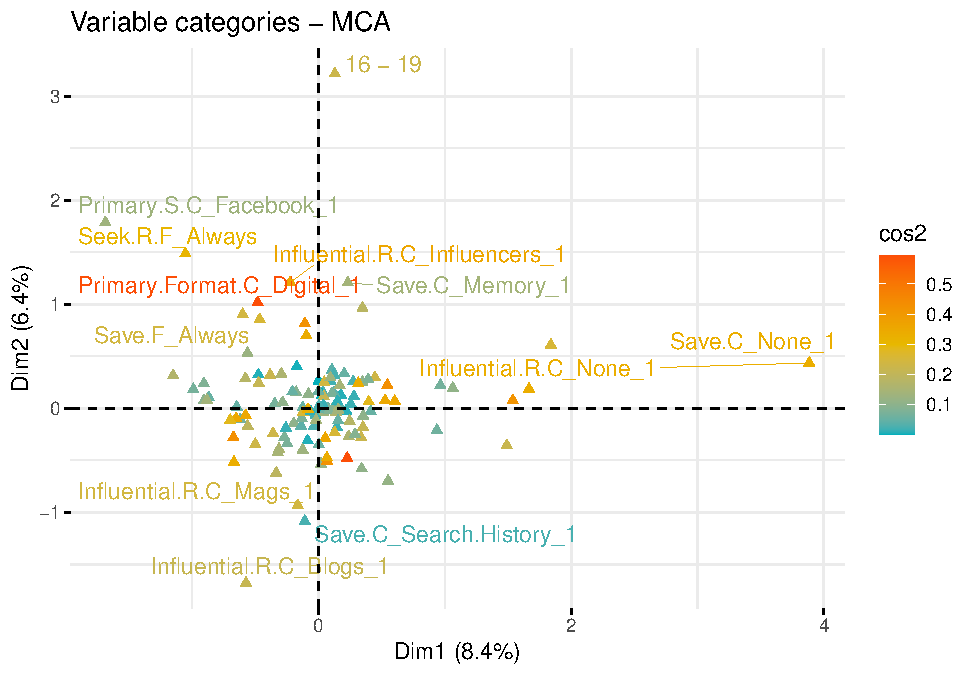
\includegraphics{Average-User-MCA_files/figure-latex/mca searching all-3.pdf}

\hypertarget{browsing}{%
\subsection{Browsing?}\label{browsing}}

\begin{Shaded}
\begin{Highlighting}[]
\NormalTok{searching.data<-search.data[}\KeywordTok{c}\NormalTok{(}\StringTok{"Age"}\NormalTok{, }\StringTok{"Meal.Prepper"}\NormalTok{,}\StringTok{"Dietary.Restriction"}\NormalTok{,}\StringTok{"Home.Cook.Rate"}\NormalTok{,}\StringTok{"Primary.Format.C"}\NormalTok{,}\StringTok{"Browse.Search.F"}\NormalTok{,}
            \StringTok{"Search.Browse.Same"}\NormalTok{,}\StringTok{"Primary.B.C"}\NormalTok{,}\StringTok{"Enjoyed.B.C"}\NormalTok{,}\StringTok{"NOT.Enjoyed.B.C"}\NormalTok{,}\StringTok{"Ing.L.V.Above"}\NormalTok{,}
            \StringTok{"Ing.L.Com.Inline.V.Below"}\NormalTok{,}\StringTok{"Ing.Above.Com.Below.V.Inline"}\NormalTok{,  }\StringTok{"Ing.By.Step.V.Above"}\NormalTok{,  }\StringTok{"Ing.By.Step.V.Scroll.L"}\NormalTok{,}
            \StringTok{"Ing.Above.V.Scroll.L"}\NormalTok{)]}

\NormalTok{searching.data.clean<-}\KeywordTok{cleaner.S}\NormalTok{(searching.data)}
\NormalTok{search.MCA=}\KeywordTok{MCA}\NormalTok{(searching.data.clean,}\DataTypeTok{graph=}\OtherTok{FALSE}\NormalTok{)}
\KeywordTok{fviz_screeplot}\NormalTok{(search.MCA,}\DataTypeTok{addlabels=}\NormalTok{T)}
\end{Highlighting}
\end{Shaded}

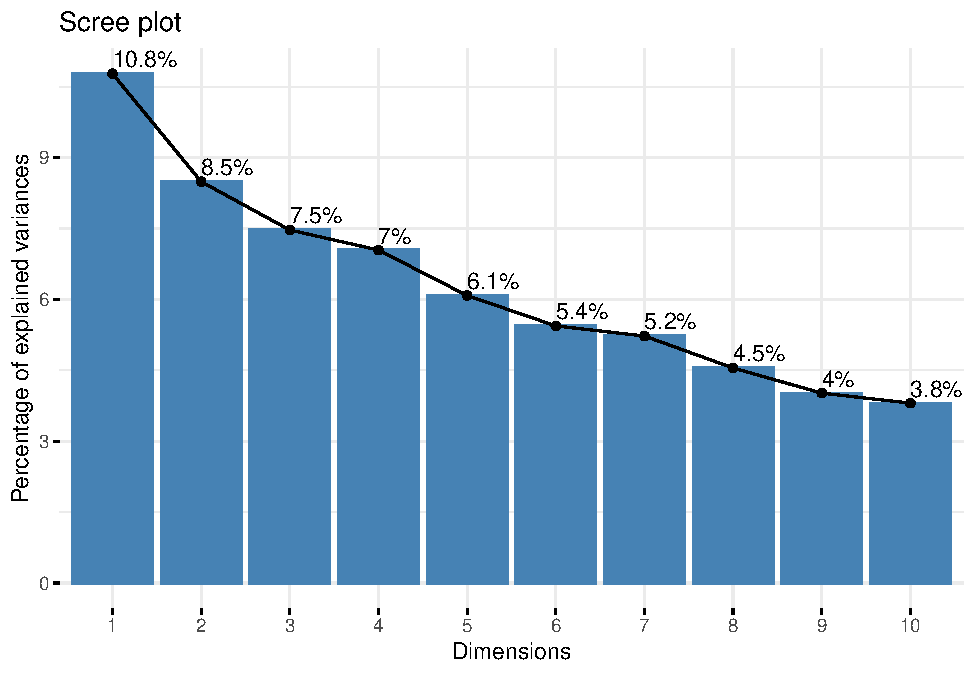
\includegraphics{Average-User-MCA_files/figure-latex/mca browsing all-1.pdf}

\begin{Shaded}
\begin{Highlighting}[]
\KeywordTok{fviz_mca_var}\NormalTok{(search.MCA, }\DataTypeTok{choice =} \StringTok{"mca.cor"}\NormalTok{, }\DataTypeTok{repel =} \OtherTok{TRUE}\NormalTok{,}
             \DataTypeTok{ggtheme =} \KeywordTok{theme_minimal}\NormalTok{())}
\end{Highlighting}
\end{Shaded}

\begin{verbatim}
## Warning: ggrepel: 27 unlabeled data points (too many overlaps). Consider
## increasing max.overlaps
\end{verbatim}

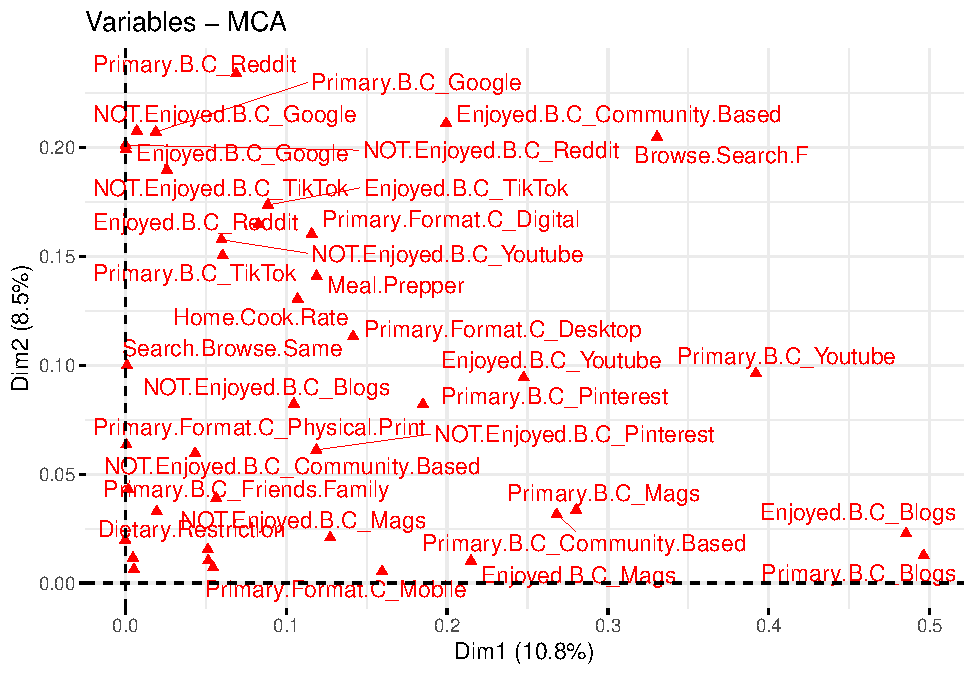
\includegraphics{Average-User-MCA_files/figure-latex/mca browsing all-2.pdf}

\begin{Shaded}
\begin{Highlighting}[]
\KeywordTok{fviz_mca_var}\NormalTok{(search.MCA, }\DataTypeTok{col.var =} \StringTok{"cos2"}\NormalTok{,}
             \DataTypeTok{gradient.cols =} \KeywordTok{c}\NormalTok{(}\StringTok{"#00AFBB"}\NormalTok{, }\StringTok{"#E7B800"}\NormalTok{, }\StringTok{"#FC4E07"}\NormalTok{),}
             \DataTypeTok{repel =} \OtherTok{TRUE}\NormalTok{, }\DataTypeTok{ggtheme =} \KeywordTok{theme_minimal}\NormalTok{())}
\end{Highlighting}
\end{Shaded}

\begin{verbatim}
## Warning: ggrepel: 88 unlabeled data points (too many overlaps). Consider
## increasing max.overlaps
\end{verbatim}

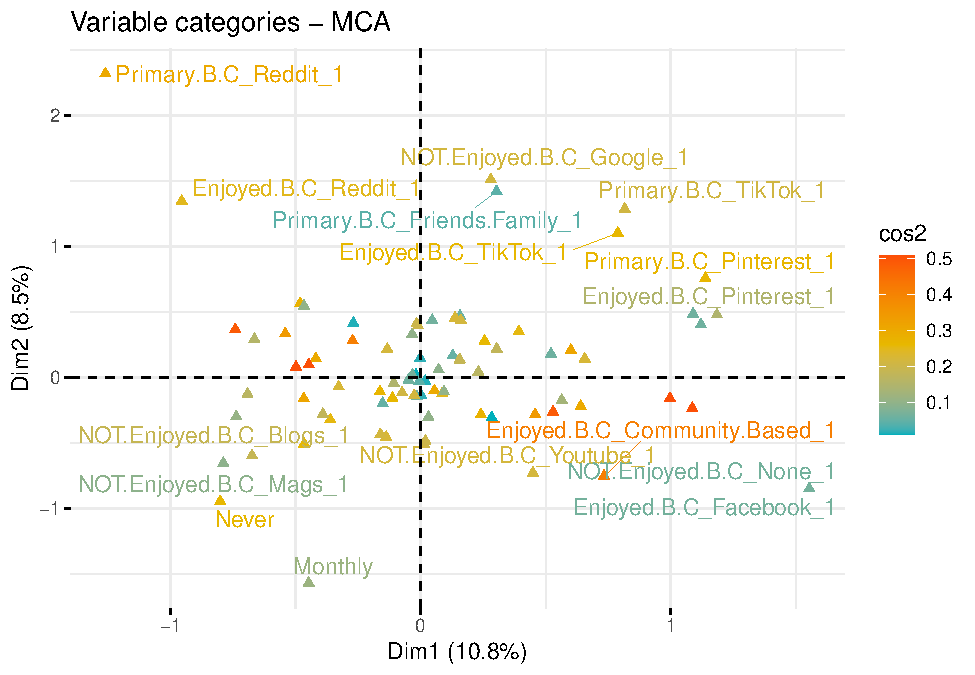
\includegraphics{Average-User-MCA_files/figure-latex/mca browsing all-3.pdf}

\hypertarget{review-discuss}{%
\subsection{Review \& Discuss?}\label{review-discuss}}

\begin{Shaded}
\begin{Highlighting}[]
\NormalTok{discussion.data<-search.data[}\KeywordTok{c}\NormalTok{(}\StringTok{"Age"}\NormalTok{, }\StringTok{"Meal.Prepper"}\NormalTok{,}\StringTok{"Dietary.Restriction"}\NormalTok{,}\StringTok{"Home.Cook.Rate"}\NormalTok{,}\StringTok{"Primary.Format.C"}\NormalTok{,}\StringTok{"Primary.R.C"}\NormalTok{, }\StringTok{"Influential.R.C"}\NormalTok{, }
            \StringTok{"Use.R.F"}\NormalTok{,}\StringTok{"Seek.R.F"}\NormalTok{, }\StringTok{"R.F"}\NormalTok{,}\StringTok{"Disc.F"}\NormalTok{,}\StringTok{"Read.Disc.F"}\NormalTok{,}\StringTok{"Disc.C"}\NormalTok{,}\StringTok{"Enjoy.Disc.C"}\NormalTok{,}\StringTok{"Ing.L.V.Above"}\NormalTok{,}
            \StringTok{"Ing.L.Com.Inline.V.Below"}\NormalTok{,}\StringTok{"Ing.Above.Com.Below.V.Inline"}\NormalTok{,  }\StringTok{"Ing.By.Step.V.Above"}\NormalTok{,  }\StringTok{"Ing.By.Step.V.Scroll.L"}\NormalTok{,}
            \StringTok{"Ing.Above.V.Scroll.L"}\NormalTok{)]}
\NormalTok{discussion.data.clean<-}\KeywordTok{cleaner.S}\NormalTok{(discussion.data)}
\NormalTok{search.MCA=}\KeywordTok{MCA}\NormalTok{(discussion.data.clean,}\DataTypeTok{graph=}\OtherTok{FALSE}\NormalTok{)}
\KeywordTok{fviz_screeplot}\NormalTok{(search.MCA,}\DataTypeTok{addlabels=}\NormalTok{T)}
\end{Highlighting}
\end{Shaded}

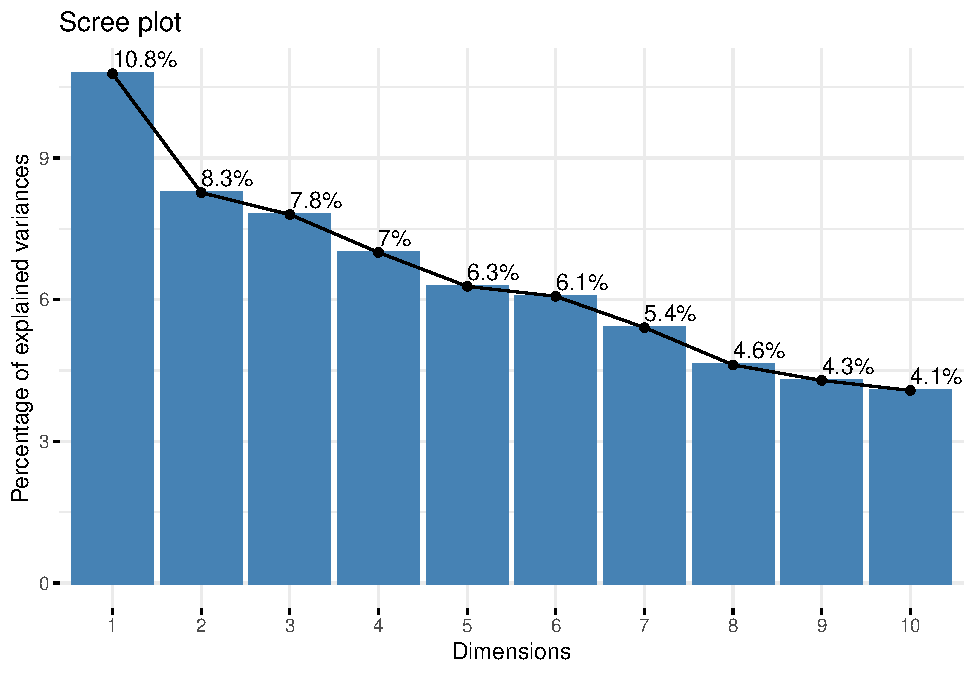
\includegraphics{Average-User-MCA_files/figure-latex/mca social all-1.pdf}

\begin{Shaded}
\begin{Highlighting}[]
\KeywordTok{fviz_mca_var}\NormalTok{(search.MCA, }\DataTypeTok{choice =} \StringTok{"mca.cor"}\NormalTok{, }\DataTypeTok{repel =} \OtherTok{TRUE}\NormalTok{,}
             \DataTypeTok{ggtheme =} \KeywordTok{theme_minimal}\NormalTok{())}
\end{Highlighting}
\end{Shaded}

\begin{verbatim}
## Warning: ggrepel: 35 unlabeled data points (too many overlaps). Consider
## increasing max.overlaps
\end{verbatim}

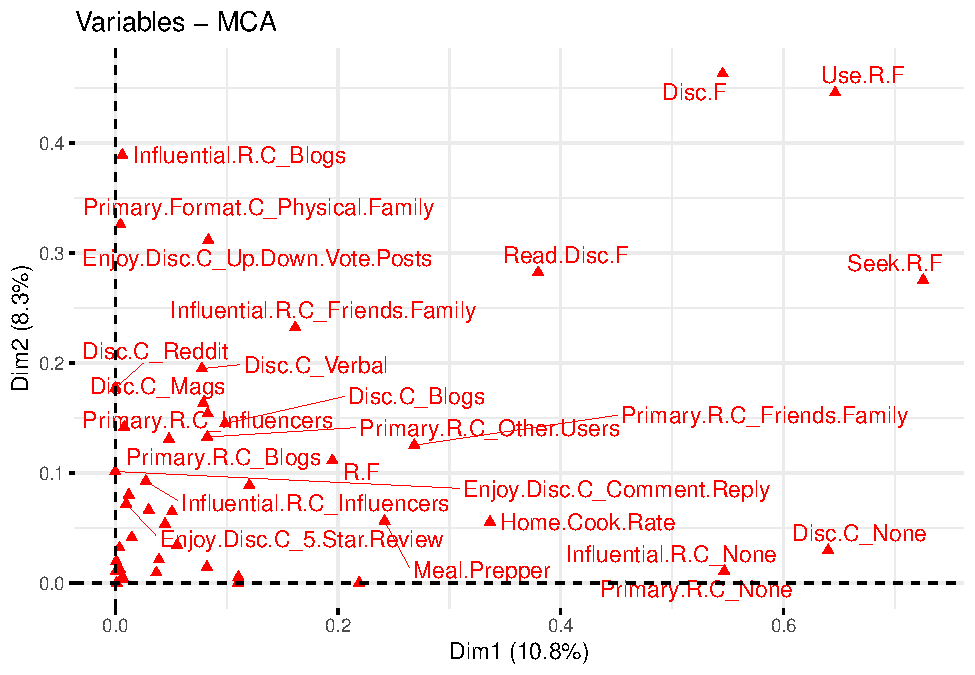
\includegraphics{Average-User-MCA_files/figure-latex/mca social all-2.pdf}

\begin{Shaded}
\begin{Highlighting}[]
\KeywordTok{fviz_mca_var}\NormalTok{(search.MCA, }\DataTypeTok{col.var =} \StringTok{"cos2"}\NormalTok{,}
             \DataTypeTok{gradient.cols =} \KeywordTok{c}\NormalTok{(}\StringTok{"#00AFBB"}\NormalTok{, }\StringTok{"#E7B800"}\NormalTok{, }\StringTok{"#FC4E07"}\NormalTok{),}
             \DataTypeTok{repel =} \OtherTok{TRUE}\NormalTok{, }\DataTypeTok{ggtheme =} \KeywordTok{theme_minimal}\NormalTok{())}
\end{Highlighting}
\end{Shaded}

\begin{verbatim}
## Warning: ggrepel: 121 unlabeled data points (too many overlaps). Consider
## increasing max.overlaps
\end{verbatim}

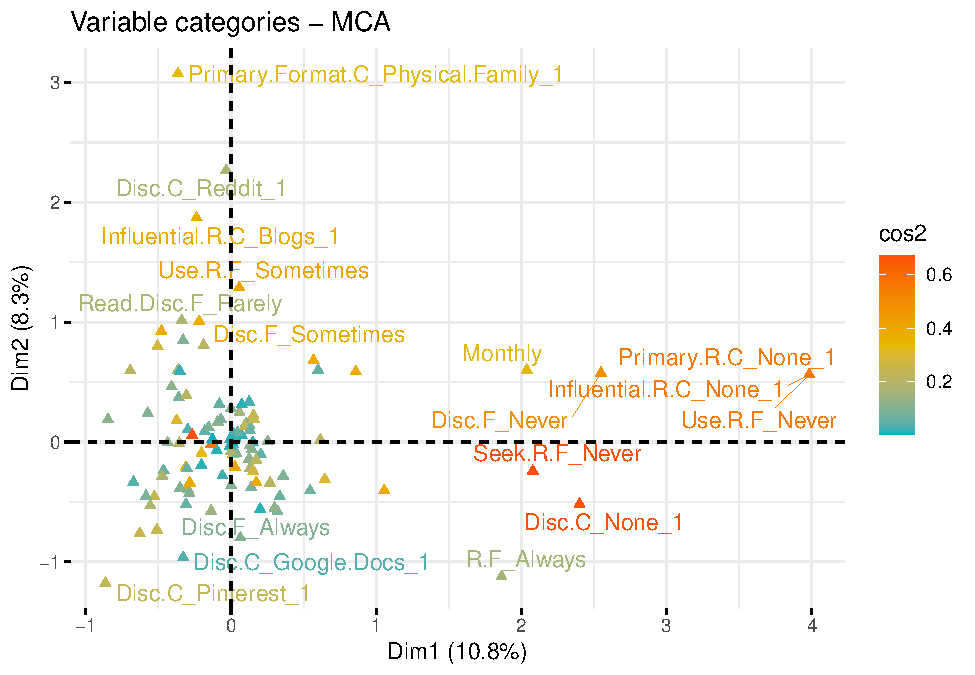
\includegraphics{Average-User-MCA_files/figure-latex/mca social all-3.pdf}

\hypertarget{frequency}{%
\subsubsection{Frequency}\label{frequency}}

\begin{Shaded}
\begin{Highlighting}[]
\NormalTok{freq<-}\StringTok{ }\NormalTok{search.data[}\KeywordTok{c}\NormalTok{(}\StringTok{"Meal.Prepper"}\NormalTok{, }\StringTok{"Age"}\NormalTok{,}\StringTok{"Home.Cook.Rate"}\NormalTok{,}\StringTok{"Recipe.Search.F"}\NormalTok{,}\StringTok{"Repeat.S.F"}\NormalTok{,}\StringTok{"Browse.Search.F"}\NormalTok{,}\StringTok{"Click.Rate"}\NormalTok{,}
            \StringTok{"Use.R.F"}\NormalTok{,}\StringTok{"Seek.R.F"}\NormalTok{, }\StringTok{"R.F"}\NormalTok{,}\StringTok{"Save.F"}\NormalTok{,}\StringTok{"Mod.F"}\NormalTok{, }\StringTok{"Mod.Note.F"}\NormalTok{,}\StringTok{"Disc.F"}\NormalTok{,}\StringTok{"Read.Disc.F"}\NormalTok{,}\StringTok{"Ing.L.V.Above"}\NormalTok{,}
            \StringTok{"Ing.L.Com.Inline.V.Below"}\NormalTok{,}\StringTok{"Ing.Above.Com.Below.V.Inline"}\NormalTok{,  }\StringTok{"Ing.By.Step.V.Above"}\NormalTok{,  }\StringTok{"Ing.By.Step.V.Scroll.L"}\NormalTok{,}
            \StringTok{"Ing.Above.V.Scroll.L"}\NormalTok{)]}
\NormalTok{cols<-}\KeywordTok{names}\NormalTok{(freq)}
\NormalTok{freq<-}\KeywordTok{lapply}\NormalTok{(freq[cols], as.factor)}
\NormalTok{freq<-}\KeywordTok{data.frame}\NormalTok{(freq)}
\NormalTok{search.MCA=}\KeywordTok{MCA}\NormalTok{(freq,}\DataTypeTok{graph=}\OtherTok{FALSE}\NormalTok{)}
\KeywordTok{fviz_screeplot}\NormalTok{(search.MCA,}\DataTypeTok{addlabels=}\NormalTok{T)}
\end{Highlighting}
\end{Shaded}

\includegraphics{Average-User-MCA_files/figure-latex/freq-1.pdf}

\begin{Shaded}
\begin{Highlighting}[]
\KeywordTok{fviz_mca_var}\NormalTok{(search.MCA, }\DataTypeTok{choice =} \StringTok{"mca.cor"}\NormalTok{, }\DataTypeTok{repel =} \OtherTok{TRUE}\NormalTok{,}
             \DataTypeTok{ggtheme =} \KeywordTok{theme_minimal}\NormalTok{())}
\end{Highlighting}
\end{Shaded}

\includegraphics{Average-User-MCA_files/figure-latex/freq-2.pdf}

\begin{Shaded}
\begin{Highlighting}[]
\KeywordTok{fviz_mca_var}\NormalTok{(search.MCA, }\DataTypeTok{col.var =} \StringTok{"cos2"}\NormalTok{,}
             \DataTypeTok{gradient.cols =} \KeywordTok{c}\NormalTok{(}\StringTok{"#00AFBB"}\NormalTok{, }\StringTok{"#E7B800"}\NormalTok{, }\StringTok{"#FC4E07"}\NormalTok{),}
             \DataTypeTok{repel =} \OtherTok{TRUE}\NormalTok{, }\DataTypeTok{ggtheme =} \KeywordTok{theme_minimal}\NormalTok{())}
\end{Highlighting}
\end{Shaded}

\begin{verbatim}
## Warning: ggrepel: 79 unlabeled data points (too many overlaps). Consider
## increasing max.overlaps
\end{verbatim}

\includegraphics{Average-User-MCA_files/figure-latex/freq-3.pdf} \#
Stratify By Diet

\hypertarget{overview}{%
\subsection{Overview}\label{overview}}

Slightly More variance is captured in the components when we stratify by
diet.

\begin{Shaded}
\begin{Highlighting}[]
\NormalTok{cleaned.Diet.Yes<-}\KeywordTok{filter}\NormalTok{(search.data, Dietary.Restriction }\OperatorTok{==}\StringTok{ "Yes"}\NormalTok{)}
\NormalTok{cleaned.Diet.Yes<-cleaned.Diet.Yes}\OperatorTok\KeywordTok{select}\NormalTok{(}\OperatorTok{-}\KeywordTok{c}\NormalTok{(Dietary.Restriction))}
\CommentTok{# data.clean.Diet.Yes<-cleaner.S(cleaned.Diet.Yes)}
\CommentTok{# search.MCA=MCA(data.clean.Diet.Yes,graph=FALSE)}
\CommentTok{# fviz_screeplot(search.MCA,addlabels=T)}
\CommentTok{# fviz_mca_var(search.MCA, choice = "mca.cor", repel = TRUE,}
\CommentTok{#              ggtheme = theme_minimal())}
\CommentTok{# }
\CommentTok{# fviz_mca_var(search.MCA, col.var = "cos2",}
\CommentTok{#              gradient.cols = c("#00AFBB", "#E7B800", "#FC4E07"),}
\CommentTok{#              repel = TRUE, ggtheme = theme_minimal())}
\end{Highlighting}
\end{Shaded}

\begin{Shaded}
\begin{Highlighting}[]
\NormalTok{cleaned.Diet.No<-}\KeywordTok{filter}\NormalTok{(search.data, Dietary.Restriction }\OperatorTok{==}\StringTok{ "No"}\NormalTok{)}
\NormalTok{cleaned.Diet.No<-cleaned.Diet.No}\OperatorTok\KeywordTok{select}\NormalTok{(}\OperatorTok{-}\KeywordTok{c}\NormalTok{(Dietary.Restriction))}
\CommentTok{# data.clean.Diet.No<-cleaner.S(cleaned.Diet.No)}
\CommentTok{# search.MCA=MCA(data.clean.Diet.No,graph=FALSE)}
\CommentTok{# fviz_screeplot(search.MCA,addlabels=T)}
\CommentTok{# fviz_mca_var(search.MCA, choice = "mca.cor", repel = TRUE,}
\CommentTok{#              ggtheme = theme_minimal())}
\CommentTok{# }
\CommentTok{# fviz_mca_var(search.MCA, col.var = "cos2",}
\CommentTok{#              gradient.cols = c("#00AFBB", "#E7B800", "#FC4E07"),}
\CommentTok{#              repel = TRUE, ggtheme = theme_minimal())}
\end{Highlighting}
\end{Shaded}

\hypertarget{what-do-users-enjoy-1}{%
\subsubsection{What Do Users Enjoy?}\label{what-do-users-enjoy-1}}

\begin{Shaded}
\begin{Highlighting}[]
\NormalTok{enjoyed.data.diet<-cleaned.Diet.Yes[}\KeywordTok{c}\NormalTok{(}\StringTok{"Age"}\NormalTok{, }\StringTok{"Meal.Prepper"}\NormalTok{,}\StringTok{"Home.Cook.Rate"}\NormalTok{,}\StringTok{"Primary.Format.C"}\NormalTok{,}\StringTok{"Primary.S.C"}\NormalTok{,}
            \StringTok{"Enjoyed.S.C"}\NormalTok{,}\StringTok{"NOT.Enjoyed.S.C"}\NormalTok{,}\StringTok{"Primary.B.C"}\NormalTok{,}\StringTok{"Enjoyed.B.C"}\NormalTok{,}\StringTok{"Influential.R.C"}\NormalTok{, }
            \StringTok{"Mod.Note.C"}\NormalTok{, }
            \StringTok{"Note.Method.S"}\NormalTok{,}\StringTok{"Potential.Note.Taker"}\NormalTok{,}\StringTok{"Disc.C"}\NormalTok{,}\StringTok{"Enjoy.Disc.C"}\NormalTok{,}\StringTok{"Ing.L.V.Above"}\NormalTok{,}
            \StringTok{"Ing.L.Com.Inline.V.Below"}\NormalTok{,}\StringTok{"Ing.Above.Com.Below.V.Inline"}\NormalTok{,  }\StringTok{"Ing.By.Step.V.Above"}\NormalTok{,  }\StringTok{"Ing.By.Step.V.Scroll.L"}\NormalTok{,}
            \StringTok{"Ing.Above.V.Scroll.L"}\NormalTok{)]}

\NormalTok{enjoyed.data.clean<-}\KeywordTok{cleaner.S}\NormalTok{(enjoyed.data.diet)}
\NormalTok{search.MCA=}\KeywordTok{MCA}\NormalTok{(enjoyed.data.clean,}\DataTypeTok{graph=}\OtherTok{FALSE}\NormalTok{)}
\KeywordTok{fviz_screeplot}\NormalTok{(search.MCA,}\DataTypeTok{addlabels=}\NormalTok{T)}
\end{Highlighting}
\end{Shaded}

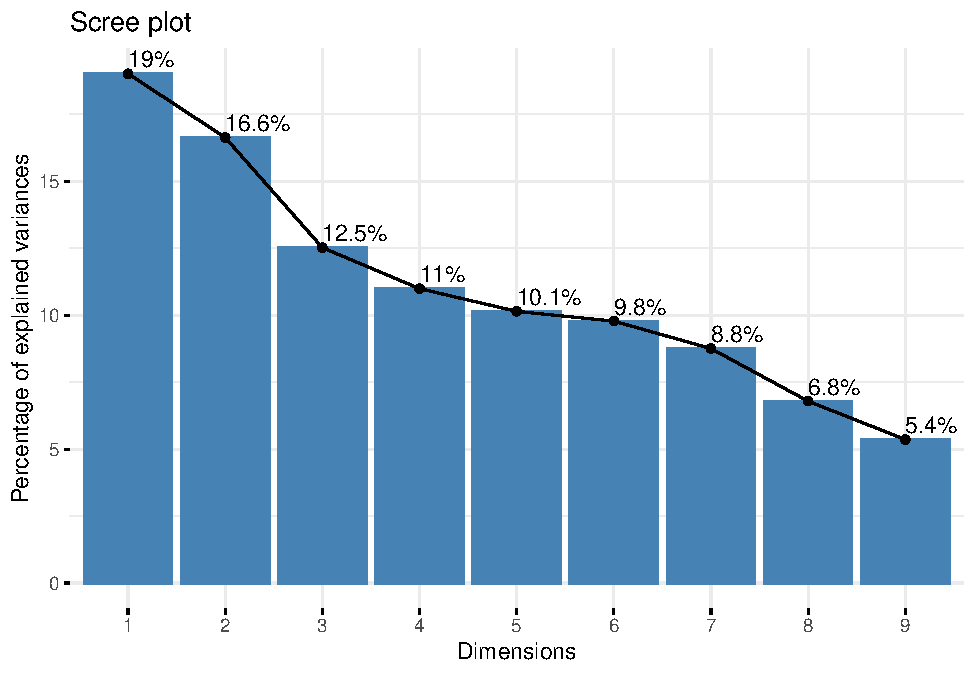
\includegraphics{Average-User-MCA_files/figure-latex/diet yes enjoy-1.pdf}

\begin{Shaded}
\begin{Highlighting}[]
\KeywordTok{fviz_mca_var}\NormalTok{(search.MCA, }\DataTypeTok{choice =} \StringTok{"mca.cor"}\NormalTok{, }\DataTypeTok{repel =} \OtherTok{TRUE}\NormalTok{,}
             \DataTypeTok{ggtheme =} \KeywordTok{theme_minimal}\NormalTok{())}
\end{Highlighting}
\end{Shaded}

\begin{verbatim}
## Warning: ggrepel: 65 unlabeled data points (too many overlaps). Consider
## increasing max.overlaps
\end{verbatim}

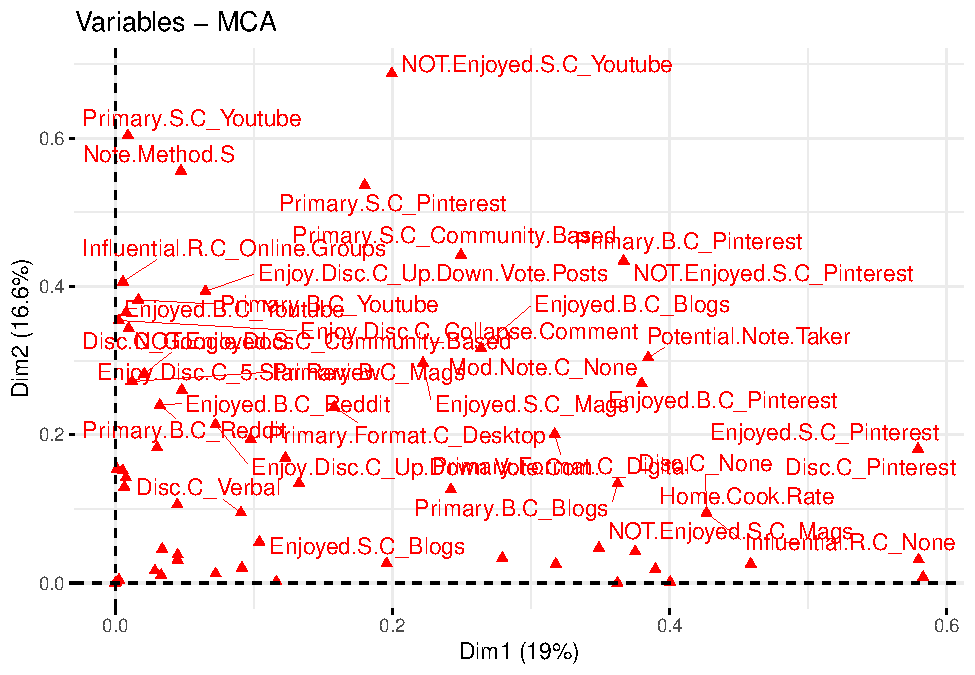
\includegraphics{Average-User-MCA_files/figure-latex/diet yes enjoy-2.pdf}

\begin{Shaded}
\begin{Highlighting}[]
\KeywordTok{fviz_mca_var}\NormalTok{(search.MCA, }\DataTypeTok{col.var =} \StringTok{"cos2"}\NormalTok{,}
             \DataTypeTok{gradient.cols =} \KeywordTok{c}\NormalTok{(}\StringTok{"#00AFBB"}\NormalTok{, }\StringTok{"#E7B800"}\NormalTok{, }\StringTok{"#FC4E07"}\NormalTok{),}
             \DataTypeTok{repel =} \OtherTok{TRUE}\NormalTok{, }\DataTypeTok{ggtheme =} \KeywordTok{theme_minimal}\NormalTok{())}
\end{Highlighting}
\end{Shaded}

\begin{verbatim}
## Warning: ggrepel: 183 unlabeled data points (too many overlaps). Consider
## increasing max.overlaps
\end{verbatim}

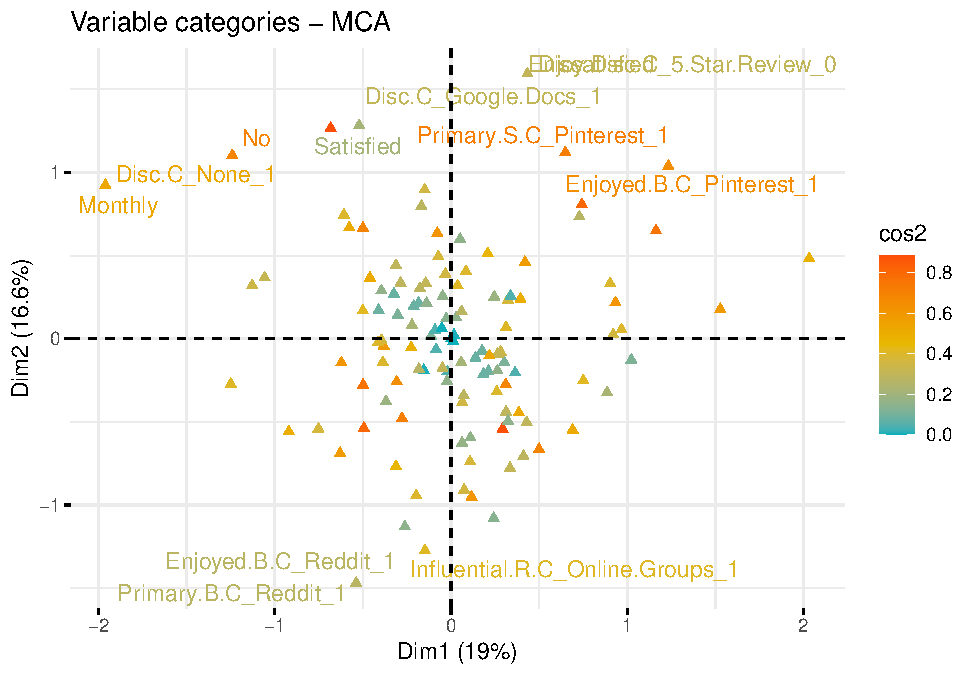
\includegraphics{Average-User-MCA_files/figure-latex/diet yes enjoy-3.pdf}

\begin{Shaded}
\begin{Highlighting}[]
\NormalTok{enjoyed.data.diet<-cleaned.Diet.No[}\KeywordTok{c}\NormalTok{(}\StringTok{"Age"}\NormalTok{,}\StringTok{"Meal.Prepper"}\NormalTok{,}\StringTok{"Home.Cook.Rate"}\NormalTok{,}
                                     \StringTok{"Primary.Format.C"}\NormalTok{,}\StringTok{"Primary.S.C"}\NormalTok{,}
                               \StringTok{"Enjoyed.S.C"}\NormalTok{,}\StringTok{"NOT.Enjoyed.S.C"}\NormalTok{,}\StringTok{"Primary.B.C"}\NormalTok{,}
                               \StringTok{"Enjoyed.B.C"}\NormalTok{,}\StringTok{"Influential.R.C"}\NormalTok{, }\StringTok{"Mod.Note.C"}\NormalTok{,}
                               \StringTok{"Note.Method.S"}\NormalTok{,}\StringTok{"Potential.Note.Taker"}\NormalTok{,}\StringTok{"Disc.C"}\NormalTok{,}\StringTok{"Enjoy.Disc.C"}\NormalTok{)]}

\NormalTok{enjoyed.data.clean<-}\KeywordTok{cleaner.S}\NormalTok{(enjoyed.data.diet)}
\NormalTok{search.MCA=}\KeywordTok{MCA}\NormalTok{(enjoyed.data.clean,}\DataTypeTok{graph=}\OtherTok{FALSE}\NormalTok{)}
\KeywordTok{fviz_screeplot}\NormalTok{(search.MCA,}\DataTypeTok{addlabels=}\NormalTok{T)}
\end{Highlighting}
\end{Shaded}

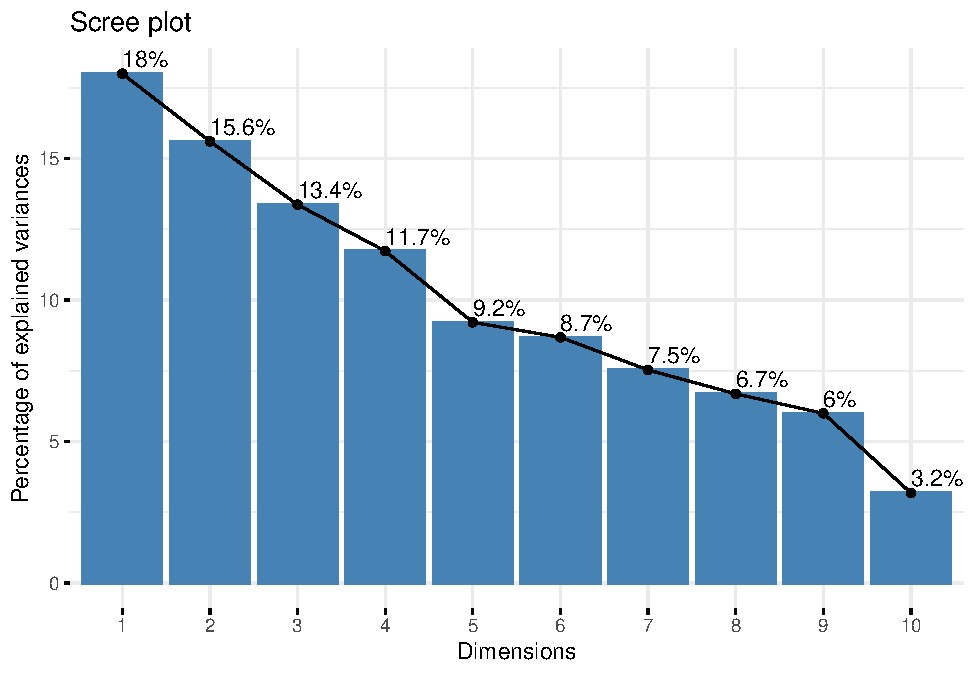
\includegraphics{Average-User-MCA_files/figure-latex/diet no enjoy-1.pdf}

\begin{Shaded}
\begin{Highlighting}[]
\KeywordTok{fviz_mca_var}\NormalTok{(search.MCA, }\DataTypeTok{choice =} \StringTok{"mca.cor"}\NormalTok{, }\DataTypeTok{repel =} \OtherTok{TRUE}\NormalTok{,}
             \DataTypeTok{ggtheme =} \KeywordTok{theme_minimal}\NormalTok{())}
\end{Highlighting}
\end{Shaded}

\begin{verbatim}
## Warning: ggrepel: 60 unlabeled data points (too many overlaps). Consider
## increasing max.overlaps
\end{verbatim}

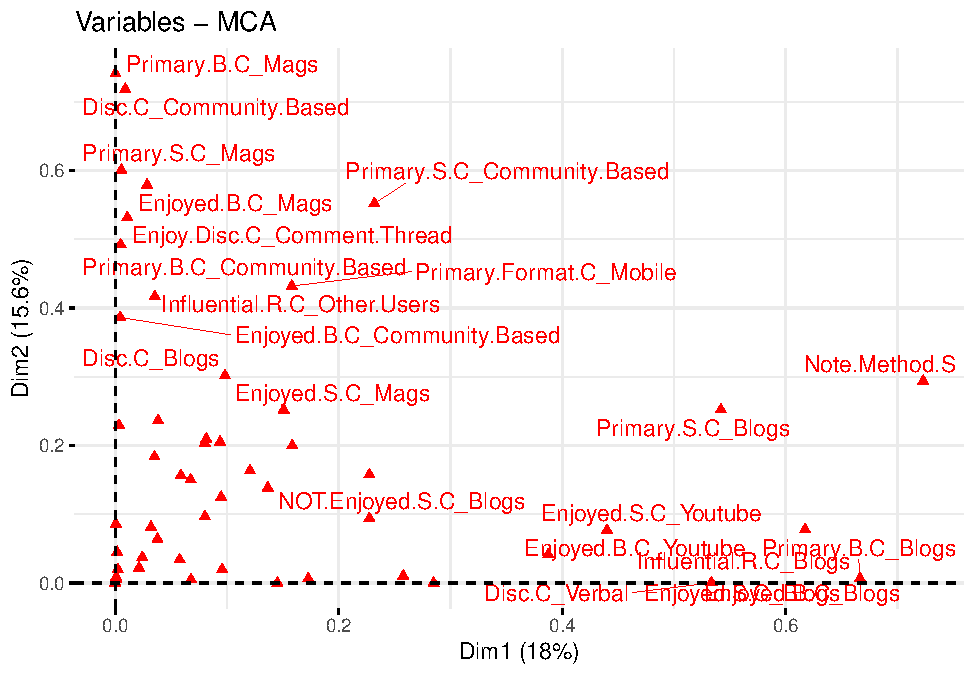
\includegraphics{Average-User-MCA_files/figure-latex/diet no enjoy-2.pdf}

\begin{Shaded}
\begin{Highlighting}[]
\KeywordTok{fviz_mca_var}\NormalTok{(search.MCA, }\DataTypeTok{col.var =} \StringTok{"cos2"}\NormalTok{,}
             \DataTypeTok{gradient.cols =} \KeywordTok{c}\NormalTok{(}\StringTok{"#00AFBB"}\NormalTok{, }\StringTok{"#E7B800"}\NormalTok{, }\StringTok{"#FC4E07"}\NormalTok{),}
             \DataTypeTok{repel =} \OtherTok{TRUE}\NormalTok{, }\DataTypeTok{ggtheme =} \KeywordTok{theme_minimal}\NormalTok{())}
\end{Highlighting}
\end{Shaded}

\begin{verbatim}
## Warning: ggrepel: 151 unlabeled data points (too many overlaps). Consider
## increasing max.overlaps
\end{verbatim}

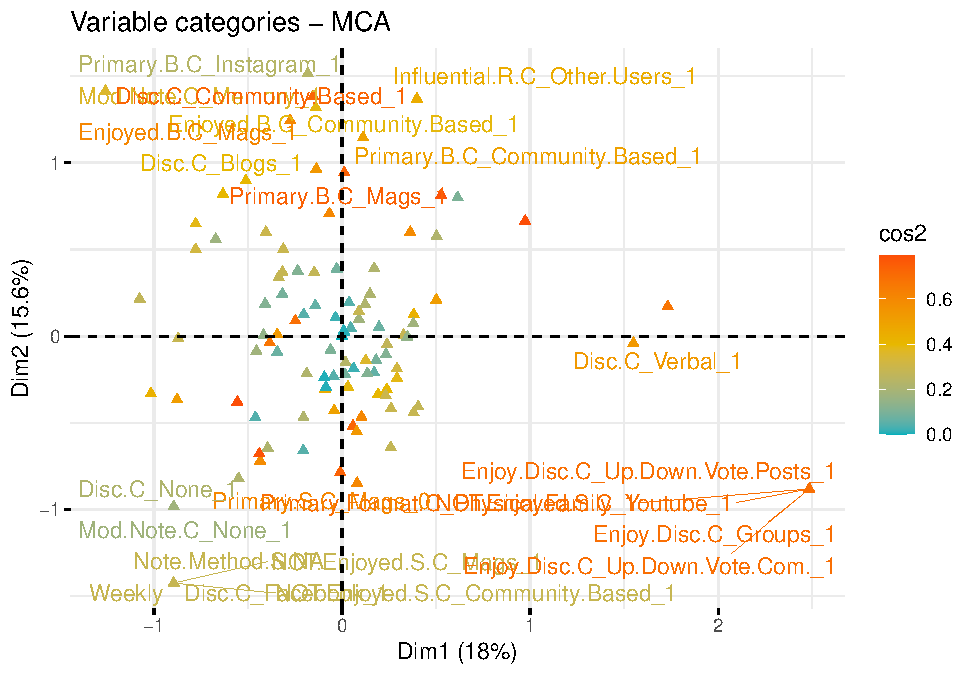
\includegraphics{Average-User-MCA_files/figure-latex/diet no enjoy-3.pdf}

\hypertarget{what-do-users-not-enjoy-1}{%
\subsubsection{What Do Users NOT
Enjoy?}\label{what-do-users-not-enjoy-1}}

\begin{Shaded}
\begin{Highlighting}[]
\NormalTok{NOT.enjoyed.data<-cleaned.Diet.Yes[}\KeywordTok{c}\NormalTok{(}\StringTok{"Age"}\NormalTok{, }\StringTok{"Meal.Prepper"}\NormalTok{,}\StringTok{"Home.Cook.Rate"}\NormalTok{,}\StringTok{"Primary.Format.C"}\NormalTok{,}\StringTok{"Primary.S.C"}\NormalTok{,}
            \StringTok{"NOT.Enjoyed.S.C"}\NormalTok{,}\StringTok{"Primary.B.C"}\NormalTok{,}\StringTok{"NOT.Enjoyed.B.C"}\NormalTok{,}\StringTok{"Ing.L.V.Above"}\NormalTok{,}
            \StringTok{"Ing.L.Com.Inline.V.Below"}\NormalTok{,}\StringTok{"Ing.Above.Com.Below.V.Inline"}\NormalTok{,  }\StringTok{"Ing.By.Step.V.Above"}\NormalTok{,  }\StringTok{"Ing.By.Step.V.Scroll.L"}\NormalTok{,}
            \StringTok{"Ing.Above.V.Scroll.L"}\NormalTok{)]}

\NormalTok{NOT.enjoyed.data.clean<-}\KeywordTok{cleaner.S}\NormalTok{(NOT.enjoyed.data)}
\NormalTok{search.MCA=}\KeywordTok{MCA}\NormalTok{(NOT.enjoyed.data.clean,}\DataTypeTok{graph=}\OtherTok{FALSE}\NormalTok{)}
\KeywordTok{fviz_screeplot}\NormalTok{(search.MCA,}\DataTypeTok{addlabels=}\NormalTok{T)}
\end{Highlighting}
\end{Shaded}

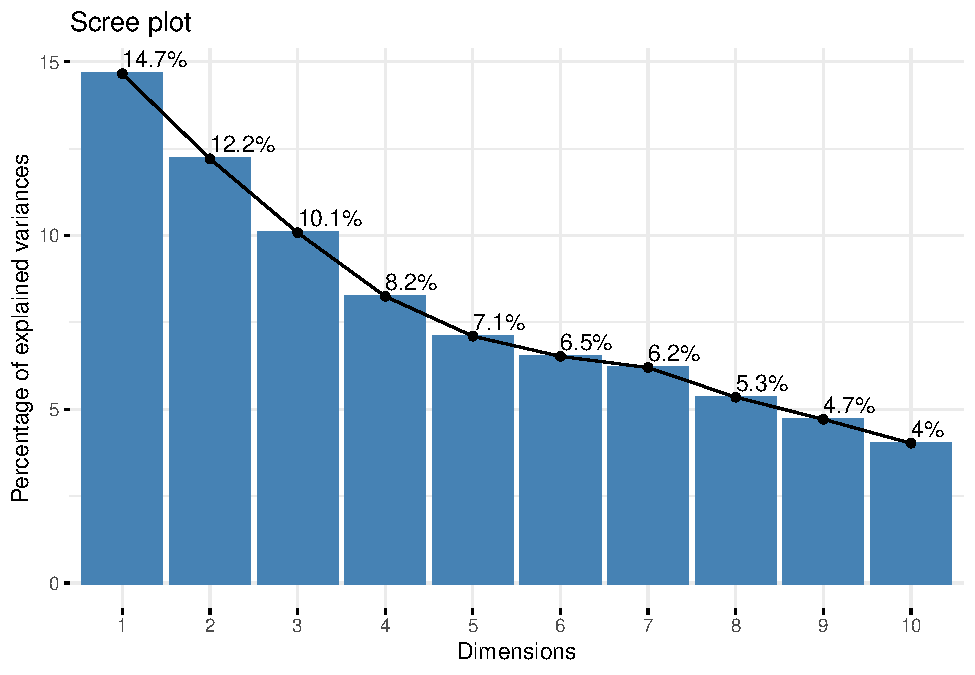
\includegraphics{Average-User-MCA_files/figure-latex/diet yes not enjoy-1.pdf}

\begin{Shaded}
\begin{Highlighting}[]
\KeywordTok{fviz_mca_var}\NormalTok{(search.MCA, }\DataTypeTok{choice =} \StringTok{"mca.cor"}\NormalTok{, }\DataTypeTok{repel =} \OtherTok{TRUE}\NormalTok{,}
             \DataTypeTok{ggtheme =} \KeywordTok{theme_minimal}\NormalTok{())}
\end{Highlighting}
\end{Shaded}

\begin{verbatim}
## Warning: ggrepel: 23 unlabeled data points (too many overlaps). Consider
## increasing max.overlaps
\end{verbatim}

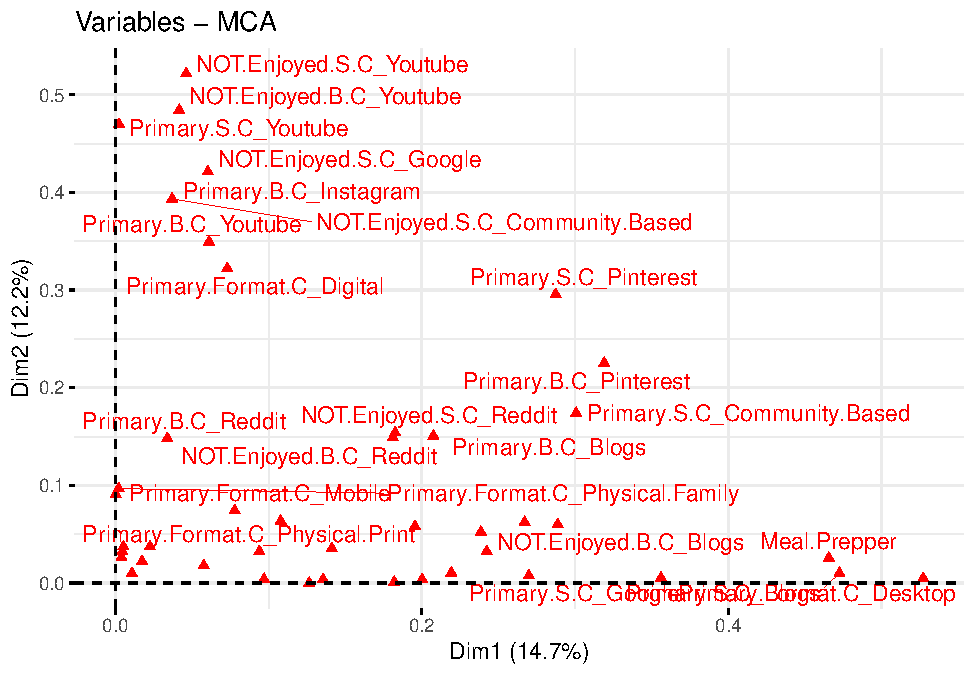
\includegraphics{Average-User-MCA_files/figure-latex/diet yes not enjoy-2.pdf}

\begin{Shaded}
\begin{Highlighting}[]
\KeywordTok{fviz_mca_var}\NormalTok{(search.MCA, }\DataTypeTok{col.var =} \StringTok{"cos2"}\NormalTok{,}
             \DataTypeTok{gradient.cols =} \KeywordTok{c}\NormalTok{(}\StringTok{"#00AFBB"}\NormalTok{, }\StringTok{"#E7B800"}\NormalTok{, }\StringTok{"#FC4E07"}\NormalTok{),}
             \DataTypeTok{repel =} \OtherTok{TRUE}\NormalTok{, }\DataTypeTok{ggtheme =} \KeywordTok{theme_minimal}\NormalTok{())}
\end{Highlighting}
\end{Shaded}

\begin{verbatim}
## Warning: ggrepel: 97 unlabeled data points (too many overlaps). Consider
## increasing max.overlaps
\end{verbatim}

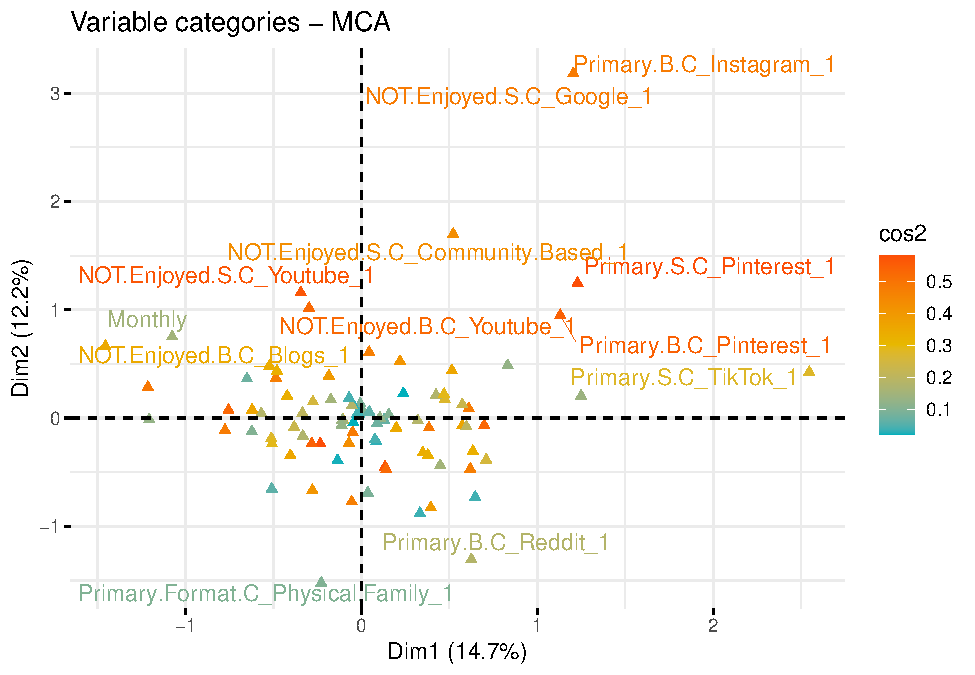
\includegraphics{Average-User-MCA_files/figure-latex/diet yes not enjoy-3.pdf}

\begin{Shaded}
\begin{Highlighting}[]
\NormalTok{NOT.enjoyed.data<-cleaned.Diet.No[}\KeywordTok{c}\NormalTok{(}\StringTok{"Age"}\NormalTok{, }\StringTok{"Meal.Prepper"}\NormalTok{,}\StringTok{"Home.Cook.Rate"}\NormalTok{,}\StringTok{"Primary.Format.C"}\NormalTok{,}\StringTok{"Primary.S.C"}\NormalTok{,}
            \StringTok{"NOT.Enjoyed.S.C"}\NormalTok{,}\StringTok{"Primary.B.C"}\NormalTok{,}\StringTok{"NOT.Enjoyed.B.C"}\NormalTok{,}\StringTok{"Ing.L.V.Above"}\NormalTok{,}
            \StringTok{"Ing.L.Com.Inline.V.Below"}\NormalTok{,}\StringTok{"Ing.Above.Com.Below.V.Inline"}\NormalTok{,  }\StringTok{"Ing.By.Step.V.Above"}\NormalTok{,  }\StringTok{"Ing.By.Step.V.Scroll.L"}\NormalTok{,}
            \StringTok{"Ing.Above.V.Scroll.L"}\NormalTok{)]}

\NormalTok{NOT.enjoyed.data.clean<-}\KeywordTok{cleaner.S}\NormalTok{(NOT.enjoyed.data)}
\NormalTok{search.MCA=}\KeywordTok{MCA}\NormalTok{(NOT.enjoyed.data.clean,}\DataTypeTok{graph=}\OtherTok{FALSE}\NormalTok{)}
\KeywordTok{fviz_screeplot}\NormalTok{(search.MCA,}\DataTypeTok{addlabels=}\NormalTok{T)}
\end{Highlighting}
\end{Shaded}

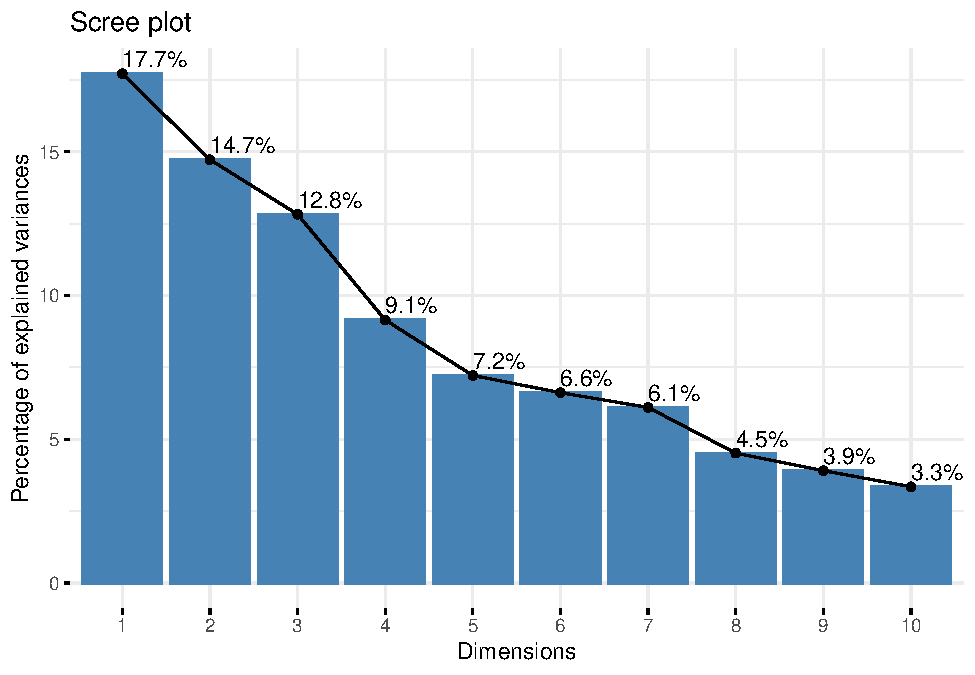
\includegraphics{Average-User-MCA_files/figure-latex/diet no not enjoyed-1.pdf}

\begin{Shaded}
\begin{Highlighting}[]
\KeywordTok{fviz_mca_var}\NormalTok{(search.MCA, }\DataTypeTok{choice =} \StringTok{"mca.cor"}\NormalTok{, }\DataTypeTok{repel =} \OtherTok{TRUE}\NormalTok{,}
             \DataTypeTok{ggtheme =} \KeywordTok{theme_minimal}\NormalTok{())}
\end{Highlighting}
\end{Shaded}

\begin{verbatim}
## Warning: ggrepel: 29 unlabeled data points (too many overlaps). Consider
## increasing max.overlaps
\end{verbatim}

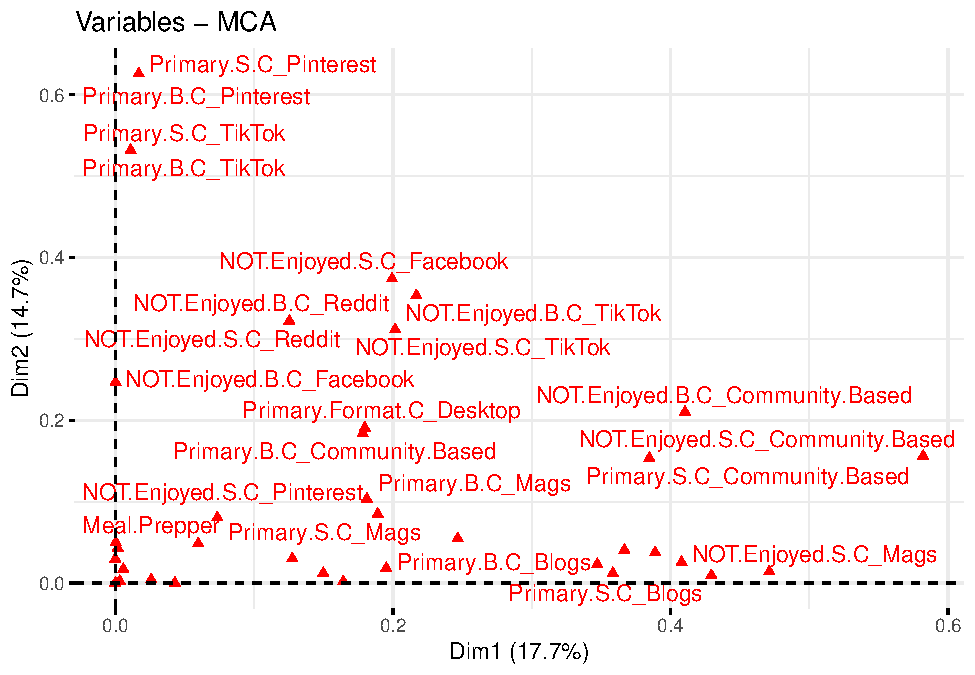
\includegraphics{Average-User-MCA_files/figure-latex/diet no not enjoyed-2.pdf}

\begin{Shaded}
\begin{Highlighting}[]
\KeywordTok{fviz_mca_var}\NormalTok{(search.MCA, }\DataTypeTok{col.var =} \StringTok{"cos2"}\NormalTok{,}
             \DataTypeTok{gradient.cols =} \KeywordTok{c}\NormalTok{(}\StringTok{"#00AFBB"}\NormalTok{, }\StringTok{"#E7B800"}\NormalTok{, }\StringTok{"#FC4E07"}\NormalTok{),}
             \DataTypeTok{repel =} \OtherTok{TRUE}\NormalTok{, }\DataTypeTok{ggtheme =} \KeywordTok{theme_minimal}\NormalTok{())}
\end{Highlighting}
\end{Shaded}

\begin{verbatim}
## Warning: ggrepel: 92 unlabeled data points (too many overlaps). Consider
## increasing max.overlaps
\end{verbatim}

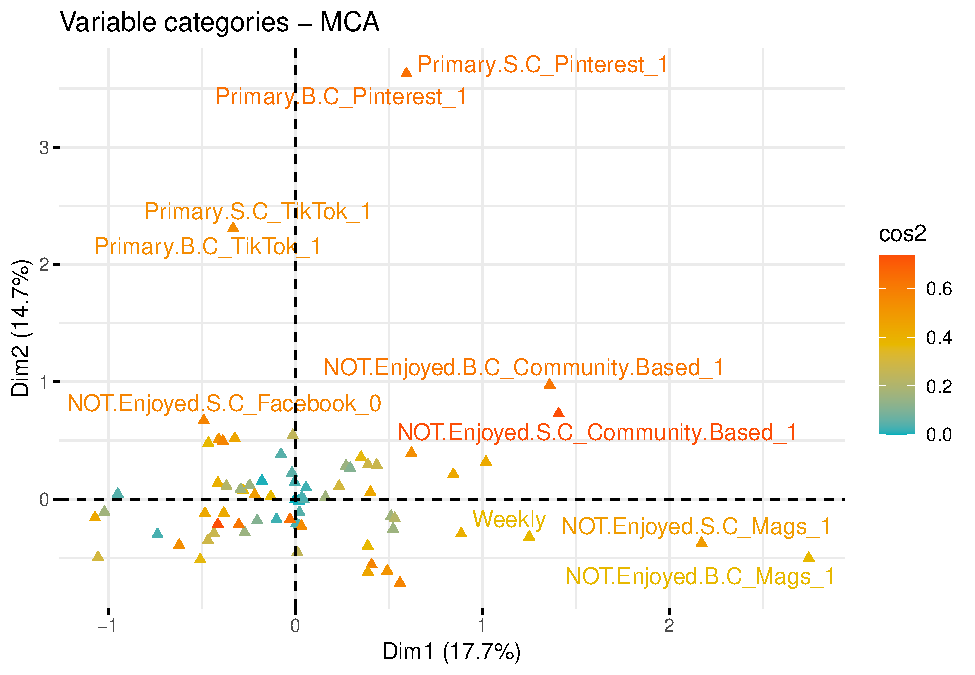
\includegraphics{Average-User-MCA_files/figure-latex/diet no not enjoyed-3.pdf}

\hypertarget{searching-1}{%
\subsubsection{Searching?}\label{searching-1}}

\begin{Shaded}
\begin{Highlighting}[]
\NormalTok{searching.data<-cleaned.Diet.Yes[}\KeywordTok{c}\NormalTok{(}\StringTok{"Age"}\NormalTok{, }\StringTok{"Meal.Prepper"}\NormalTok{,}\StringTok{"Home.Cook.Rate"}\NormalTok{,}\StringTok{"Primary.Format.C"}\NormalTok{,}\StringTok{"Primary.S.C"}\NormalTok{,}
            \StringTok{"Enjoyed.S.C"}\NormalTok{,}\StringTok{"NOT.Enjoyed.S.C"}\NormalTok{,}\StringTok{"Recipe.Search.F"}\NormalTok{,}\StringTok{"Repeat.S.F"}\NormalTok{,}\StringTok{"Browse.Search.F"}\NormalTok{,}\StringTok{"Click.Rate"}\NormalTok{,}
            \StringTok{"Search.Browse.Same"}\NormalTok{, }\StringTok{"Influential.R.C"}\NormalTok{,}\StringTok{"Seek.R.F"}\NormalTok{, }\StringTok{"Save.F"}\NormalTok{,}\StringTok{"Save.C"}\NormalTok{,}\StringTok{"Ing.L.V.Above"}\NormalTok{,}
            \StringTok{"Ing.L.Com.Inline.V.Below"}\NormalTok{,}\StringTok{"Ing.Above.Com.Below.V.Inline"}\NormalTok{,  }\StringTok{"Ing.By.Step.V.Above"}\NormalTok{,  }\StringTok{"Ing.By.Step.V.Scroll.L"}\NormalTok{,}
            \StringTok{"Ing.Above.V.Scroll.L"}\NormalTok{)]}

\NormalTok{searching.data.clean<-}\KeywordTok{cleaner.S}\NormalTok{(searching.data)}
\NormalTok{search.MCA=}\KeywordTok{MCA}\NormalTok{(searching.data.clean,}\DataTypeTok{graph=}\OtherTok{FALSE}\NormalTok{)}
\KeywordTok{fviz_screeplot}\NormalTok{(search.MCA,}\DataTypeTok{addlabels=}\NormalTok{T)}
\end{Highlighting}
\end{Shaded}

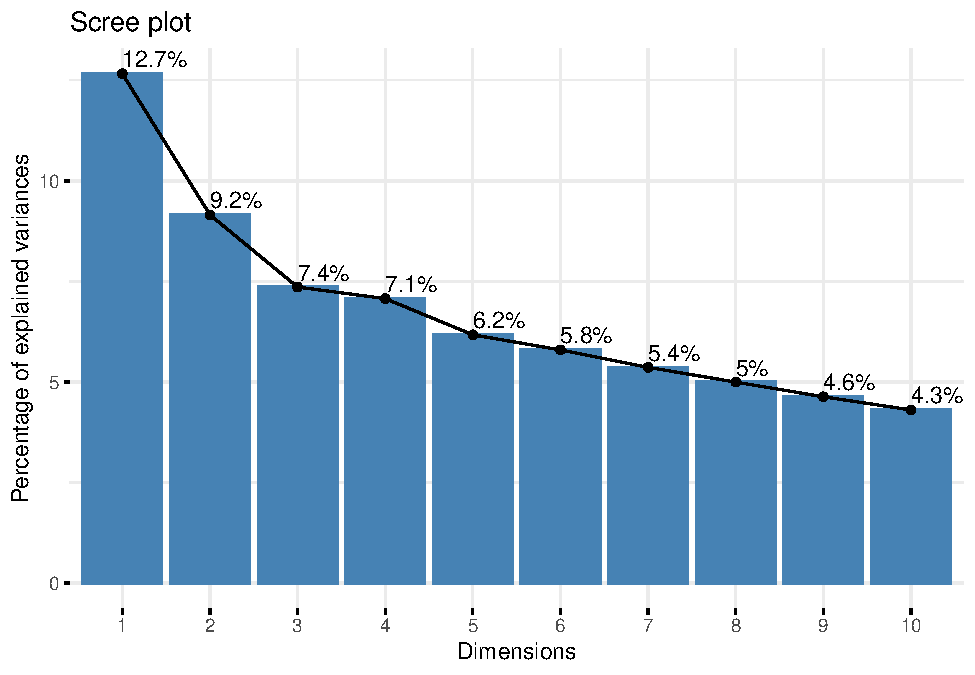
\includegraphics{Average-User-MCA_files/figure-latex/diet yes search-1.pdf}

\begin{Shaded}
\begin{Highlighting}[]
\KeywordTok{fviz_mca_var}\NormalTok{(search.MCA, }\DataTypeTok{choice =} \StringTok{"mca.cor"}\NormalTok{, }\DataTypeTok{repel =} \OtherTok{TRUE}\NormalTok{,}
             \DataTypeTok{ggtheme =} \KeywordTok{theme_minimal}\NormalTok{())}
\end{Highlighting}
\end{Shaded}

\begin{verbatim}
## Warning: ggrepel: 33 unlabeled data points (too many overlaps). Consider
## increasing max.overlaps
\end{verbatim}

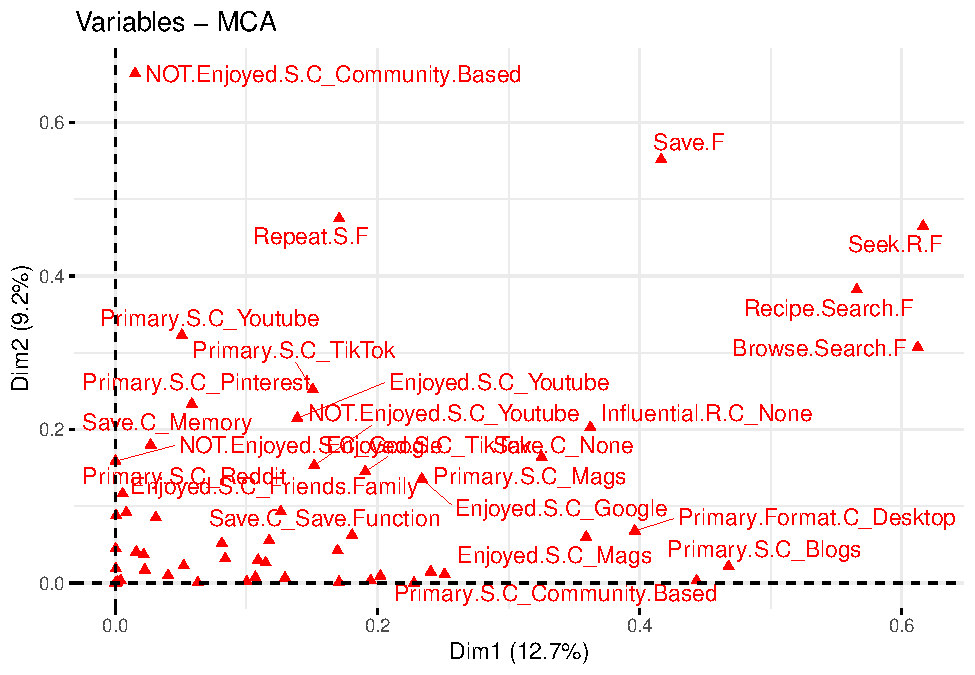
\includegraphics{Average-User-MCA_files/figure-latex/diet yes search-2.pdf}

\begin{Shaded}
\begin{Highlighting}[]
\KeywordTok{fviz_mca_var}\NormalTok{(search.MCA, }\DataTypeTok{col.var =} \StringTok{"cos2"}\NormalTok{,}
             \DataTypeTok{gradient.cols =} \KeywordTok{c}\NormalTok{(}\StringTok{"#00AFBB"}\NormalTok{, }\StringTok{"#E7B800"}\NormalTok{, }\StringTok{"#FC4E07"}\NormalTok{),}
             \DataTypeTok{repel =} \OtherTok{TRUE}\NormalTok{, }\DataTypeTok{ggtheme =} \KeywordTok{theme_minimal}\NormalTok{())}
\end{Highlighting}
\end{Shaded}

\begin{verbatim}
## Warning: ggrepel: 129 unlabeled data points (too many overlaps). Consider
## increasing max.overlaps
\end{verbatim}

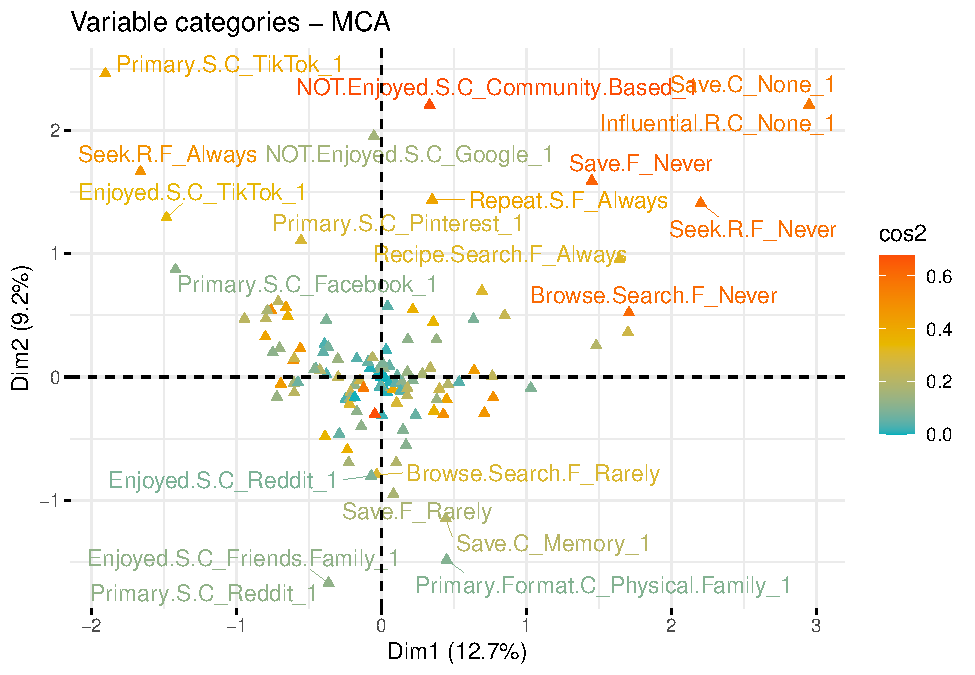
\includegraphics{Average-User-MCA_files/figure-latex/diet yes search-3.pdf}

\begin{Shaded}
\begin{Highlighting}[]
\NormalTok{searching.data<-cleaned.Diet.No[}\KeywordTok{c}\NormalTok{(}\StringTok{"Age"}\NormalTok{, }\StringTok{"Meal.Prepper"}\NormalTok{,}\StringTok{"Home.Cook.Rate"}\NormalTok{,}\StringTok{"Primary.Format.C"}\NormalTok{,}\StringTok{"Primary.S.C"}\NormalTok{,}
            \StringTok{"Enjoyed.S.C"}\NormalTok{,}\StringTok{"NOT.Enjoyed.S.C"}\NormalTok{,}\StringTok{"Recipe.Search.F"}\NormalTok{,}\StringTok{"Repeat.S.F"}\NormalTok{,}\StringTok{"Browse.Search.F"}\NormalTok{,}\StringTok{"Click.Rate"}\NormalTok{,}
            \StringTok{"Search.Browse.Same"}\NormalTok{, }\StringTok{"Influential.R.C"}\NormalTok{,}\StringTok{"Seek.R.F"}\NormalTok{, }\StringTok{"Save.F"}\NormalTok{,}\StringTok{"Save.C"}\NormalTok{,}\StringTok{"Ing.L.V.Above"}\NormalTok{,}
            \StringTok{"Ing.L.Com.Inline.V.Below"}\NormalTok{,}\StringTok{"Ing.Above.Com.Below.V.Inline"}\NormalTok{,  }\StringTok{"Ing.By.Step.V.Above"}\NormalTok{,  }\StringTok{"Ing.By.Step.V.Scroll.L"}\NormalTok{,}
            \StringTok{"Ing.Above.V.Scroll.L"}\NormalTok{)]}

\NormalTok{searching.data.clean<-}\KeywordTok{cleaner.S}\NormalTok{(searching.data)}
\NormalTok{search.MCA=}\KeywordTok{MCA}\NormalTok{(searching.data.clean,}\DataTypeTok{graph=}\OtherTok{FALSE}\NormalTok{)}
\KeywordTok{fviz_screeplot}\NormalTok{(search.MCA,}\DataTypeTok{addlabels=}\NormalTok{T)}
\end{Highlighting}
\end{Shaded}

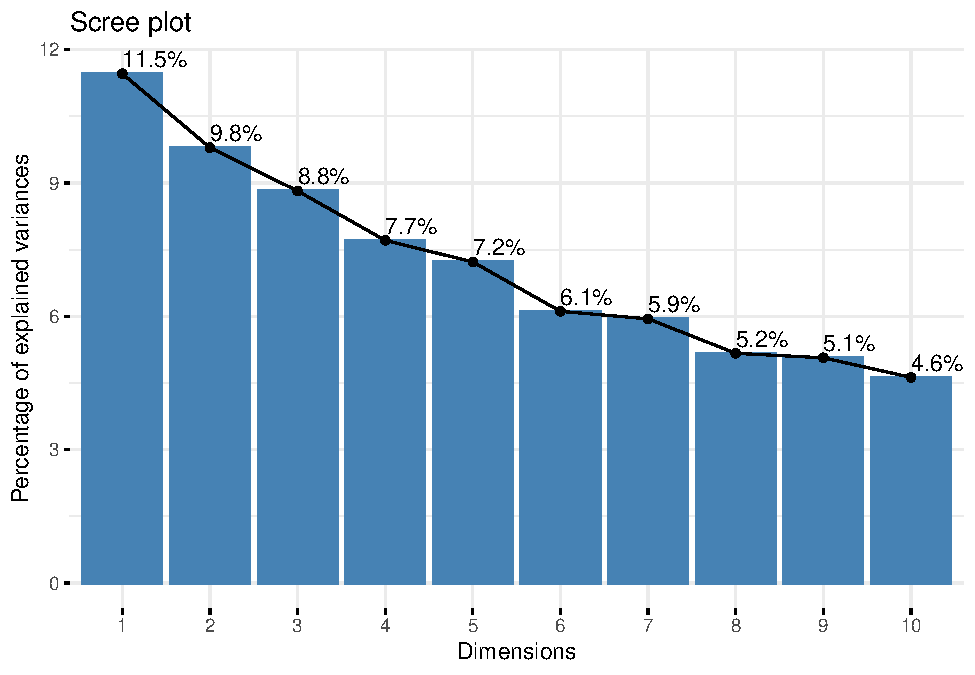
\includegraphics{Average-User-MCA_files/figure-latex/diet no search-1.pdf}

\begin{Shaded}
\begin{Highlighting}[]
\KeywordTok{fviz_mca_var}\NormalTok{(search.MCA, }\DataTypeTok{choice =} \StringTok{"mca.cor"}\NormalTok{, }\DataTypeTok{repel =} \OtherTok{TRUE}\NormalTok{,}
             \DataTypeTok{ggtheme =} \KeywordTok{theme_minimal}\NormalTok{())}
\end{Highlighting}
\end{Shaded}

\begin{verbatim}
## Warning: ggrepel: 36 unlabeled data points (too many overlaps). Consider
## increasing max.overlaps
\end{verbatim}

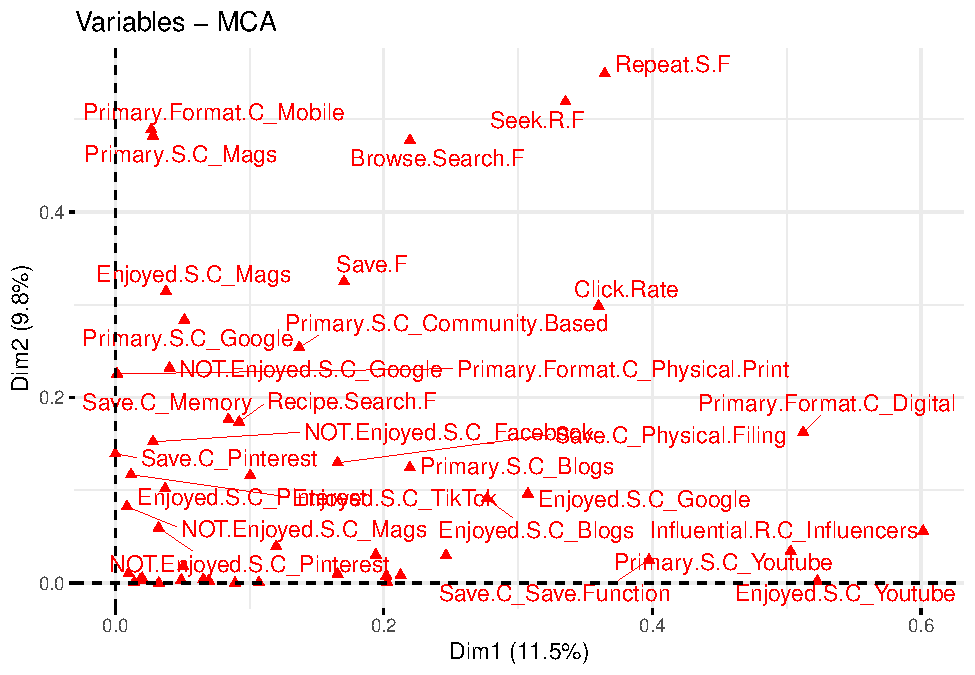
\includegraphics{Average-User-MCA_files/figure-latex/diet no search-2.pdf}

\begin{Shaded}
\begin{Highlighting}[]
\KeywordTok{fviz_mca_var}\NormalTok{(search.MCA, }\DataTypeTok{col.var =} \StringTok{"cos2"}\NormalTok{,}
             \DataTypeTok{gradient.cols =} \KeywordTok{c}\NormalTok{(}\StringTok{"#00AFBB"}\NormalTok{, }\StringTok{"#E7B800"}\NormalTok{, }\StringTok{"#FC4E07"}\NormalTok{),}
             \DataTypeTok{repel =} \OtherTok{TRUE}\NormalTok{, }\DataTypeTok{ggtheme =} \KeywordTok{theme_minimal}\NormalTok{())}
\end{Highlighting}
\end{Shaded}

\begin{verbatim}
## Warning: ggrepel: 133 unlabeled data points (too many overlaps). Consider
## increasing max.overlaps
\end{verbatim}

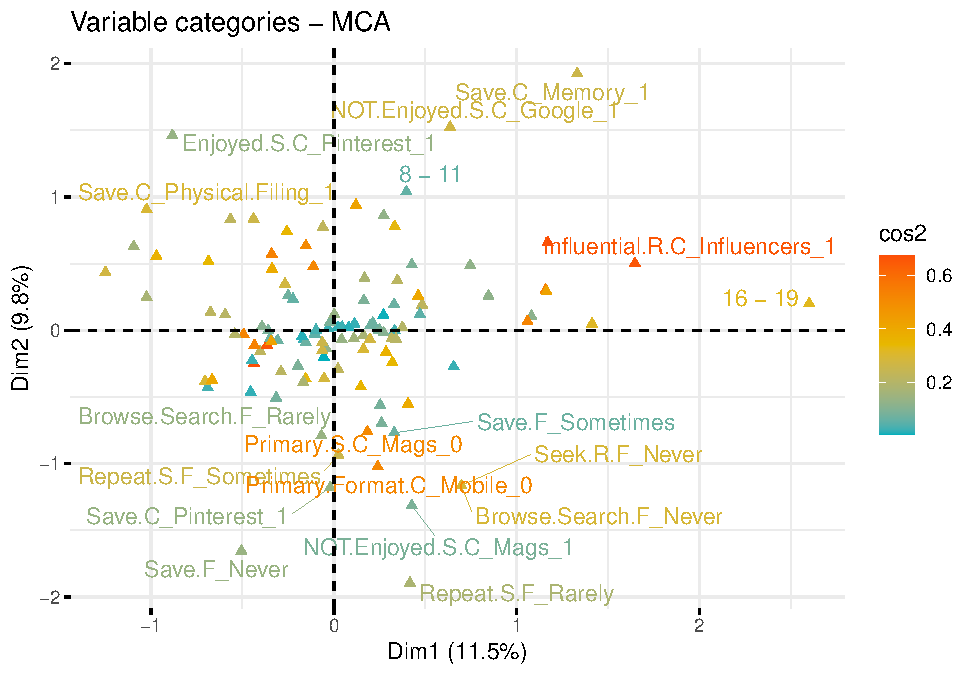
\includegraphics{Average-User-MCA_files/figure-latex/diet no search-3.pdf}

\hypertarget{browsing-1}{%
\subsubsection{Browsing?}\label{browsing-1}}

\begin{Shaded}
\begin{Highlighting}[]
\NormalTok{searching.data<-cleaned.Diet.Yes[}\KeywordTok{c}\NormalTok{(}\StringTok{"Age"}\NormalTok{, }\StringTok{"Meal.Prepper"}\NormalTok{,}\StringTok{"Home.Cook.Rate"}\NormalTok{,}\StringTok{"Primary.Format.C"}\NormalTok{,}\StringTok{"Browse.Search.F"}\NormalTok{,}
            \StringTok{"Search.Browse.Same"}\NormalTok{,}\StringTok{"Primary.B.C"}\NormalTok{,}\StringTok{"Enjoyed.B.C"}\NormalTok{,}\StringTok{"NOT.Enjoyed.B.C"}\NormalTok{,}\StringTok{"Ing.L.V.Above"}\NormalTok{,}
            \StringTok{"Ing.L.Com.Inline.V.Below"}\NormalTok{,}\StringTok{"Ing.Above.Com.Below.V.Inline"}\NormalTok{,  }\StringTok{"Ing.By.Step.V.Above"}\NormalTok{,  }\StringTok{"Ing.By.Step.V.Scroll.L"}\NormalTok{,}
            \StringTok{"Ing.Above.V.Scroll.L"}\NormalTok{)]}

\NormalTok{searching.data.clean<-}\KeywordTok{cleaner.S}\NormalTok{(searching.data)}
\NormalTok{search.MCA=}\KeywordTok{MCA}\NormalTok{(searching.data.clean,}\DataTypeTok{graph=}\OtherTok{FALSE}\NormalTok{)}
\KeywordTok{fviz_screeplot}\NormalTok{(search.MCA,}\DataTypeTok{addlabels=}\NormalTok{T)}
\end{Highlighting}
\end{Shaded}

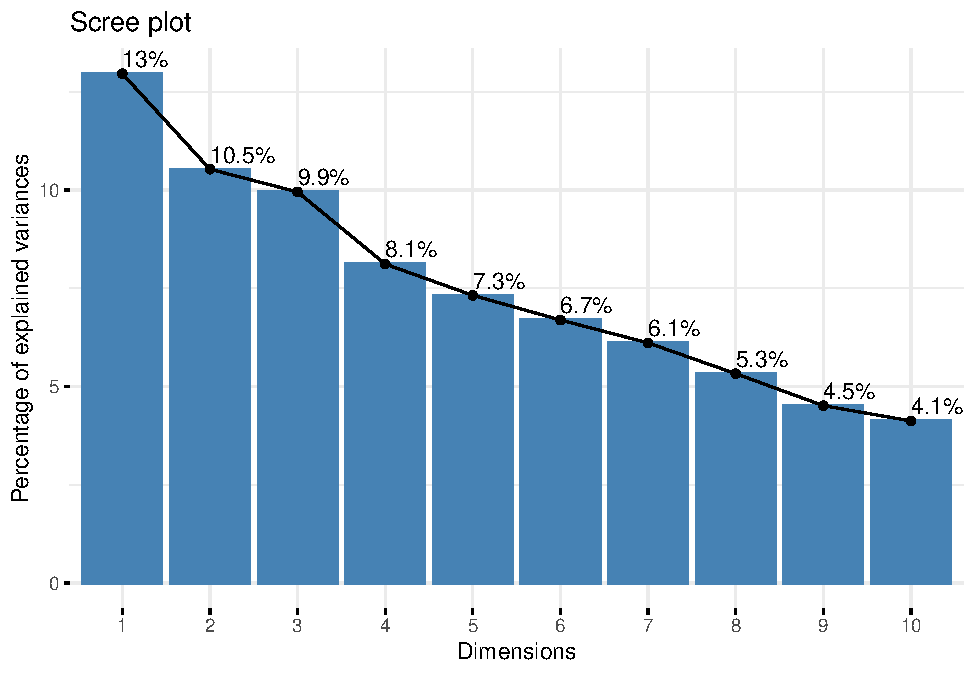
\includegraphics{Average-User-MCA_files/figure-latex/diet yes browse-1.pdf}

\begin{Shaded}
\begin{Highlighting}[]
\KeywordTok{fviz_mca_var}\NormalTok{(search.MCA, }\DataTypeTok{choice =} \StringTok{"mca.cor"}\NormalTok{, }\DataTypeTok{repel =} \OtherTok{TRUE}\NormalTok{,}
             \DataTypeTok{ggtheme =} \KeywordTok{theme_minimal}\NormalTok{())}
\end{Highlighting}
\end{Shaded}

\begin{verbatim}
## Warning: ggrepel: 16 unlabeled data points (too many overlaps). Consider
## increasing max.overlaps
\end{verbatim}

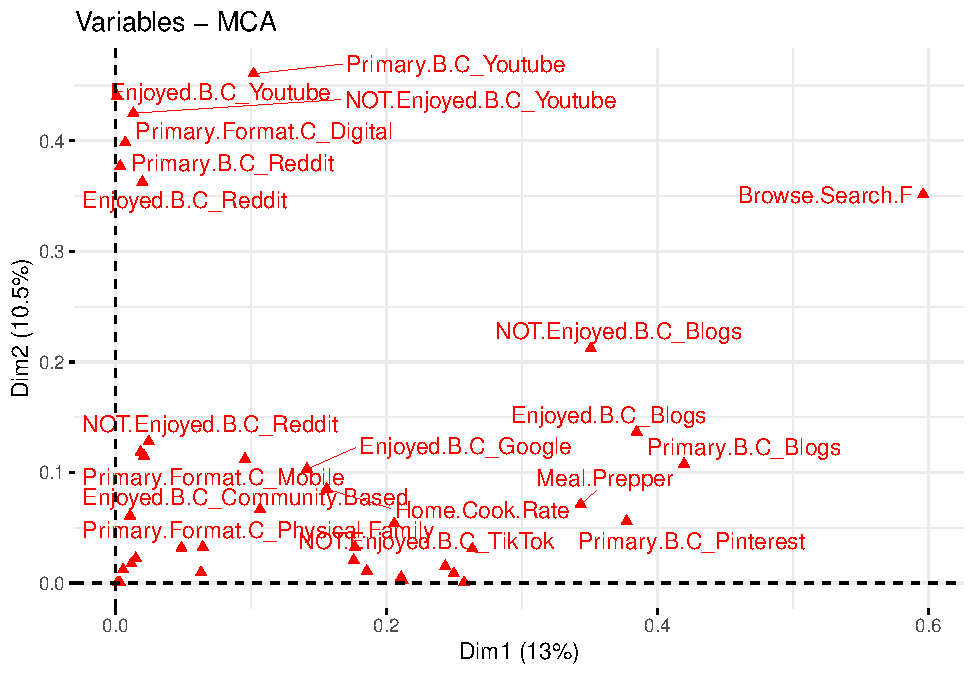
\includegraphics{Average-User-MCA_files/figure-latex/diet yes browse-2.pdf}

\begin{Shaded}
\begin{Highlighting}[]
\KeywordTok{fviz_mca_var}\NormalTok{(search.MCA, }\DataTypeTok{col.var =} \StringTok{"cos2"}\NormalTok{,}
             \DataTypeTok{gradient.cols =} \KeywordTok{c}\NormalTok{(}\StringTok{"#00AFBB"}\NormalTok{, }\StringTok{"#E7B800"}\NormalTok{, }\StringTok{"#FC4E07"}\NormalTok{),}
             \DataTypeTok{repel =} \OtherTok{TRUE}\NormalTok{, }\DataTypeTok{ggtheme =} \KeywordTok{theme_minimal}\NormalTok{())}
\end{Highlighting}
\end{Shaded}

\begin{verbatim}
## Warning: ggrepel: 83 unlabeled data points (too many overlaps). Consider
## increasing max.overlaps
\end{verbatim}

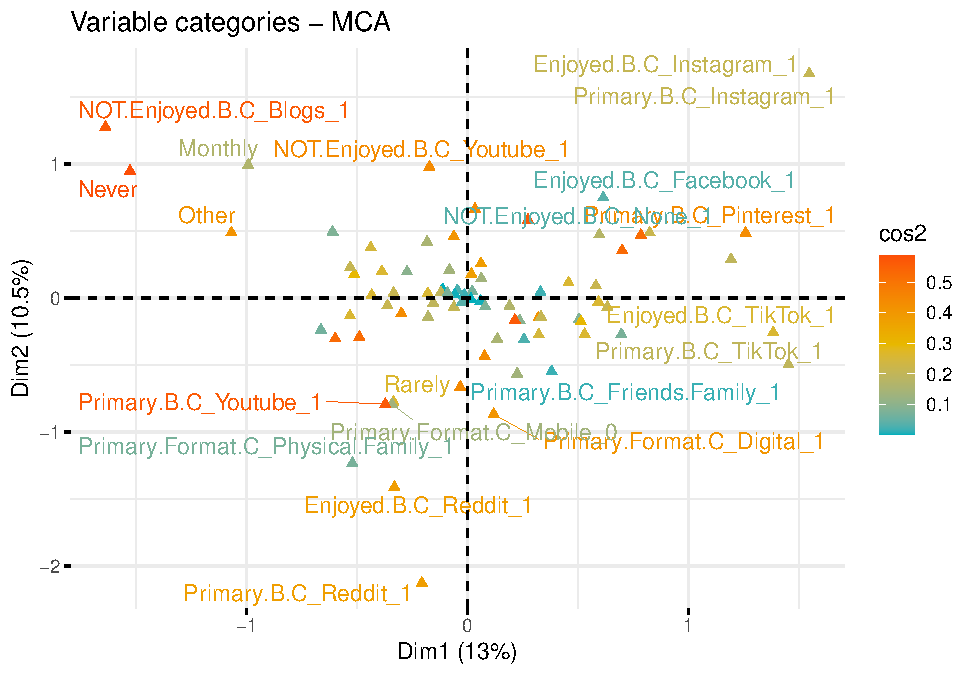
\includegraphics{Average-User-MCA_files/figure-latex/diet yes browse-3.pdf}

\begin{Shaded}
\begin{Highlighting}[]
\NormalTok{searching.data<-cleaned.Diet.No[}\KeywordTok{c}\NormalTok{(}\StringTok{"Age"}\NormalTok{, }\StringTok{"Meal.Prepper"}\NormalTok{,}\StringTok{"Home.Cook.Rate"}\NormalTok{,}\StringTok{"Primary.Format.C"}\NormalTok{,}\StringTok{"Browse.Search.F"}\NormalTok{,}
            \StringTok{"Search.Browse.Same"}\NormalTok{,}\StringTok{"Primary.B.C"}\NormalTok{,}\StringTok{"Enjoyed.B.C"}\NormalTok{,}\StringTok{"NOT.Enjoyed.B.C"}\NormalTok{,}\StringTok{"Ing.L.V.Above"}\NormalTok{,}
            \StringTok{"Ing.L.Com.Inline.V.Below"}\NormalTok{,}\StringTok{"Ing.Above.Com.Below.V.Inline"}\NormalTok{,  }\StringTok{"Ing.By.Step.V.Above"}\NormalTok{,  }\StringTok{"Ing.By.Step.V.Scroll.L"}\NormalTok{,}
            \StringTok{"Ing.Above.V.Scroll.L"}\NormalTok{)]}

\NormalTok{searching.data.clean<-}\KeywordTok{cleaner.S}\NormalTok{(searching.data)}
\NormalTok{search.MCA=}\KeywordTok{MCA}\NormalTok{(searching.data.clean,}\DataTypeTok{graph=}\OtherTok{FALSE}\NormalTok{)}
\KeywordTok{fviz_screeplot}\NormalTok{(search.MCA,}\DataTypeTok{addlabels=}\NormalTok{T)}
\end{Highlighting}
\end{Shaded}

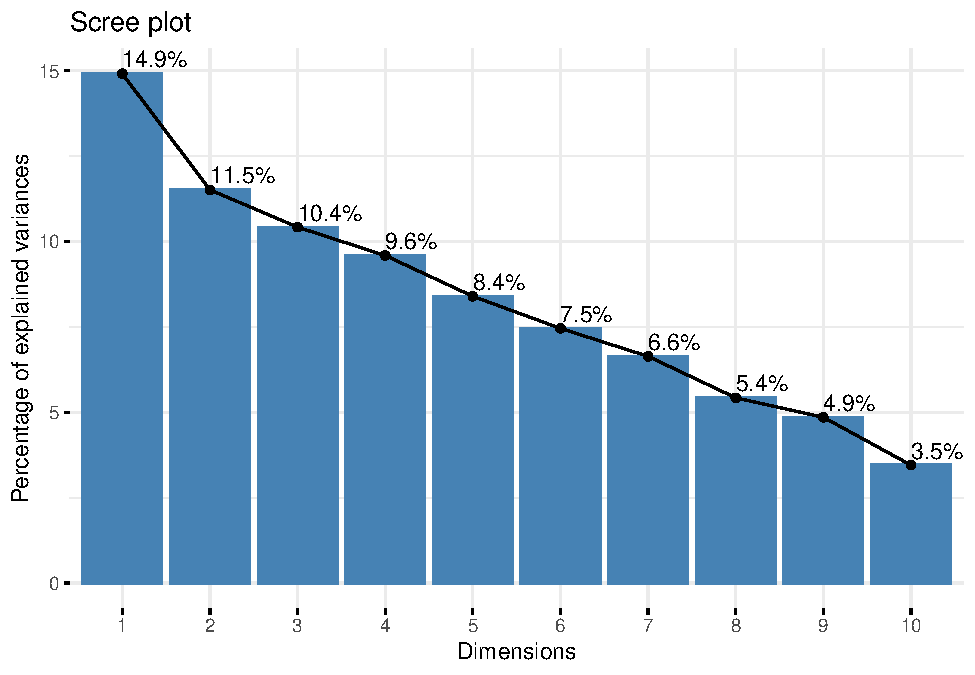
\includegraphics{Average-User-MCA_files/figure-latex/diet no browse-1.pdf}

\begin{Shaded}
\begin{Highlighting}[]
\KeywordTok{fviz_mca_var}\NormalTok{(search.MCA, }\DataTypeTok{choice =} \StringTok{"mca.cor"}\NormalTok{, }\DataTypeTok{repel =} \OtherTok{TRUE}\NormalTok{,}
             \DataTypeTok{ggtheme =} \KeywordTok{theme_minimal}\NormalTok{())}
\end{Highlighting}
\end{Shaded}

\begin{verbatim}
## Warning: ggrepel: 10 unlabeled data points (too many overlaps). Consider
## increasing max.overlaps
\end{verbatim}

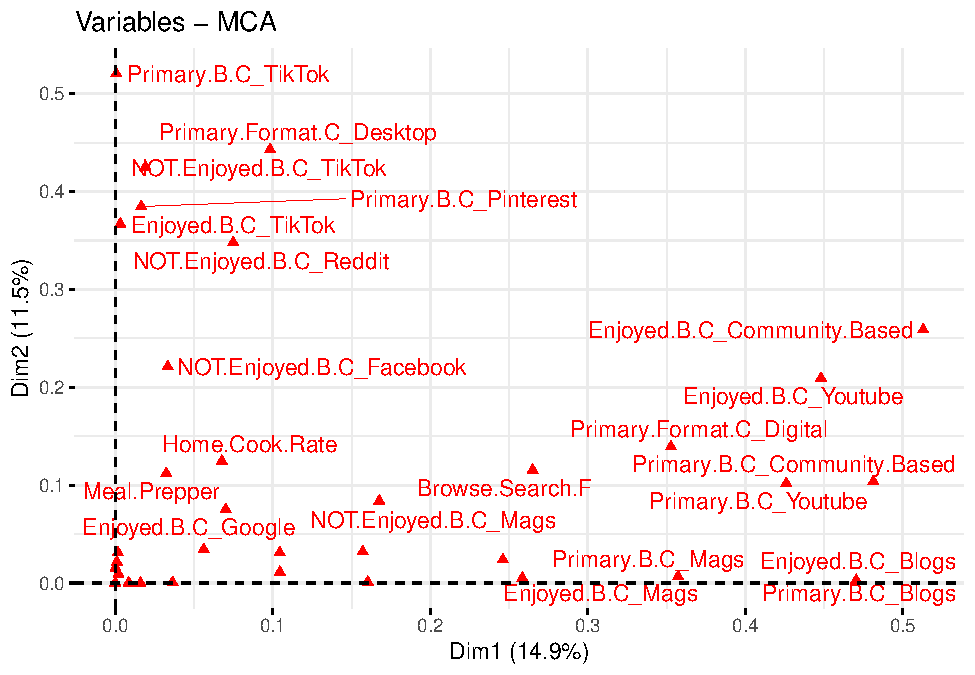
\includegraphics{Average-User-MCA_files/figure-latex/diet no browse-2.pdf}

\begin{Shaded}
\begin{Highlighting}[]
\KeywordTok{fviz_mca_var}\NormalTok{(search.MCA, }\DataTypeTok{col.var =} \StringTok{"cos2"}\NormalTok{,}
             \DataTypeTok{gradient.cols =} \KeywordTok{c}\NormalTok{(}\StringTok{"#00AFBB"}\NormalTok{, }\StringTok{"#E7B800"}\NormalTok{, }\StringTok{"#FC4E07"}\NormalTok{),}
             \DataTypeTok{repel =} \OtherTok{TRUE}\NormalTok{, }\DataTypeTok{ggtheme =} \KeywordTok{theme_minimal}\NormalTok{())}
\end{Highlighting}
\end{Shaded}

\begin{verbatim}
## Warning: ggrepel: 83 unlabeled data points (too many overlaps). Consider
## increasing max.overlaps
\end{verbatim}

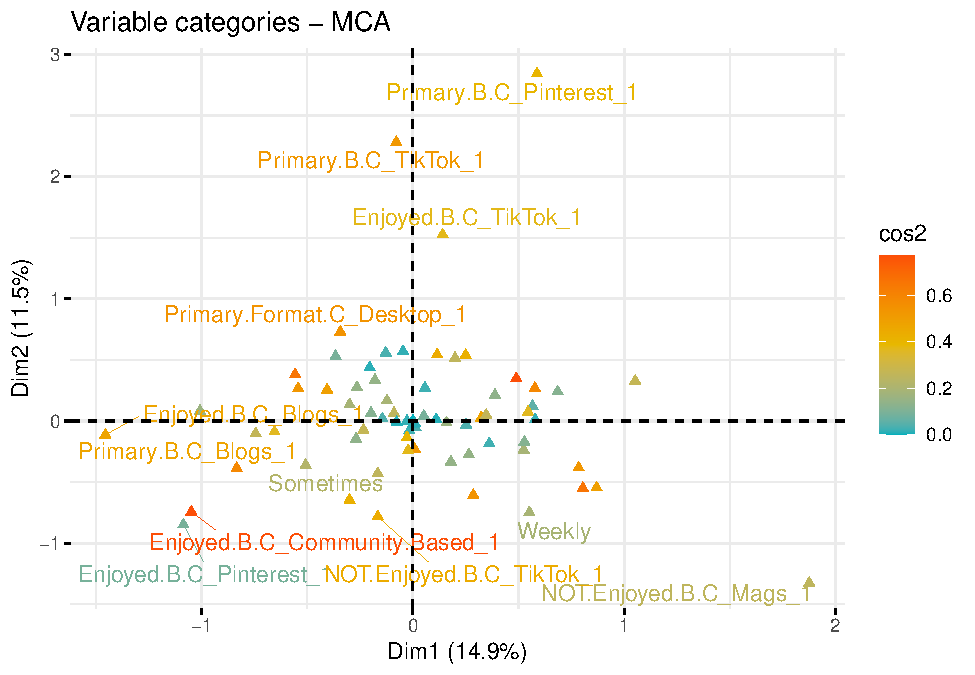
\includegraphics{Average-User-MCA_files/figure-latex/diet no browse-3.pdf}

\hypertarget{review-discuss-1}{%
\subsubsection{Review \& Discuss?}\label{review-discuss-1}}

\begin{Shaded}
\begin{Highlighting}[]
\NormalTok{discussion.data<-cleaned.Diet.Yes[}\KeywordTok{c}\NormalTok{(}\StringTok{"Age"}\NormalTok{, }\StringTok{"Meal.Prepper"}\NormalTok{,}\StringTok{"Home.Cook.Rate"}\NormalTok{,}\StringTok{"Primary.Format.C"}\NormalTok{,}\StringTok{"Primary.R.C"}\NormalTok{, }\StringTok{"Influential.R.C"}\NormalTok{, }
            \StringTok{"Use.R.F"}\NormalTok{,}\StringTok{"Seek.R.F"}\NormalTok{, }\StringTok{"R.F"}\NormalTok{,}\StringTok{"Disc.F"}\NormalTok{,}\StringTok{"Read.Disc.F"}\NormalTok{,}\StringTok{"Disc.C"}\NormalTok{,}\StringTok{"Enjoy.Disc.C"}\NormalTok{,}\StringTok{"Ing.L.V.Above"}\NormalTok{,}
            \StringTok{"Ing.L.Com.Inline.V.Below"}\NormalTok{,}\StringTok{"Ing.Above.Com.Below.V.Inline"}\NormalTok{,  }\StringTok{"Ing.By.Step.V.Above"}\NormalTok{,  }\StringTok{"Ing.By.Step.V.Scroll.L"}\NormalTok{,}
            \StringTok{"Ing.Above.V.Scroll.L"}\NormalTok{)]}

\NormalTok{discussion.data.clean<-}\KeywordTok{cleaner.S}\NormalTok{(discussion.data)}
\NormalTok{search.MCA=}\KeywordTok{MCA}\NormalTok{(discussion.data.clean,}\DataTypeTok{graph=}\OtherTok{FALSE}\NormalTok{)}
\KeywordTok{fviz_screeplot}\NormalTok{(search.MCA,}\DataTypeTok{addlabels=}\NormalTok{T)}
\end{Highlighting}
\end{Shaded}

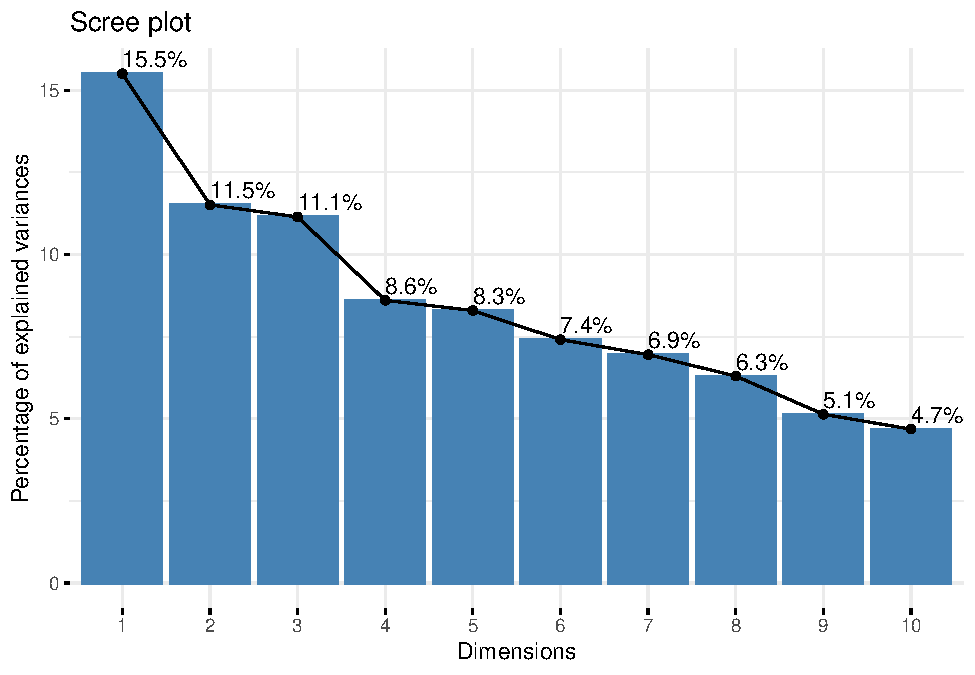
\includegraphics{Average-User-MCA_files/figure-latex/diet yes social-1.pdf}

\begin{Shaded}
\begin{Highlighting}[]
\KeywordTok{fviz_mca_var}\NormalTok{(search.MCA, }\DataTypeTok{choice =} \StringTok{"mca.cor"}\NormalTok{, }\DataTypeTok{repel =} \OtherTok{TRUE}\NormalTok{,}
             \DataTypeTok{ggtheme =} \KeywordTok{theme_minimal}\NormalTok{())}
\end{Highlighting}
\end{Shaded}

\begin{verbatim}
## Warning: ggrepel: 28 unlabeled data points (too many overlaps). Consider
## increasing max.overlaps
\end{verbatim}

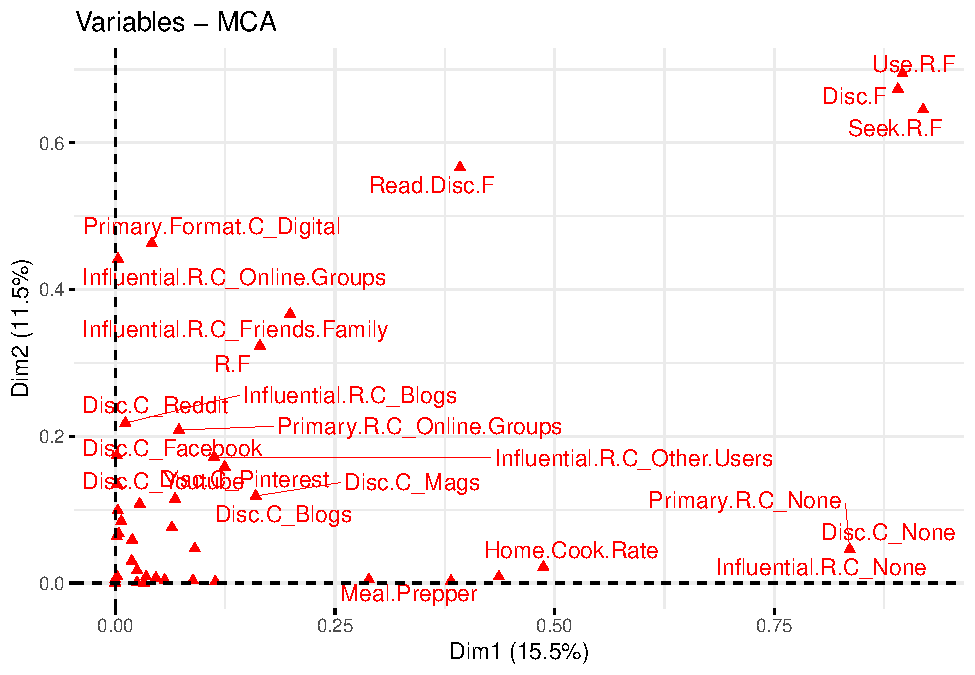
\includegraphics{Average-User-MCA_files/figure-latex/diet yes social-2.pdf}

\begin{Shaded}
\begin{Highlighting}[]
\KeywordTok{fviz_mca_var}\NormalTok{(search.MCA, }\DataTypeTok{col.var =} \StringTok{"cos2"}\NormalTok{,}
             \DataTypeTok{gradient.cols =} \KeywordTok{c}\NormalTok{(}\StringTok{"#00AFBB"}\NormalTok{, }\StringTok{"#E7B800"}\NormalTok{, }\StringTok{"#FC4E07"}\NormalTok{),}
             \DataTypeTok{repel =} \OtherTok{TRUE}\NormalTok{, }\DataTypeTok{ggtheme =} \KeywordTok{theme_minimal}\NormalTok{())}
\end{Highlighting}
\end{Shaded}

\begin{verbatim}
## Warning: ggrepel: 100 unlabeled data points (too many overlaps). Consider
## increasing max.overlaps
\end{verbatim}

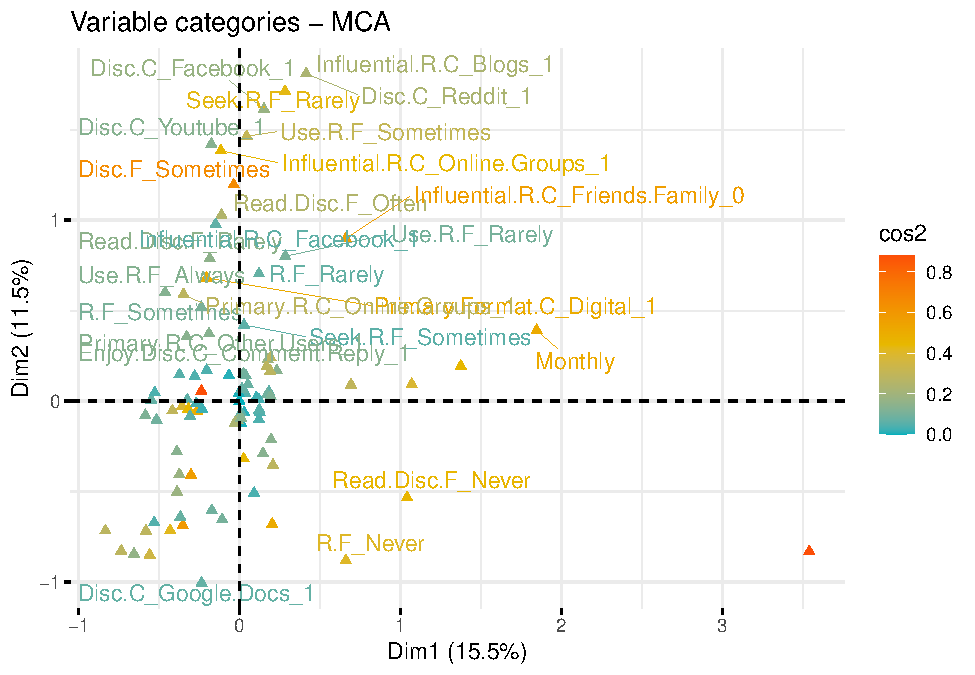
\includegraphics{Average-User-MCA_files/figure-latex/diet yes social-3.pdf}

\begin{Shaded}
\begin{Highlighting}[]
\NormalTok{discussion.data<-cleaned.Diet.No[}\KeywordTok{c}\NormalTok{(}\StringTok{"Age"}\NormalTok{, }\StringTok{"Meal.Prepper"}\NormalTok{,}\StringTok{"Home.Cook.Rate"}\NormalTok{,}\StringTok{"Primary.Format.C"}\NormalTok{,}\StringTok{"Primary.R.C"}\NormalTok{, }\StringTok{"Influential.R.C"}\NormalTok{, }
            \StringTok{"Use.R.F"}\NormalTok{,}\StringTok{"Seek.R.F"}\NormalTok{, }\StringTok{"R.F"}\NormalTok{,}\StringTok{"Disc.F"}\NormalTok{,}\StringTok{"Read.Disc.F"}\NormalTok{,}\StringTok{"Disc.C"}\NormalTok{,}\StringTok{"Enjoy.Disc.C"}\NormalTok{,}\StringTok{"Ing.L.V.Above"}\NormalTok{,}
            \StringTok{"Ing.L.Com.Inline.V.Below"}\NormalTok{,}\StringTok{"Ing.Above.Com.Below.V.Inline"}\NormalTok{,  }\StringTok{"Ing.By.Step.V.Above"}\NormalTok{,  }\StringTok{"Ing.By.Step.V.Scroll.L"}\NormalTok{,}
            \StringTok{"Ing.Above.V.Scroll.L"}\NormalTok{)]}

\NormalTok{discussion.data.clean<-}\KeywordTok{cleaner.S}\NormalTok{(discussion.data)}
\NormalTok{search.MCA=}\KeywordTok{MCA}\NormalTok{(discussion.data.clean,}\DataTypeTok{graph=}\OtherTok{FALSE}\NormalTok{)}
\KeywordTok{fviz_screeplot}\NormalTok{(search.MCA,}\DataTypeTok{addlabels=}\NormalTok{T)}
\end{Highlighting}
\end{Shaded}

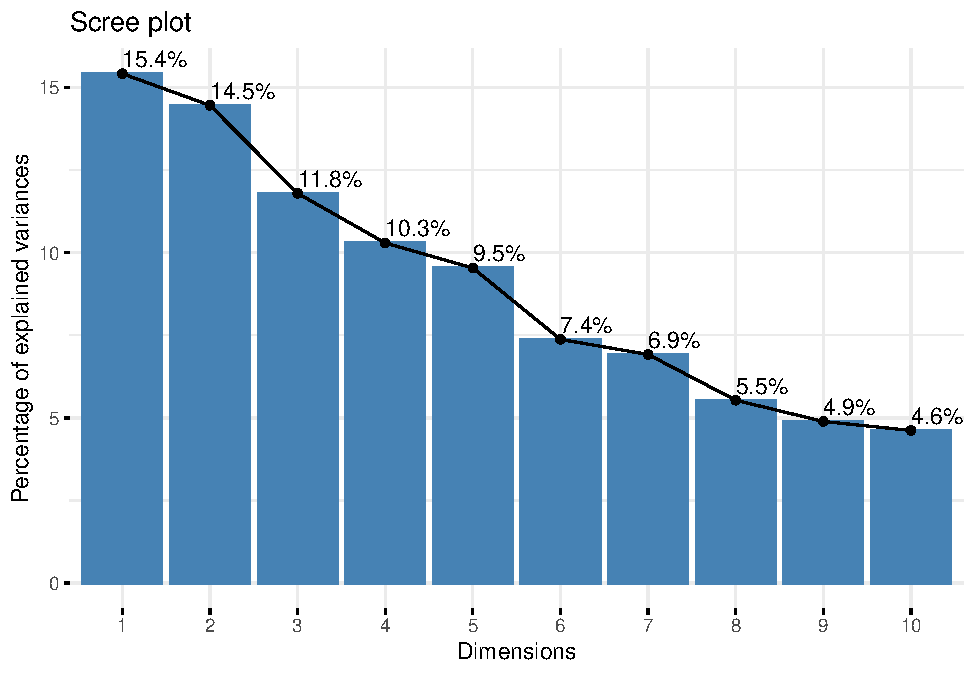
\includegraphics{Average-User-MCA_files/figure-latex/diet no social-1.pdf}

\begin{Shaded}
\begin{Highlighting}[]
\KeywordTok{fviz_mca_var}\NormalTok{(search.MCA, }\DataTypeTok{choice =} \StringTok{"mca.cor"}\NormalTok{, }\DataTypeTok{repel =} \OtherTok{TRUE}\NormalTok{,}
             \DataTypeTok{ggtheme =} \KeywordTok{theme_minimal}\NormalTok{())}
\end{Highlighting}
\end{Shaded}

\begin{verbatim}
## Warning: ggrepel: 20 unlabeled data points (too many overlaps). Consider
## increasing max.overlaps
\end{verbatim}

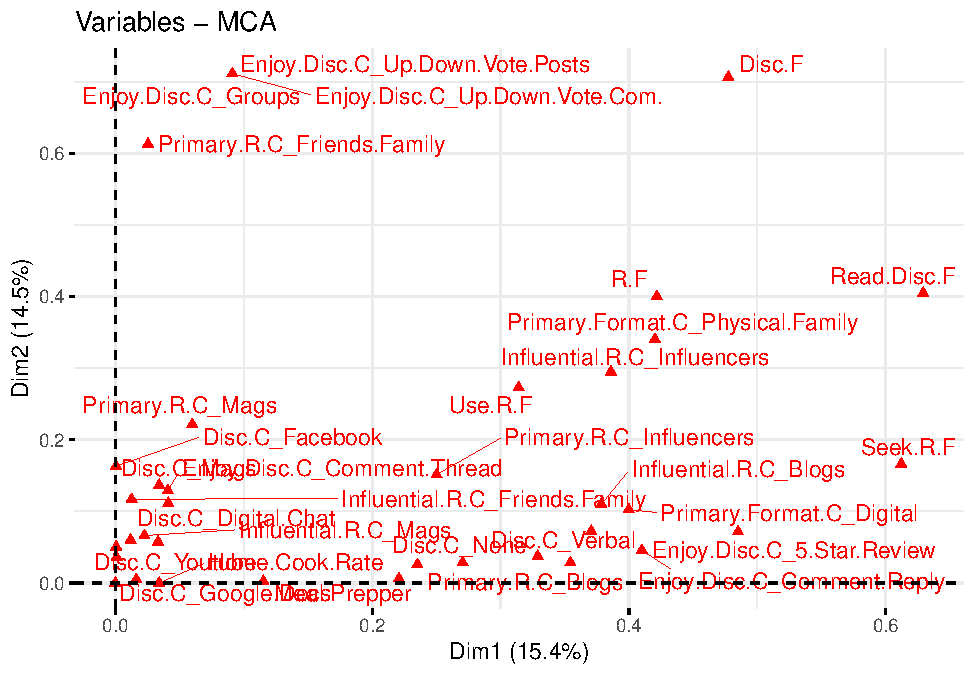
\includegraphics{Average-User-MCA_files/figure-latex/diet no social-2.pdf}

\begin{Shaded}
\begin{Highlighting}[]
\KeywordTok{fviz_mca_var}\NormalTok{(search.MCA, }\DataTypeTok{col.var =} \StringTok{"cos2"}\NormalTok{,}
             \DataTypeTok{gradient.cols =} \KeywordTok{c}\NormalTok{(}\StringTok{"#00AFBB"}\NormalTok{, }\StringTok{"#E7B800"}\NormalTok{, }\StringTok{"#FC4E07"}\NormalTok{),}
             \DataTypeTok{repel =} \OtherTok{TRUE}\NormalTok{, }\DataTypeTok{ggtheme =} \KeywordTok{theme_minimal}\NormalTok{())}
\end{Highlighting}
\end{Shaded}

\begin{verbatim}
## Warning: ggrepel: 113 unlabeled data points (too many overlaps). Consider
## increasing max.overlaps
\end{verbatim}

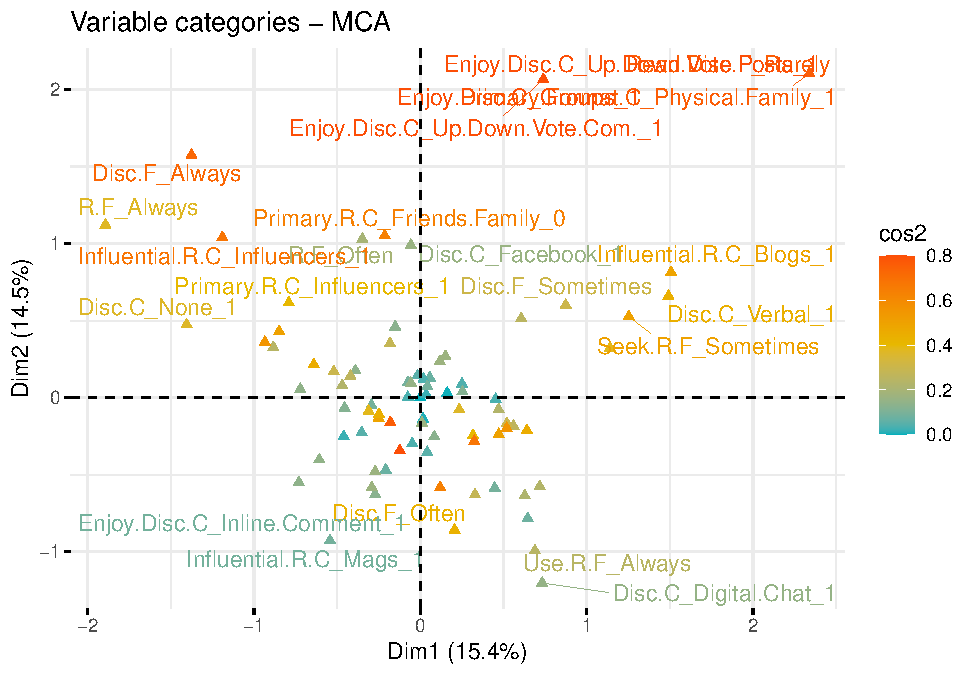
\includegraphics{Average-User-MCA_files/figure-latex/diet no social-3.pdf}
\#\#\# Frequency

\begin{Shaded}
\begin{Highlighting}[]
\NormalTok{freq<-}\StringTok{ }\NormalTok{cleaned.Diet.Yes[}\KeywordTok{c}\NormalTok{(}\StringTok{"Meal.Prepper"}\NormalTok{, }\StringTok{"Age"}\NormalTok{,}\StringTok{"Home.Cook.Rate"}\NormalTok{,}\StringTok{"Recipe.Search.F"}\NormalTok{,}\StringTok{"Repeat.S.F"}\NormalTok{,}\StringTok{"Browse.Search.F"}\NormalTok{,}\StringTok{"Click.Rate"}\NormalTok{,}
            \StringTok{"Use.R.F"}\NormalTok{,}\StringTok{"Seek.R.F"}\NormalTok{, }\StringTok{"R.F"}\NormalTok{,}\StringTok{"Save.F"}\NormalTok{,}\StringTok{"Mod.F"}\NormalTok{, }\StringTok{"Mod.Note.F"}\NormalTok{,}\StringTok{"Disc.F"}\NormalTok{,}\StringTok{"Read.Disc.F"}\NormalTok{,}\StringTok{"Ing.L.V.Above"}\NormalTok{,}
            \StringTok{"Ing.L.Com.Inline.V.Below"}\NormalTok{,}\StringTok{"Ing.Above.Com.Below.V.Inline"}\NormalTok{,  }\StringTok{"Ing.By.Step.V.Above"}\NormalTok{,  }\StringTok{"Ing.By.Step.V.Scroll.L"}\NormalTok{,}
            \StringTok{"Ing.Above.V.Scroll.L"}\NormalTok{)]}
\NormalTok{cols<-}\KeywordTok{names}\NormalTok{(freq)}
\NormalTok{freq<-}\KeywordTok{lapply}\NormalTok{(freq[cols], as.factor)}
\NormalTok{freq<-}\KeywordTok{data.frame}\NormalTok{(freq)}
\NormalTok{search.MCA=}\KeywordTok{MCA}\NormalTok{(freq,}\DataTypeTok{graph=}\OtherTok{FALSE}\NormalTok{)}
\KeywordTok{fviz_screeplot}\NormalTok{(search.MCA,}\DataTypeTok{addlabels=}\NormalTok{T)}
\end{Highlighting}
\end{Shaded}

\includegraphics{Average-User-MCA_files/figure-latex/freq diet yes-1.pdf}

\begin{Shaded}
\begin{Highlighting}[]
\KeywordTok{fviz_mca_var}\NormalTok{(search.MCA, }\DataTypeTok{choice =} \StringTok{"mca.cor"}\NormalTok{, }\DataTypeTok{repel =} \OtherTok{TRUE}\NormalTok{,}
             \DataTypeTok{ggtheme =} \KeywordTok{theme_minimal}\NormalTok{())}
\end{Highlighting}
\end{Shaded}

\includegraphics{Average-User-MCA_files/figure-latex/freq diet yes-2.pdf}

\begin{Shaded}
\begin{Highlighting}[]
\KeywordTok{fviz_mca_var}\NormalTok{(search.MCA, }\DataTypeTok{col.var =} \StringTok{"cos2"}\NormalTok{,}
             \DataTypeTok{gradient.cols =} \KeywordTok{c}\NormalTok{(}\StringTok{"#00AFBB"}\NormalTok{, }\StringTok{"#E7B800"}\NormalTok{, }\StringTok{"#FC4E07"}\NormalTok{),}
             \DataTypeTok{repel =} \OtherTok{TRUE}\NormalTok{, }\DataTypeTok{ggtheme =} \KeywordTok{theme_minimal}\NormalTok{())}
\end{Highlighting}
\end{Shaded}

\begin{verbatim}
## Warning: ggrepel: 50 unlabeled data points (too many overlaps). Consider
## increasing max.overlaps
\end{verbatim}

\includegraphics{Average-User-MCA_files/figure-latex/freq diet yes-3.pdf}

\begin{Shaded}
\begin{Highlighting}[]
\NormalTok{freq<-}\StringTok{ }\NormalTok{cleaned.Diet.No[}\KeywordTok{c}\NormalTok{(}\StringTok{"Meal.Prepper"}\NormalTok{, }\StringTok{"Age"}\NormalTok{,}\StringTok{"Home.Cook.Rate"}\NormalTok{,}\StringTok{"Recipe.Search.F"}\NormalTok{,}\StringTok{"Repeat.S.F"}\NormalTok{,}\StringTok{"Browse.Search.F"}\NormalTok{,}\StringTok{"Click.Rate"}\NormalTok{,}
            \StringTok{"Use.R.F"}\NormalTok{,}\StringTok{"Seek.R.F"}\NormalTok{, }\StringTok{"R.F"}\NormalTok{,}\StringTok{"Save.F"}\NormalTok{,}\StringTok{"Mod.F"}\NormalTok{, }\StringTok{"Mod.Note.F"}\NormalTok{,}\StringTok{"Disc.F"}\NormalTok{,}\StringTok{"Read.Disc.F"}\NormalTok{,}\StringTok{"Ing.L.V.Above"}\NormalTok{,}
            \StringTok{"Ing.L.Com.Inline.V.Below"}\NormalTok{,}\StringTok{"Ing.Above.Com.Below.V.Inline"}\NormalTok{,  }\StringTok{"Ing.By.Step.V.Above"}\NormalTok{,  }\StringTok{"Ing.By.Step.V.Scroll.L"}\NormalTok{,}
            \StringTok{"Ing.Above.V.Scroll.L"}\NormalTok{)]}
\NormalTok{cols<-}\KeywordTok{names}\NormalTok{(freq)}
\NormalTok{freq<-}\KeywordTok{lapply}\NormalTok{(freq[cols], as.factor)}
\NormalTok{freq<-}\KeywordTok{data.frame}\NormalTok{(freq)}
\NormalTok{search.MCA=}\KeywordTok{MCA}\NormalTok{(freq,}\DataTypeTok{graph=}\OtherTok{FALSE}\NormalTok{)}
\KeywordTok{fviz_screeplot}\NormalTok{(search.MCA,}\DataTypeTok{addlabels=}\NormalTok{T)}
\end{Highlighting}
\end{Shaded}

\includegraphics{Average-User-MCA_files/figure-latex/freq diet no-1.pdf}

\begin{Shaded}
\begin{Highlighting}[]
\KeywordTok{fviz_mca_var}\NormalTok{(search.MCA, }\DataTypeTok{choice =} \StringTok{"mca.cor"}\NormalTok{, }\DataTypeTok{repel =} \OtherTok{TRUE}\NormalTok{,}
             \DataTypeTok{ggtheme =} \KeywordTok{theme_minimal}\NormalTok{())}
\end{Highlighting}
\end{Shaded}

\includegraphics{Average-User-MCA_files/figure-latex/freq diet no-2.pdf}

\begin{Shaded}
\begin{Highlighting}[]
\KeywordTok{fviz_mca_var}\NormalTok{(search.MCA, }\DataTypeTok{col.var =} \StringTok{"cos2"}\NormalTok{,}
             \DataTypeTok{gradient.cols =} \KeywordTok{c}\NormalTok{(}\StringTok{"#00AFBB"}\NormalTok{, }\StringTok{"#E7B800"}\NormalTok{, }\StringTok{"#FC4E07"}\NormalTok{),}
             \DataTypeTok{repel =} \OtherTok{TRUE}\NormalTok{, }\DataTypeTok{ggtheme =} \KeywordTok{theme_minimal}\NormalTok{())}
\end{Highlighting}
\end{Shaded}

\begin{verbatim}
## Warning: ggrepel: 75 unlabeled data points (too many overlaps). Consider
## increasing max.overlaps
\end{verbatim}

\includegraphics{Average-User-MCA_files/figure-latex/freq diet no-3.pdf}

\hypertarget{stratify-by-age}{%
\subsection{Stratify by Age}\label{stratify-by-age}}

\begin{Shaded}
\begin{Highlighting}[]
\NormalTok{cleaned.YA<-}\KeywordTok{filter}\NormalTok{(search.data, Age }\OperatorTok{==}\StringTok{ "YA"}\NormalTok{)}
\NormalTok{cleaned.YA<-cleaned.YA}\OperatorTok\KeywordTok{select}\NormalTok{(}\OperatorTok{-}\KeywordTok{c}\NormalTok{(Age))}

\CommentTok{# data.cleaned.YA<-cleaner.S(cleaned.YA)}
\CommentTok{# search.MCA=MCA(data.cleaned.YA,graph=FALSE)}
\CommentTok{# fviz_screeplot(search.MCA,addlabels=T)}
\CommentTok{# fviz_mca_var(search.MCA, choice = "mca.cor", repel = TRUE,}
\CommentTok{#              ggtheme = theme_minimal())}
\CommentTok{# }
\CommentTok{# fviz_mca_var(search.MCA, col.var = "cos2",}
\CommentTok{#              gradient.cols = c("#00AFBB", "#E7B800", "#FC4E07"),}
\CommentTok{#              repel = TRUE, ggtheme = theme_minimal())}
\end{Highlighting}
\end{Shaded}

\begin{Shaded}
\begin{Highlighting}[]
\NormalTok{cleaned.adult<-}\KeywordTok{filter}\NormalTok{(search.data, Age }\OperatorTok{==}\StringTok{ "Adult"}\NormalTok{)}
\NormalTok{cleaned.adult<-cleaned.adult}\OperatorTok\KeywordTok{select}\NormalTok{(}\OperatorTok{-}\KeywordTok{c}\NormalTok{(Age))}

\CommentTok{# data.cleaned.Adult<-cleaner.S(cleaned.adult)}
\CommentTok{# search.MCA=MCA(data.cleaned.Adult,graph=FALSE)}
\CommentTok{# fviz_screeplot(search.MCA,addlabels=T)}
\CommentTok{# fviz_mca_var(search.MCA, choice = "mca.cor", repel = TRUE,}
\CommentTok{#              ggtheme = theme_minimal())}
\CommentTok{# fviz_mca_var(search.MCA, col.var = "cos2",}
\CommentTok{#              gradient.cols = c("#00AFBB", "#E7B800", "#FC4E07"),}
\CommentTok{#              repel = TRUE, ggtheme = theme_minimal())}
\end{Highlighting}
\end{Shaded}

\hypertarget{what-do-users-enjoy-2}{%
\subsubsection{What Do Users Enjoy?}\label{what-do-users-enjoy-2}}

\begin{Shaded}
\begin{Highlighting}[]
\NormalTok{enjoyed.data.YA<-cleaned.YA[}\KeywordTok{c}\NormalTok{(}\StringTok{"Dietary.Restriction"}\NormalTok{, }\StringTok{"Meal.Prepper"}\NormalTok{,}\StringTok{"Home.Cook.Rate"}\NormalTok{,}\StringTok{"Primary.Format.C"}\NormalTok{,}\StringTok{"Primary.S.C"}\NormalTok{,}
            \StringTok{"Enjoyed.S.C"}\NormalTok{,}\StringTok{"NOT.Enjoyed.S.C"}\NormalTok{,}\StringTok{"Primary.B.C"}\NormalTok{,}\StringTok{"Enjoyed.B.C"}\NormalTok{,}\StringTok{"Influential.R.C"}\NormalTok{, }
            \StringTok{"Mod.Note.C"}\NormalTok{, }
            \StringTok{"Note.Method.S"}\NormalTok{,}\StringTok{"Potential.Note.Taker"}\NormalTok{,}\StringTok{"Disc.C"}\NormalTok{,}\StringTok{"Enjoy.Disc.C"}\NormalTok{,}\StringTok{"Ing.L.V.Above"}\NormalTok{,}
            \StringTok{"Ing.L.Com.Inline.V.Below"}\NormalTok{,}\StringTok{"Ing.Above.Com.Below.V.Inline"}\NormalTok{,  }\StringTok{"Ing.By.Step.V.Above"}\NormalTok{,  }\StringTok{"Ing.By.Step.V.Scroll.L"}\NormalTok{,}
            \StringTok{"Ing.Above.V.Scroll.L"}\NormalTok{)]}

\NormalTok{enjoyed.data.clean<-}\KeywordTok{cleaner.S}\NormalTok{(enjoyed.data.YA)}
\NormalTok{search.MCA=}\KeywordTok{MCA}\NormalTok{(enjoyed.data.clean,}\DataTypeTok{graph=}\OtherTok{FALSE}\NormalTok{)}
\KeywordTok{fviz_screeplot}\NormalTok{(search.MCA,}\DataTypeTok{addlabels=}\NormalTok{T)}
\end{Highlighting}
\end{Shaded}

\includegraphics{Average-User-MCA_files/figure-latex/YA enjoy-1.pdf}

\begin{Shaded}
\begin{Highlighting}[]
\KeywordTok{fviz_mca_var}\NormalTok{(search.MCA, }\DataTypeTok{choice =} \StringTok{"mca.cor"}\NormalTok{, }\DataTypeTok{repel =} \OtherTok{TRUE}\NormalTok{,}
             \DataTypeTok{ggtheme =} \KeywordTok{theme_minimal}\NormalTok{())}
\end{Highlighting}
\end{Shaded}

\begin{verbatim}
## Warning: ggrepel: 77 unlabeled data points (too many overlaps). Consider
## increasing max.overlaps
\end{verbatim}

\includegraphics{Average-User-MCA_files/figure-latex/YA enjoy-2.pdf}

\begin{Shaded}
\begin{Highlighting}[]
\KeywordTok{fviz_mca_var}\NormalTok{(search.MCA, }\DataTypeTok{col.var =} \StringTok{"cos2"}\NormalTok{,}
             \DataTypeTok{gradient.cols =} \KeywordTok{c}\NormalTok{(}\StringTok{"#00AFBB"}\NormalTok{, }\StringTok{"#E7B800"}\NormalTok{, }\StringTok{"#FC4E07"}\NormalTok{),}
             \DataTypeTok{repel =} \OtherTok{TRUE}\NormalTok{, }\DataTypeTok{ggtheme =} \KeywordTok{theme_minimal}\NormalTok{())}
\end{Highlighting}
\end{Shaded}

\begin{verbatim}
## Warning: ggrepel: 194 unlabeled data points (too many overlaps). Consider
## increasing max.overlaps
\end{verbatim}

\includegraphics{Average-User-MCA_files/figure-latex/YA enjoy-3.pdf}

\begin{Shaded}
\begin{Highlighting}[]
\NormalTok{enjoyed.data.diet<-cleaned.adult[}\KeywordTok{c}\NormalTok{(}\StringTok{"Dietary.Restriction"}\NormalTok{, }\StringTok{"Meal.Prepper"}\NormalTok{,}\StringTok{"Home.Cook.Rate"}\NormalTok{,}\StringTok{"Primary.Format.C"}\NormalTok{,}\StringTok{"Primary.S.C"}\NormalTok{,}
            \StringTok{"Enjoyed.S.C"}\NormalTok{,}\StringTok{"NOT.Enjoyed.S.C"}\NormalTok{,}\StringTok{"Primary.B.C"}\NormalTok{,}\StringTok{"Enjoyed.B.C"}\NormalTok{,}\StringTok{"Influential.R.C"}\NormalTok{, }
            \StringTok{"Mod.Note.C"}\NormalTok{, }
            \StringTok{"Note.Method.S"}\NormalTok{,}\StringTok{"Potential.Note.Taker"}\NormalTok{,}\StringTok{"Disc.C"}\NormalTok{,}\StringTok{"Enjoy.Disc.C"}\NormalTok{,}\StringTok{"Ing.L.V.Above"}\NormalTok{,}
            \StringTok{"Ing.L.Com.Inline.V.Below"}\NormalTok{,}\StringTok{"Ing.Above.Com.Below.V.Inline"}\NormalTok{,  }\StringTok{"Ing.By.Step.V.Above"}\NormalTok{,  }\StringTok{"Ing.By.Step.V.Scroll.L"}\NormalTok{,}
            \StringTok{"Ing.Above.V.Scroll.L"}\NormalTok{)]}

\NormalTok{enjoyed.data.clean<-}\KeywordTok{cleaner.S}\NormalTok{(enjoyed.data.diet)}
\NormalTok{search.MCA=}\KeywordTok{MCA}\NormalTok{(enjoyed.data.clean,}\DataTypeTok{graph=}\OtherTok{FALSE}\NormalTok{)}
\KeywordTok{fviz_screeplot}\NormalTok{(search.MCA,}\DataTypeTok{addlabels=}\NormalTok{T)}
\end{Highlighting}
\end{Shaded}

\includegraphics{Average-User-MCA_files/figure-latex/adult enjoy-1.pdf}

\begin{Shaded}
\begin{Highlighting}[]
\KeywordTok{fviz_mca_var}\NormalTok{(search.MCA, }\DataTypeTok{choice =} \StringTok{"mca.cor"}\NormalTok{, }\DataTypeTok{repel =} \OtherTok{TRUE}\NormalTok{,}
             \DataTypeTok{ggtheme =} \KeywordTok{theme_minimal}\NormalTok{())}
\end{Highlighting}
\end{Shaded}

\begin{verbatim}
## Warning: ggrepel: 44 unlabeled data points (too many overlaps). Consider
## increasing max.overlaps
\end{verbatim}

\includegraphics{Average-User-MCA_files/figure-latex/adult enjoy-2.pdf}

\begin{Shaded}
\begin{Highlighting}[]
\KeywordTok{fviz_mca_var}\NormalTok{(search.MCA, }\DataTypeTok{col.var =} \StringTok{"cos2"}\NormalTok{,}
             \DataTypeTok{gradient.cols =} \KeywordTok{c}\NormalTok{(}\StringTok{"#00AFBB"}\NormalTok{, }\StringTok{"#E7B800"}\NormalTok{, }\StringTok{"#FC4E07"}\NormalTok{),}
             \DataTypeTok{repel =} \OtherTok{TRUE}\NormalTok{, }\DataTypeTok{ggtheme =} \KeywordTok{theme_minimal}\NormalTok{())}
\end{Highlighting}
\end{Shaded}

\begin{verbatim}
## Warning: ggrepel: 112 unlabeled data points (too many overlaps). Consider
## increasing max.overlaps
\end{verbatim}

\includegraphics{Average-User-MCA_files/figure-latex/adult enjoy-3.pdf}

\hypertarget{what-do-users-not-enjoy-2}{%
\subsubsection{What Do Users NOT
Enjoy?}\label{what-do-users-not-enjoy-2}}

\begin{Shaded}
\begin{Highlighting}[]
\NormalTok{NOT.enjoyed.data<-cleaned.YA[}\KeywordTok{c}\NormalTok{(}\StringTok{"Dietary.Restriction"}\NormalTok{, }\StringTok{"Meal.Prepper"}\NormalTok{,}\StringTok{"Home.Cook.Rate"}\NormalTok{,}\StringTok{"Primary.Format.C"}\NormalTok{,}\StringTok{"Primary.S.C"}\NormalTok{,}
            \StringTok{"NOT.Enjoyed.S.C"}\NormalTok{,}\StringTok{"Primary.B.C"}\NormalTok{,}\StringTok{"NOT.Enjoyed.B.C"}\NormalTok{,}\StringTok{"Ing.L.V.Above"}\NormalTok{,}
            \StringTok{"Ing.L.Com.Inline.V.Below"}\NormalTok{,}\StringTok{"Ing.Above.Com.Below.V.Inline"}\NormalTok{,  }\StringTok{"Ing.By.Step.V.Above"}\NormalTok{,  }\StringTok{"Ing.By.Step.V.Scroll.L"}\NormalTok{,}
            \StringTok{"Ing.Above.V.Scroll.L"}\NormalTok{)]}

\NormalTok{NOT.enjoyed.data.clean<-}\KeywordTok{cleaner.S}\NormalTok{(NOT.enjoyed.data)}
\NormalTok{search.MCA=}\KeywordTok{MCA}\NormalTok{(NOT.enjoyed.data.clean,}\DataTypeTok{graph=}\OtherTok{FALSE}\NormalTok{)}
\KeywordTok{fviz_screeplot}\NormalTok{(search.MCA,}\DataTypeTok{addlabels=}\NormalTok{T)}
\end{Highlighting}
\end{Shaded}

\includegraphics{Average-User-MCA_files/figure-latex/YA not enjoy-1.pdf}

\begin{Shaded}
\begin{Highlighting}[]
\KeywordTok{fviz_mca_var}\NormalTok{(search.MCA, }\DataTypeTok{choice =} \StringTok{"mca.cor"}\NormalTok{, }\DataTypeTok{repel =} \OtherTok{TRUE}\NormalTok{,}
             \DataTypeTok{ggtheme =} \KeywordTok{theme_minimal}\NormalTok{())}
\end{Highlighting}
\end{Shaded}

\begin{verbatim}
## Warning: ggrepel: 18 unlabeled data points (too many overlaps). Consider
## increasing max.overlaps
\end{verbatim}

\includegraphics{Average-User-MCA_files/figure-latex/YA not enjoy-2.pdf}

\begin{Shaded}
\begin{Highlighting}[]
\KeywordTok{fviz_mca_var}\NormalTok{(search.MCA, }\DataTypeTok{col.var =} \StringTok{"cos2"}\NormalTok{,}
             \DataTypeTok{gradient.cols =} \KeywordTok{c}\NormalTok{(}\StringTok{"#00AFBB"}\NormalTok{, }\StringTok{"#E7B800"}\NormalTok{, }\StringTok{"#FC4E07"}\NormalTok{),}
             \DataTypeTok{repel =} \OtherTok{TRUE}\NormalTok{, }\DataTypeTok{ggtheme =} \KeywordTok{theme_minimal}\NormalTok{())}
\end{Highlighting}
\end{Shaded}

\begin{verbatim}
## Warning: ggrepel: 94 unlabeled data points (too many overlaps). Consider
## increasing max.overlaps
\end{verbatim}

\includegraphics{Average-User-MCA_files/figure-latex/YA not enjoy-3.pdf}

\begin{Shaded}
\begin{Highlighting}[]
\NormalTok{NOT.enjoyed.data<-cleaned.adult[}\KeywordTok{c}\NormalTok{(}\StringTok{"Dietary.Restriction"}\NormalTok{, }\StringTok{"Meal.Prepper"}\NormalTok{,}\StringTok{"Home.Cook.Rate"}\NormalTok{,}\StringTok{"Primary.Format.C"}\NormalTok{,}\StringTok{"Primary.S.C"}\NormalTok{,}
            \StringTok{"NOT.Enjoyed.S.C"}\NormalTok{,}\StringTok{"Primary.B.C"}\NormalTok{,}\StringTok{"NOT.Enjoyed.B.C"}\NormalTok{,}\StringTok{"Ing.L.V.Above"}\NormalTok{,}
            \StringTok{"Ing.L.Com.Inline.V.Below"}\NormalTok{,}\StringTok{"Ing.Above.Com.Below.V.Inline"}\NormalTok{,  }\StringTok{"Ing.By.Step.V.Above"}\NormalTok{,  }\StringTok{"Ing.By.Step.V.Scroll.L"}\NormalTok{,}
            \StringTok{"Ing.Above.V.Scroll.L"}\NormalTok{)]}

\NormalTok{NOT.enjoyed.data.clean<-}\KeywordTok{cleaner.S}\NormalTok{(NOT.enjoyed.data)}
\NormalTok{search.MCA=}\KeywordTok{MCA}\NormalTok{(NOT.enjoyed.data.clean,}\DataTypeTok{graph=}\OtherTok{FALSE}\NormalTok{)}
\KeywordTok{fviz_screeplot}\NormalTok{(search.MCA,}\DataTypeTok{addlabels=}\NormalTok{T)}
\end{Highlighting}
\end{Shaded}

\includegraphics{Average-User-MCA_files/figure-latex/adult not enjoyed-1.pdf}

\begin{Shaded}
\begin{Highlighting}[]
\KeywordTok{fviz_mca_var}\NormalTok{(search.MCA, }\DataTypeTok{choice =} \StringTok{"mca.cor"}\NormalTok{, }\DataTypeTok{repel =} \OtherTok{TRUE}\NormalTok{,}
             \DataTypeTok{ggtheme =} \KeywordTok{theme_minimal}\NormalTok{())}
\end{Highlighting}
\end{Shaded}

\begin{verbatim}
## Warning: ggrepel: 22 unlabeled data points (too many overlaps). Consider
## increasing max.overlaps
\end{verbatim}

\includegraphics{Average-User-MCA_files/figure-latex/adult not enjoyed-2.pdf}

\begin{Shaded}
\begin{Highlighting}[]
\KeywordTok{fviz_mca_var}\NormalTok{(search.MCA, }\DataTypeTok{col.var =} \StringTok{"cos2"}\NormalTok{,}
             \DataTypeTok{gradient.cols =} \KeywordTok{c}\NormalTok{(}\StringTok{"#00AFBB"}\NormalTok{, }\StringTok{"#E7B800"}\NormalTok{, }\StringTok{"#FC4E07"}\NormalTok{),}
             \DataTypeTok{repel =} \OtherTok{TRUE}\NormalTok{, }\DataTypeTok{ggtheme =} \KeywordTok{theme_minimal}\NormalTok{())}
\end{Highlighting}
\end{Shaded}

\begin{verbatim}
## Warning: ggrepel: 50 unlabeled data points (too many overlaps). Consider
## increasing max.overlaps
\end{verbatim}

\includegraphics{Average-User-MCA_files/figure-latex/adult not enjoyed-3.pdf}

\hypertarget{searching-2}{%
\subsubsection{Searching?}\label{searching-2}}

\begin{Shaded}
\begin{Highlighting}[]
\NormalTok{searching.data<-cleaned.YA[}\KeywordTok{c}\NormalTok{(}\StringTok{"Dietary.Restriction"}\NormalTok{, }\StringTok{"Meal.Prepper"}\NormalTok{,}\StringTok{"Home.Cook.Rate"}\NormalTok{,}\StringTok{"Primary.Format.C"}\NormalTok{,}\StringTok{"Primary.S.C"}\NormalTok{,}
            \StringTok{"Enjoyed.S.C"}\NormalTok{,}\StringTok{"NOT.Enjoyed.S.C"}\NormalTok{,}\StringTok{"Recipe.Search.F"}\NormalTok{,}\StringTok{"Repeat.S.F"}\NormalTok{,}\StringTok{"Browse.Search.F"}\NormalTok{,}\StringTok{"Click.Rate"}\NormalTok{,}
            \StringTok{"Search.Browse.Same"}\NormalTok{, }\StringTok{"Influential.R.C"}\NormalTok{,}\StringTok{"Seek.R.F"}\NormalTok{, }\StringTok{"Save.F"}\NormalTok{,}\StringTok{"Save.C"}\NormalTok{,}\StringTok{"Ing.L.V.Above"}\NormalTok{,}
            \StringTok{"Ing.L.Com.Inline.V.Below"}\NormalTok{,}\StringTok{"Ing.Above.Com.Below.V.Inline"}\NormalTok{,  }\StringTok{"Ing.By.Step.V.Above"}\NormalTok{,  }\StringTok{"Ing.By.Step.V.Scroll.L"}\NormalTok{,}
            \StringTok{"Ing.Above.V.Scroll.L"}\NormalTok{)]}

\NormalTok{searching.data.clean<-}\KeywordTok{cleaner.S}\NormalTok{(searching.data)}
\NormalTok{search.MCA=}\KeywordTok{MCA}\NormalTok{(searching.data.clean,}\DataTypeTok{graph=}\OtherTok{FALSE}\NormalTok{)}
\KeywordTok{fviz_screeplot}\NormalTok{(search.MCA,}\DataTypeTok{addlabels=}\NormalTok{T)}
\end{Highlighting}
\end{Shaded}

\includegraphics{Average-User-MCA_files/figure-latex/YA search-1.pdf}

\begin{Shaded}
\begin{Highlighting}[]
\KeywordTok{fviz_mca_var}\NormalTok{(search.MCA, }\DataTypeTok{choice =} \StringTok{"mca.cor"}\NormalTok{, }\DataTypeTok{repel =} \OtherTok{TRUE}\NormalTok{,}
             \DataTypeTok{ggtheme =} \KeywordTok{theme_minimal}\NormalTok{())}
\end{Highlighting}
\end{Shaded}

\begin{verbatim}
## Warning: ggrepel: 47 unlabeled data points (too many overlaps). Consider
## increasing max.overlaps
\end{verbatim}

\includegraphics{Average-User-MCA_files/figure-latex/YA search-2.pdf}

\begin{Shaded}
\begin{Highlighting}[]
\KeywordTok{fviz_mca_var}\NormalTok{(search.MCA, }\DataTypeTok{col.var =} \StringTok{"cos2"}\NormalTok{,}
             \DataTypeTok{gradient.cols =} \KeywordTok{c}\NormalTok{(}\StringTok{"#00AFBB"}\NormalTok{, }\StringTok{"#E7B800"}\NormalTok{, }\StringTok{"#FC4E07"}\NormalTok{),}
             \DataTypeTok{repel =} \OtherTok{TRUE}\NormalTok{, }\DataTypeTok{ggtheme =} \KeywordTok{theme_minimal}\NormalTok{())}
\end{Highlighting}
\end{Shaded}

\begin{verbatim}
## Warning: ggrepel: 148 unlabeled data points (too many overlaps). Consider
## increasing max.overlaps
\end{verbatim}

\includegraphics{Average-User-MCA_files/figure-latex/YA search-3.pdf}

\begin{Shaded}
\begin{Highlighting}[]
\NormalTok{searching.data<-cleaned.adult[}\KeywordTok{c}\NormalTok{(}\StringTok{"Dietary.Restriction"}\NormalTok{, }\StringTok{"Meal.Prepper"}\NormalTok{,}\StringTok{"Home.Cook.Rate"}\NormalTok{,}\StringTok{"Primary.Format.C"}\NormalTok{,}\StringTok{"Primary.S.C"}\NormalTok{,}
            \StringTok{"Enjoyed.S.C"}\NormalTok{,}\StringTok{"NOT.Enjoyed.S.C"}\NormalTok{,}\StringTok{"Recipe.Search.F"}\NormalTok{,}\StringTok{"Repeat.S.F"}\NormalTok{,}\StringTok{"Browse.Search.F"}\NormalTok{,}\StringTok{"Click.Rate"}\NormalTok{,}
            \StringTok{"Search.Browse.Same"}\NormalTok{, }\StringTok{"Influential.R.C"}\NormalTok{,}\StringTok{"Seek.R.F"}\NormalTok{, }\StringTok{"Save.F"}\NormalTok{,}\StringTok{"Save.C"}\NormalTok{,}\StringTok{"Ing.L.V.Above"}\NormalTok{,}
            \StringTok{"Ing.L.Com.Inline.V.Below"}\NormalTok{,}\StringTok{"Ing.Above.Com.Below.V.Inline"}\NormalTok{,  }\StringTok{"Ing.By.Step.V.Above"}\NormalTok{,  }\StringTok{"Ing.By.Step.V.Scroll.L"}\NormalTok{,}
            \StringTok{"Ing.Above.V.Scroll.L"}\NormalTok{)]}

\NormalTok{searching.data.clean<-}\KeywordTok{cleaner.S}\NormalTok{(searching.data)}
\NormalTok{search.MCA=}\KeywordTok{MCA}\NormalTok{(searching.data.clean,}\DataTypeTok{graph=}\OtherTok{FALSE}\NormalTok{)}
\KeywordTok{fviz_screeplot}\NormalTok{(search.MCA,}\DataTypeTok{addlabels=}\NormalTok{T)}
\end{Highlighting}
\end{Shaded}

\includegraphics{Average-User-MCA_files/figure-latex/adult search-1.pdf}

\begin{Shaded}
\begin{Highlighting}[]
\KeywordTok{fviz_mca_var}\NormalTok{(search.MCA, }\DataTypeTok{choice =} \StringTok{"mca.cor"}\NormalTok{, }\DataTypeTok{repel =} \OtherTok{TRUE}\NormalTok{,}
             \DataTypeTok{ggtheme =} \KeywordTok{theme_minimal}\NormalTok{())}
\end{Highlighting}
\end{Shaded}

\begin{verbatim}
## Warning: ggrepel: 15 unlabeled data points (too many overlaps). Consider
## increasing max.overlaps
\end{verbatim}

\includegraphics{Average-User-MCA_files/figure-latex/adult search-2.pdf}

\begin{Shaded}
\begin{Highlighting}[]
\KeywordTok{fviz_mca_var}\NormalTok{(search.MCA, }\DataTypeTok{col.var =} \StringTok{"cos2"}\NormalTok{,}
             \DataTypeTok{gradient.cols =} \KeywordTok{c}\NormalTok{(}\StringTok{"#00AFBB"}\NormalTok{, }\StringTok{"#E7B800"}\NormalTok{, }\StringTok{"#FC4E07"}\NormalTok{),}
             \DataTypeTok{repel =} \OtherTok{TRUE}\NormalTok{, }\DataTypeTok{ggtheme =} \KeywordTok{theme_minimal}\NormalTok{())}
\end{Highlighting}
\end{Shaded}

\begin{verbatim}
## Warning: ggrepel: 71 unlabeled data points (too many overlaps). Consider
## increasing max.overlaps
\end{verbatim}

\includegraphics{Average-User-MCA_files/figure-latex/adult search-3.pdf}

\hypertarget{browsing-2}{%
\subsubsection{Browsing?}\label{browsing-2}}

\begin{Shaded}
\begin{Highlighting}[]
\NormalTok{searching.data<-cleaned.YA[}\KeywordTok{c}\NormalTok{(}\StringTok{"Dietary.Restriction"}\NormalTok{, }\StringTok{"Meal.Prepper"}\NormalTok{,}\StringTok{"Home.Cook.Rate"}\NormalTok{,}\StringTok{"Primary.Format.C"}\NormalTok{,}\StringTok{"Browse.Search.F"}\NormalTok{,}
            \StringTok{"Search.Browse.Same"}\NormalTok{,}\StringTok{"Primary.B.C"}\NormalTok{,}\StringTok{"Enjoyed.B.C"}\NormalTok{,}\StringTok{"NOT.Enjoyed.B.C"}\NormalTok{,}\StringTok{"Ing.L.V.Above"}\NormalTok{,}
            \StringTok{"Ing.L.Com.Inline.V.Below"}\NormalTok{,}\StringTok{"Ing.Above.Com.Below.V.Inline"}\NormalTok{,  }\StringTok{"Ing.By.Step.V.Above"}\NormalTok{,  }\StringTok{"Ing.By.Step.V.Scroll.L"}\NormalTok{,}
            \StringTok{"Ing.Above.V.Scroll.L"}\NormalTok{)]}

\NormalTok{searching.data.clean<-}\KeywordTok{cleaner.S}\NormalTok{(searching.data)}
\NormalTok{search.MCA=}\KeywordTok{MCA}\NormalTok{(searching.data.clean,}\DataTypeTok{graph=}\OtherTok{FALSE}\NormalTok{)}
\KeywordTok{fviz_screeplot}\NormalTok{(search.MCA,}\DataTypeTok{addlabels=}\NormalTok{T)}
\end{Highlighting}
\end{Shaded}

\includegraphics{Average-User-MCA_files/figure-latex/YA browse-1.pdf}

\begin{Shaded}
\begin{Highlighting}[]
\KeywordTok{fviz_mca_var}\NormalTok{(search.MCA, }\DataTypeTok{choice =} \StringTok{"mca.cor"}\NormalTok{, }\DataTypeTok{repel =} \OtherTok{TRUE}\NormalTok{,}
             \DataTypeTok{ggtheme =} \KeywordTok{theme_minimal}\NormalTok{())}
\end{Highlighting}
\end{Shaded}

\begin{verbatim}
## Warning: ggrepel: 23 unlabeled data points (too many overlaps). Consider
## increasing max.overlaps
\end{verbatim}

\includegraphics{Average-User-MCA_files/figure-latex/YA browse-2.pdf}

\begin{Shaded}
\begin{Highlighting}[]
\KeywordTok{fviz_mca_var}\NormalTok{(search.MCA, }\DataTypeTok{col.var =} \StringTok{"cos2"}\NormalTok{,}
             \DataTypeTok{gradient.cols =} \KeywordTok{c}\NormalTok{(}\StringTok{"#00AFBB"}\NormalTok{, }\StringTok{"#E7B800"}\NormalTok{, }\StringTok{"#FC4E07"}\NormalTok{),}
             \DataTypeTok{repel =} \OtherTok{TRUE}\NormalTok{, }\DataTypeTok{ggtheme =} \KeywordTok{theme_minimal}\NormalTok{())}
\end{Highlighting}
\end{Shaded}

\begin{verbatim}
## Warning: ggrepel: 88 unlabeled data points (too many overlaps). Consider
## increasing max.overlaps
\end{verbatim}

\includegraphics{Average-User-MCA_files/figure-latex/YA browse-3.pdf}

\begin{Shaded}
\begin{Highlighting}[]
\NormalTok{searching.data<-cleaned.adult[}\KeywordTok{c}\NormalTok{(}\StringTok{"Dietary.Restriction"}\NormalTok{, }\StringTok{"Meal.Prepper"}\NormalTok{,}\StringTok{"Home.Cook.Rate"}\NormalTok{,}\StringTok{"Primary.Format.C"}\NormalTok{,}\StringTok{"Browse.Search.F"}\NormalTok{,}
            \StringTok{"Search.Browse.Same"}\NormalTok{,}\StringTok{"Primary.B.C"}\NormalTok{,}\StringTok{"Enjoyed.B.C"}\NormalTok{,}\StringTok{"NOT.Enjoyed.B.C"}\NormalTok{,}\StringTok{"Ing.L.V.Above"}\NormalTok{,}
            \StringTok{"Ing.L.Com.Inline.V.Below"}\NormalTok{,}\StringTok{"Ing.Above.Com.Below.V.Inline"}\NormalTok{,  }\StringTok{"Ing.By.Step.V.Above"}\NormalTok{,  }\StringTok{"Ing.By.Step.V.Scroll.L"}\NormalTok{,}
            \StringTok{"Ing.Above.V.Scroll.L"}\NormalTok{)]}

\NormalTok{searching.data.clean<-}\KeywordTok{cleaner.S}\NormalTok{(searching.data)}
\NormalTok{search.MCA=}\KeywordTok{MCA}\NormalTok{(searching.data.clean,}\DataTypeTok{graph=}\OtherTok{FALSE}\NormalTok{)}
\KeywordTok{fviz_screeplot}\NormalTok{(search.MCA,}\DataTypeTok{addlabels=}\NormalTok{T)}
\end{Highlighting}
\end{Shaded}

\includegraphics{Average-User-MCA_files/figure-latex/adult browse-1.pdf}

\begin{Shaded}
\begin{Highlighting}[]
\KeywordTok{fviz_mca_var}\NormalTok{(search.MCA, }\DataTypeTok{choice =} \StringTok{"mca.cor"}\NormalTok{, }\DataTypeTok{repel =} \OtherTok{TRUE}\NormalTok{,}
             \DataTypeTok{ggtheme =} \KeywordTok{theme_minimal}\NormalTok{())}
\end{Highlighting}
\end{Shaded}

\begin{verbatim}
## Warning: ggrepel: 17 unlabeled data points (too many overlaps). Consider
## increasing max.overlaps
\end{verbatim}

\includegraphics{Average-User-MCA_files/figure-latex/adult browse-2.pdf}

\begin{Shaded}
\begin{Highlighting}[]
\KeywordTok{fviz_mca_var}\NormalTok{(search.MCA, }\DataTypeTok{col.var =} \StringTok{"cos2"}\NormalTok{,}
             \DataTypeTok{gradient.cols =} \KeywordTok{c}\NormalTok{(}\StringTok{"#00AFBB"}\NormalTok{, }\StringTok{"#E7B800"}\NormalTok{, }\StringTok{"#FC4E07"}\NormalTok{),}
             \DataTypeTok{repel =} \OtherTok{TRUE}\NormalTok{, }\DataTypeTok{ggtheme =} \KeywordTok{theme_minimal}\NormalTok{())}
\end{Highlighting}
\end{Shaded}

\begin{verbatim}
## Warning: ggrepel: 41 unlabeled data points (too many overlaps). Consider
## increasing max.overlaps
\end{verbatim}

\includegraphics{Average-User-MCA_files/figure-latex/adult browse-3.pdf}

\hypertarget{review-discuss-2}{%
\subsubsection{Review \& Discuss?}\label{review-discuss-2}}

\begin{Shaded}
\begin{Highlighting}[]
\NormalTok{discussion.data<-cleaned.YA[}\KeywordTok{c}\NormalTok{(}\StringTok{"Dietary.Restriction"}\NormalTok{, }\StringTok{"Meal.Prepper"}\NormalTok{,}\StringTok{"Home.Cook.Rate"}\NormalTok{,}\StringTok{"Primary.Format.C"}\NormalTok{,}\StringTok{"Primary.R.C"}\NormalTok{, }\StringTok{"Influential.R.C"}\NormalTok{, }
            \StringTok{"Use.R.F"}\NormalTok{,}\StringTok{"Seek.R.F"}\NormalTok{, }\StringTok{"R.F"}\NormalTok{,}\StringTok{"Disc.F"}\NormalTok{,}\StringTok{"Read.Disc.F"}\NormalTok{,}\StringTok{"Disc.C"}\NormalTok{,}\StringTok{"Enjoy.Disc.C"}\NormalTok{,}\StringTok{"Ing.L.V.Above"}\NormalTok{,}
            \StringTok{"Ing.L.Com.Inline.V.Below"}\NormalTok{,}\StringTok{"Ing.Above.Com.Below.V.Inline"}\NormalTok{,  }\StringTok{"Ing.By.Step.V.Above"}\NormalTok{,  }\StringTok{"Ing.By.Step.V.Scroll.L"}\NormalTok{,}
            \StringTok{"Ing.Above.V.Scroll.L"}\NormalTok{)]}

\NormalTok{discussion.data.clean<-}\KeywordTok{cleaner.S}\NormalTok{(discussion.data)}
\NormalTok{search.MCA=}\KeywordTok{MCA}\NormalTok{(discussion.data.clean,}\DataTypeTok{graph=}\OtherTok{FALSE}\NormalTok{)}
\KeywordTok{fviz_screeplot}\NormalTok{(search.MCA,}\DataTypeTok{addlabels=}\NormalTok{T)}
\end{Highlighting}
\end{Shaded}

\includegraphics{Average-User-MCA_files/figure-latex/YA social-1.pdf}

\begin{Shaded}
\begin{Highlighting}[]
\KeywordTok{fviz_mca_var}\NormalTok{(search.MCA, }\DataTypeTok{choice =} \StringTok{"mca.cor"}\NormalTok{, }\DataTypeTok{repel =} \OtherTok{TRUE}\NormalTok{,}
             \DataTypeTok{ggtheme =} \KeywordTok{theme_minimal}\NormalTok{())}
\end{Highlighting}
\end{Shaded}

\begin{verbatim}
## Warning: ggrepel: 39 unlabeled data points (too many overlaps). Consider
## increasing max.overlaps
\end{verbatim}

\includegraphics{Average-User-MCA_files/figure-latex/YA social-2.pdf}

\begin{Shaded}
\begin{Highlighting}[]
\KeywordTok{fviz_mca_var}\NormalTok{(search.MCA, }\DataTypeTok{col.var =} \StringTok{"cos2"}\NormalTok{,}
             \DataTypeTok{gradient.cols =} \KeywordTok{c}\NormalTok{(}\StringTok{"#00AFBB"}\NormalTok{, }\StringTok{"#E7B800"}\NormalTok{, }\StringTok{"#FC4E07"}\NormalTok{),}
             \DataTypeTok{repel =} \OtherTok{TRUE}\NormalTok{, }\DataTypeTok{ggtheme =} \KeywordTok{theme_minimal}\NormalTok{())}
\end{Highlighting}
\end{Shaded}

\begin{verbatim}
## Warning: ggrepel: 118 unlabeled data points (too many overlaps). Consider
## increasing max.overlaps
\end{verbatim}

\includegraphics{Average-User-MCA_files/figure-latex/YA social-3.pdf}

\begin{Shaded}
\begin{Highlighting}[]
\NormalTok{discussion.data<-cleaned.adult[}\KeywordTok{c}\NormalTok{(}\StringTok{"Dietary.Restriction"}\NormalTok{, }\StringTok{"Meal.Prepper"}\NormalTok{,}\StringTok{"Home.Cook.Rate"}\NormalTok{,}\StringTok{"Primary.Format.C"}\NormalTok{,}\StringTok{"Primary.R.C"}\NormalTok{, }\StringTok{"Influential.R.C"}\NormalTok{, }
            \StringTok{"Use.R.F"}\NormalTok{,}\StringTok{"Seek.R.F"}\NormalTok{, }\StringTok{"R.F"}\NormalTok{,}\StringTok{"Disc.F"}\NormalTok{,}\StringTok{"Read.Disc.F"}\NormalTok{,}\StringTok{"Disc.C"}\NormalTok{,}\StringTok{"Enjoy.Disc.C"}\NormalTok{,}\StringTok{"Ing.L.V.Above"}\NormalTok{,}
            \StringTok{"Ing.L.Com.Inline.V.Below"}\NormalTok{,}\StringTok{"Ing.Above.Com.Below.V.Inline"}\NormalTok{,  }\StringTok{"Ing.By.Step.V.Above"}\NormalTok{,  }\StringTok{"Ing.By.Step.V.Scroll.L"}\NormalTok{,}
            \StringTok{"Ing.Above.V.Scroll.L"}\NormalTok{)]}

\NormalTok{discussion.data.clean<-}\KeywordTok{cleaner.S}\NormalTok{(discussion.data)}
\NormalTok{search.MCA=}\KeywordTok{MCA}\NormalTok{(discussion.data.clean,}\DataTypeTok{graph=}\OtherTok{FALSE}\NormalTok{)}
\KeywordTok{fviz_screeplot}\NormalTok{(search.MCA,}\DataTypeTok{addlabels=}\NormalTok{T)}
\end{Highlighting}
\end{Shaded}

\includegraphics{Average-User-MCA_files/figure-latex/adult social-1.pdf}

\begin{Shaded}
\begin{Highlighting}[]
\KeywordTok{fviz_mca_var}\NormalTok{(search.MCA, }\DataTypeTok{choice =} \StringTok{"mca.cor"}\NormalTok{, }\DataTypeTok{repel =} \OtherTok{TRUE}\NormalTok{,}
             \DataTypeTok{ggtheme =} \KeywordTok{theme_minimal}\NormalTok{())}
\end{Highlighting}
\end{Shaded}

\begin{verbatim}
## Warning: ggrepel: 14 unlabeled data points (too many overlaps). Consider
## increasing max.overlaps
\end{verbatim}

\includegraphics{Average-User-MCA_files/figure-latex/adult social-2.pdf}

\begin{Shaded}
\begin{Highlighting}[]
\KeywordTok{fviz_mca_var}\NormalTok{(search.MCA, }\DataTypeTok{col.var =} \StringTok{"cos2"}\NormalTok{,}
             \DataTypeTok{gradient.cols =} \KeywordTok{c}\NormalTok{(}\StringTok{"#00AFBB"}\NormalTok{, }\StringTok{"#E7B800"}\NormalTok{, }\StringTok{"#FC4E07"}\NormalTok{),}
             \DataTypeTok{repel =} \OtherTok{TRUE}\NormalTok{, }\DataTypeTok{ggtheme =} \KeywordTok{theme_minimal}\NormalTok{())}
\end{Highlighting}
\end{Shaded}

\begin{verbatim}
## Warning: ggrepel: 66 unlabeled data points (too many overlaps). Consider
## increasing max.overlaps
\end{verbatim}

\includegraphics{Average-User-MCA_files/figure-latex/adult social-3.pdf}
\#\#\# Frequency

\begin{Shaded}
\begin{Highlighting}[]
\NormalTok{freq<-}\StringTok{ }\NormalTok{cleaned.YA[}\KeywordTok{c}\NormalTok{(}\StringTok{"Meal.Prepper"}\NormalTok{, }\StringTok{"Dietary.Restriction"}\NormalTok{,}\StringTok{"Home.Cook.Rate"}\NormalTok{,}\StringTok{"Recipe.Search.F"}\NormalTok{,}\StringTok{"Repeat.S.F"}\NormalTok{,}\StringTok{"Browse.Search.F"}\NormalTok{,}\StringTok{"Click.Rate"}\NormalTok{,}
            \StringTok{"Use.R.F"}\NormalTok{,}\StringTok{"Seek.R.F"}\NormalTok{, }\StringTok{"R.F"}\NormalTok{,}\StringTok{"Save.F"}\NormalTok{,}\StringTok{"Mod.F"}\NormalTok{, }\StringTok{"Mod.Note.F"}\NormalTok{,}\StringTok{"Disc.F"}\NormalTok{,}\StringTok{"Read.Disc.F"}\NormalTok{,}\StringTok{"Ing.L.V.Above"}\NormalTok{,}
            \StringTok{"Ing.L.Com.Inline.V.Below"}\NormalTok{,}\StringTok{"Ing.Above.Com.Below.V.Inline"}\NormalTok{,  }\StringTok{"Ing.By.Step.V.Above"}\NormalTok{,  }\StringTok{"Ing.By.Step.V.Scroll.L"}\NormalTok{,}
            \StringTok{"Ing.Above.V.Scroll.L"}\NormalTok{)]}
\NormalTok{cols<-}\KeywordTok{names}\NormalTok{(freq)}
\NormalTok{freq<-}\KeywordTok{lapply}\NormalTok{(freq[cols], as.factor)}
\NormalTok{freq<-}\KeywordTok{data.frame}\NormalTok{(freq)}
\NormalTok{search.MCA=}\KeywordTok{MCA}\NormalTok{(freq,}\DataTypeTok{graph=}\OtherTok{FALSE}\NormalTok{)}
\KeywordTok{fviz_screeplot}\NormalTok{(search.MCA,}\DataTypeTok{addlabels=}\NormalTok{T)}
\end{Highlighting}
\end{Shaded}

\includegraphics{Average-User-MCA_files/figure-latex/ya frequency-1.pdf}

\begin{Shaded}
\begin{Highlighting}[]
\KeywordTok{fviz_mca_var}\NormalTok{(search.MCA, }\DataTypeTok{choice =} \StringTok{"mca.cor"}\NormalTok{, }\DataTypeTok{repel =} \OtherTok{TRUE}\NormalTok{,}
             \DataTypeTok{ggtheme =} \KeywordTok{theme_minimal}\NormalTok{())}
\end{Highlighting}
\end{Shaded}

\includegraphics{Average-User-MCA_files/figure-latex/ya frequency-2.pdf}

\begin{Shaded}
\begin{Highlighting}[]
\KeywordTok{fviz_mca_var}\NormalTok{(search.MCA, }\DataTypeTok{col.var =} \StringTok{"cos2"}\NormalTok{,}
             \DataTypeTok{gradient.cols =} \KeywordTok{c}\NormalTok{(}\StringTok{"#00AFBB"}\NormalTok{, }\StringTok{"#E7B800"}\NormalTok{, }\StringTok{"#FC4E07"}\NormalTok{),}
             \DataTypeTok{repel =} \OtherTok{TRUE}\NormalTok{, }\DataTypeTok{ggtheme =} \KeywordTok{theme_minimal}\NormalTok{())}
\end{Highlighting}
\end{Shaded}

\begin{verbatim}
## Warning: ggrepel: 82 unlabeled data points (too many overlaps). Consider
## increasing max.overlaps
\end{verbatim}

\includegraphics{Average-User-MCA_files/figure-latex/ya frequency-3.pdf}

\begin{Shaded}
\begin{Highlighting}[]
\NormalTok{freq<-}\StringTok{ }\NormalTok{cleaned.adult[}\KeywordTok{c}\NormalTok{(}\StringTok{"Meal.Prepper"}\NormalTok{, }\StringTok{"Dietary.Restriction"}\NormalTok{,}\StringTok{"Home.Cook.Rate"}\NormalTok{,}\StringTok{"Recipe.Search.F"}\NormalTok{,}\StringTok{"Repeat.S.F"}\NormalTok{,}\StringTok{"Browse.Search.F"}\NormalTok{,}\StringTok{"Click.Rate"}\NormalTok{,}
            \StringTok{"Use.R.F"}\NormalTok{,}\StringTok{"Seek.R.F"}\NormalTok{, }\StringTok{"R.F"}\NormalTok{,}\StringTok{"Save.F"}\NormalTok{,}\StringTok{"Mod.F"}\NormalTok{, }\StringTok{"Mod.Note.F"}\NormalTok{,}\StringTok{"Disc.F"}\NormalTok{,}\StringTok{"Read.Disc.F"}\NormalTok{,}\StringTok{"Ing.L.V.Above"}\NormalTok{,}
            \StringTok{"Ing.L.Com.Inline.V.Below"}\NormalTok{,}\StringTok{"Ing.Above.Com.Below.V.Inline"}\NormalTok{,  }\StringTok{"Ing.By.Step.V.Above"}\NormalTok{,  }\StringTok{"Ing.By.Step.V.Scroll.L"}\NormalTok{,}
            \StringTok{"Ing.Above.V.Scroll.L"}\NormalTok{)]}
\NormalTok{cols<-}\KeywordTok{names}\NormalTok{(freq)}
\NormalTok{freq<-}\KeywordTok{lapply}\NormalTok{(freq[cols], as.factor)}
\NormalTok{freq<-}\KeywordTok{data.frame}\NormalTok{(freq)}
\NormalTok{search.MCA=}\KeywordTok{MCA}\NormalTok{(freq,}\DataTypeTok{graph=}\OtherTok{FALSE}\NormalTok{)}
\KeywordTok{fviz_screeplot}\NormalTok{(search.MCA,}\DataTypeTok{addlabels=}\NormalTok{T)}
\end{Highlighting}
\end{Shaded}

\includegraphics{Average-User-MCA_files/figure-latex/adult frequency-1.pdf}

\begin{Shaded}
\begin{Highlighting}[]
\KeywordTok{fviz_mca_var}\NormalTok{(search.MCA, }\DataTypeTok{choice =} \StringTok{"mca.cor"}\NormalTok{, }\DataTypeTok{repel =} \OtherTok{TRUE}\NormalTok{,}
             \DataTypeTok{ggtheme =} \KeywordTok{theme_minimal}\NormalTok{())}
\end{Highlighting}
\end{Shaded}

\includegraphics{Average-User-MCA_files/figure-latex/adult frequency-2.pdf}

\begin{Shaded}
\begin{Highlighting}[]
\KeywordTok{fviz_mca_var}\NormalTok{(search.MCA, }\DataTypeTok{col.var =} \StringTok{"cos2"}\NormalTok{,}
             \DataTypeTok{gradient.cols =} \KeywordTok{c}\NormalTok{(}\StringTok{"#00AFBB"}\NormalTok{, }\StringTok{"#E7B800"}\NormalTok{, }\StringTok{"#FC4E07"}\NormalTok{),}
             \DataTypeTok{repel =} \OtherTok{TRUE}\NormalTok{, }\DataTypeTok{ggtheme =} \KeywordTok{theme_minimal}\NormalTok{())}
\end{Highlighting}
\end{Shaded}

\begin{verbatim}
## Warning: ggrepel: 9 unlabeled data points (too many overlaps). Consider
## increasing max.overlaps
\end{verbatim}

\includegraphics{Average-User-MCA_files/figure-latex/adult frequency-3.pdf}

\hypertarget{primary-cook}{%
\subsection{Primary Cook}\label{primary-cook}}

\begin{Shaded}
\begin{Highlighting}[]
\NormalTok{primary.cook<-}\KeywordTok{filter}\NormalTok{(search.data, Meal.Prepper }\OperatorTok{==}\StringTok{ "Respondent"}\NormalTok{)}
\NormalTok{primary.cook<-primary.cook}\OperatorTok\KeywordTok{select}\NormalTok{(}\OperatorTok{-}\KeywordTok{c}\NormalTok{(Meal.Prepper))}

\CommentTok{# data.cook.cleaned<-cleaner.S(primary.cook)}
\CommentTok{# search.MCA=MCA(data.cook.cleaned,graph=FALSE)}
\CommentTok{# fviz_screeplot(search.MCA,addlabels=T)}
\CommentTok{# fviz_mca_var(search.MCA, choice = "mca.cor", repel = TRUE,}
\CommentTok{#              ggtheme = theme_minimal())}
\CommentTok{# }
\CommentTok{# fviz_mca_var(search.MCA, col.var = "cos2",}
\CommentTok{#              gradient.cols = c("#00AFBB", "#E7B800", "#FC4E07"),}
\CommentTok{#              repel = TRUE, ggtheme = theme_minimal())}
\end{Highlighting}
\end{Shaded}

\begin{Shaded}
\begin{Highlighting}[]
\NormalTok{primary.cook.o<-}\KeywordTok{filter}\NormalTok{(search.data, Meal.Prepper }\OperatorTok{==}\StringTok{ "Other"}\NormalTok{)}
\NormalTok{primary.cook.o<-primary.cook.o}\OperatorTok\KeywordTok{select}\NormalTok{(}\OperatorTok{-}\KeywordTok{c}\NormalTok{(Meal.Prepper))}

\CommentTok{# data.cleaned.cook.o<-cleaner.S(primary.cook.o)}
\CommentTok{# search.MCA=MCA(data.cleaned.cook.o,graph=FALSE)}
\CommentTok{# fviz_screeplot(search.MCA,addlabels=T)}
\CommentTok{# fviz_mca_var(search.MCA, choice = "mca.cor", repel = TRUE,}
\CommentTok{#              ggtheme = theme_minimal())}
\CommentTok{# fviz_mca_var(search.MCA, col.var = "cos2",}
\CommentTok{#              gradient.cols = c("#00AFBB", "#E7B800", "#FC4E07"),}
\CommentTok{#              repel = TRUE, ggtheme = theme_minimal())}
\end{Highlighting}
\end{Shaded}

\hypertarget{what-do-users-enjoy-3}{%
\subsubsection{What Do Users Enjoy?}\label{what-do-users-enjoy-3}}

\begin{Shaded}
\begin{Highlighting}[]
\NormalTok{primary.cook.data<-}\StringTok{ }\NormalTok{primary.cook[}\KeywordTok{c}\NormalTok{(}\StringTok{"Dietary.Restriction"}\NormalTok{, }\StringTok{"Age"}\NormalTok{,}\StringTok{"Home.Cook.Rate"}\NormalTok{,}\StringTok{"Primary.Format.C"}\NormalTok{,}\StringTok{"Primary.S.C"}\NormalTok{,}
            \StringTok{"Enjoyed.S.C"}\NormalTok{,}\StringTok{"NOT.Enjoyed.S.C"}\NormalTok{,}\StringTok{"Primary.B.C"}\NormalTok{,}\StringTok{"Enjoyed.B.C"}\NormalTok{,}\StringTok{"Influential.R.C"}\NormalTok{, }
            \StringTok{"Mod.Note.C"}\NormalTok{, }
            \StringTok{"Note.Method.S"}\NormalTok{,}\StringTok{"Potential.Note.Taker"}\NormalTok{,}\StringTok{"Disc.C"}\NormalTok{,}\StringTok{"Enjoy.Disc.C"}\NormalTok{,}\StringTok{"Ing.L.V.Above"}\NormalTok{,}
            \StringTok{"Ing.L.Com.Inline.V.Below"}\NormalTok{,}\StringTok{"Ing.Above.Com.Below.V.Inline"}\NormalTok{,  }\StringTok{"Ing.By.Step.V.Above"}\NormalTok{,  }\StringTok{"Ing.By.Step.V.Scroll.L"}\NormalTok{,}
            \StringTok{"Ing.Above.V.Scroll.L"}\NormalTok{)]}
\NormalTok{enjoyed.data.clean<-}\KeywordTok{cleaner.S}\NormalTok{(primary.cook.data)}
\NormalTok{search.MCA=}\KeywordTok{MCA}\NormalTok{(enjoyed.data.clean,}\DataTypeTok{graph=}\OtherTok{FALSE}\NormalTok{)}
\KeywordTok{fviz_screeplot}\NormalTok{(search.MCA,}\DataTypeTok{addlabels=}\NormalTok{T)}
\end{Highlighting}
\end{Shaded}

\includegraphics{Average-User-MCA_files/figure-latex/primary cook repsondent enjoy-1.pdf}

\begin{Shaded}
\begin{Highlighting}[]
\KeywordTok{fviz_mca_var}\NormalTok{(search.MCA, }\DataTypeTok{choice =} \StringTok{"mca.cor"}\NormalTok{, }\DataTypeTok{repel =} \OtherTok{TRUE}\NormalTok{,}
             \DataTypeTok{ggtheme =} \KeywordTok{theme_minimal}\NormalTok{())}
\end{Highlighting}
\end{Shaded}

\begin{verbatim}
## Warning: ggrepel: 73 unlabeled data points (too many overlaps). Consider
## increasing max.overlaps
\end{verbatim}

\includegraphics{Average-User-MCA_files/figure-latex/primary cook repsondent enjoy-2.pdf}

\begin{Shaded}
\begin{Highlighting}[]
\KeywordTok{fviz_mca_var}\NormalTok{(search.MCA, }\DataTypeTok{col.var =} \StringTok{"cos2"}\NormalTok{,}
             \DataTypeTok{gradient.cols =} \KeywordTok{c}\NormalTok{(}\StringTok{"#00AFBB"}\NormalTok{, }\StringTok{"#E7B800"}\NormalTok{, }\StringTok{"#FC4E07"}\NormalTok{),}
             \DataTypeTok{repel =} \OtherTok{TRUE}\NormalTok{, }\DataTypeTok{ggtheme =} \KeywordTok{theme_minimal}\NormalTok{())}
\end{Highlighting}
\end{Shaded}

\begin{verbatim}
## Warning: ggrepel: 180 unlabeled data points (too many overlaps). Consider
## increasing max.overlaps
\end{verbatim}

\includegraphics{Average-User-MCA_files/figure-latex/primary cook repsondent enjoy-3.pdf}

\begin{Shaded}
\begin{Highlighting}[]
\NormalTok{primary.cook.o.data<-}\StringTok{ }\NormalTok{primary.cook.o[}\KeywordTok{c}\NormalTok{(}\StringTok{"Dietary.Restriction"}\NormalTok{, }\StringTok{"Age"}\NormalTok{,}\StringTok{"Home.Cook.Rate"}\NormalTok{,}\StringTok{"Primary.Format.C"}\NormalTok{,}\StringTok{"Primary.S.C"}\NormalTok{,}
            \StringTok{"Enjoyed.S.C"}\NormalTok{,}\StringTok{"NOT.Enjoyed.S.C"}\NormalTok{,}\StringTok{"Primary.B.C"}\NormalTok{,}\StringTok{"Enjoyed.B.C"}\NormalTok{,}\StringTok{"Influential.R.C"}\NormalTok{, }
            \StringTok{"Mod.Note.C"}\NormalTok{, }
            \StringTok{"Note.Method.S"}\NormalTok{,}\StringTok{"Potential.Note.Taker"}\NormalTok{,}\StringTok{"Disc.C"}\NormalTok{,}\StringTok{"Enjoy.Disc.C"}\NormalTok{,}\StringTok{"Ing.L.V.Above"}\NormalTok{,}
            \StringTok{"Ing.L.Com.Inline.V.Below"}\NormalTok{,}\StringTok{"Ing.Above.Com.Below.V.Inline"}\NormalTok{,  }\StringTok{"Ing.By.Step.V.Above"}\NormalTok{,  }\StringTok{"Ing.By.Step.V.Scroll.L"}\NormalTok{,}
            \StringTok{"Ing.Above.V.Scroll.L"}\NormalTok{)]}
\NormalTok{enjoyed.data.clean<-}\KeywordTok{cleaner.S}\NormalTok{(primary.cook.data)}
\NormalTok{search.MCA=}\KeywordTok{MCA}\NormalTok{(enjoyed.data.clean,}\DataTypeTok{graph=}\OtherTok{FALSE}\NormalTok{)}
\KeywordTok{fviz_screeplot}\NormalTok{(search.MCA,}\DataTypeTok{addlabels=}\NormalTok{T)}
\end{Highlighting}
\end{Shaded}

\includegraphics{Average-User-MCA_files/figure-latex/primary cook other enjoy-1.pdf}

\begin{Shaded}
\begin{Highlighting}[]
\KeywordTok{fviz_mca_var}\NormalTok{(search.MCA, }\DataTypeTok{choice =} \StringTok{"mca.cor"}\NormalTok{, }\DataTypeTok{repel =} \OtherTok{TRUE}\NormalTok{,}
             \DataTypeTok{ggtheme =} \KeywordTok{theme_minimal}\NormalTok{())}
\end{Highlighting}
\end{Shaded}

\begin{verbatim}
## Warning: ggrepel: 73 unlabeled data points (too many overlaps). Consider
## increasing max.overlaps
\end{verbatim}

\includegraphics{Average-User-MCA_files/figure-latex/primary cook other enjoy-2.pdf}

\begin{Shaded}
\begin{Highlighting}[]
\KeywordTok{fviz_mca_var}\NormalTok{(search.MCA, }\DataTypeTok{col.var =} \StringTok{"cos2"}\NormalTok{,}
             \DataTypeTok{gradient.cols =} \KeywordTok{c}\NormalTok{(}\StringTok{"#00AFBB"}\NormalTok{, }\StringTok{"#E7B800"}\NormalTok{, }\StringTok{"#FC4E07"}\NormalTok{),}
             \DataTypeTok{repel =} \OtherTok{TRUE}\NormalTok{, }\DataTypeTok{ggtheme =} \KeywordTok{theme_minimal}\NormalTok{())}
\end{Highlighting}
\end{Shaded}

\begin{verbatim}
## Warning: ggrepel: 180 unlabeled data points (too many overlaps). Consider
## increasing max.overlaps
\end{verbatim}

\includegraphics{Average-User-MCA_files/figure-latex/primary cook other enjoy-3.pdf}

\hypertarget{what-do-users-not-enjoy-3}{%
\subsubsection{What Do Users NOT
Enjoy?}\label{what-do-users-not-enjoy-3}}

\begin{Shaded}
\begin{Highlighting}[]
\NormalTok{primary.cook.data<-}\StringTok{ }\NormalTok{primary.cook[}\KeywordTok{c}\NormalTok{(}\StringTok{"Dietary.Restriction"}\NormalTok{, }\StringTok{"Age"}\NormalTok{,}\StringTok{"Home.Cook.Rate"}\NormalTok{,}\StringTok{"Primary.Format.C"}\NormalTok{,}\StringTok{"Primary.S.C"}\NormalTok{,}
            \StringTok{"NOT.Enjoyed.S.C"}\NormalTok{,}\StringTok{"Primary.B.C"}\NormalTok{,}\StringTok{"NOT.Enjoyed.B.C"}\NormalTok{,}\StringTok{"Ing.L.V.Above"}\NormalTok{,}
            \StringTok{"Ing.L.Com.Inline.V.Below"}\NormalTok{,}\StringTok{"Ing.Above.Com.Below.V.Inline"}\NormalTok{,  }\StringTok{"Ing.By.Step.V.Above"}\NormalTok{,  }\StringTok{"Ing.By.Step.V.Scroll.L"}\NormalTok{,}
            \StringTok{"Ing.Above.V.Scroll.L"}\NormalTok{)]}
\NormalTok{NOT.enjoyed.data.clean<-}\KeywordTok{cleaner.S}\NormalTok{(primary.cook.data)}
\NormalTok{search.MCA=}\KeywordTok{MCA}\NormalTok{(NOT.enjoyed.data.clean,}\DataTypeTok{graph=}\OtherTok{FALSE}\NormalTok{)}
\KeywordTok{fviz_screeplot}\NormalTok{(search.MCA,}\DataTypeTok{addlabels=}\NormalTok{T)}
\end{Highlighting}
\end{Shaded}

\includegraphics{Average-User-MCA_files/figure-latex/primary cook repsondent NOT enjoy-1.pdf}

\begin{Shaded}
\begin{Highlighting}[]
\KeywordTok{fviz_mca_var}\NormalTok{(search.MCA, }\DataTypeTok{choice =} \StringTok{"mca.cor"}\NormalTok{, }\DataTypeTok{repel =} \OtherTok{TRUE}\NormalTok{,}
             \DataTypeTok{ggtheme =} \KeywordTok{theme_minimal}\NormalTok{())}
\end{Highlighting}
\end{Shaded}

\begin{verbatim}
## Warning: ggrepel: 23 unlabeled data points (too many overlaps). Consider
## increasing max.overlaps
\end{verbatim}

\includegraphics{Average-User-MCA_files/figure-latex/primary cook repsondent NOT enjoy-2.pdf}

\begin{Shaded}
\begin{Highlighting}[]
\KeywordTok{fviz_mca_var}\NormalTok{(search.MCA, }\DataTypeTok{col.var =} \StringTok{"cos2"}\NormalTok{,}
             \DataTypeTok{gradient.cols =} \KeywordTok{c}\NormalTok{(}\StringTok{"#00AFBB"}\NormalTok{, }\StringTok{"#E7B800"}\NormalTok{, }\StringTok{"#FC4E07"}\NormalTok{),}
             \DataTypeTok{repel =} \OtherTok{TRUE}\NormalTok{, }\DataTypeTok{ggtheme =} \KeywordTok{theme_minimal}\NormalTok{())}
\end{Highlighting}
\end{Shaded}

\begin{verbatim}
## Warning: ggrepel: 95 unlabeled data points (too many overlaps). Consider
## increasing max.overlaps
\end{verbatim}

\includegraphics{Average-User-MCA_files/figure-latex/primary cook repsondent NOT enjoy-3.pdf}

\begin{Shaded}
\begin{Highlighting}[]
\NormalTok{primary.cook.o.data<-}\StringTok{ }\NormalTok{primary.cook.o[}\KeywordTok{c}\NormalTok{(}\StringTok{"Dietary.Restriction"}\NormalTok{, }\StringTok{"Age"}\NormalTok{,}\StringTok{"Home.Cook.Rate"}\NormalTok{,}\StringTok{"Primary.Format.C"}\NormalTok{,}\StringTok{"Primary.S.C"}\NormalTok{,}
            \StringTok{"NOT.Enjoyed.S.C"}\NormalTok{,}\StringTok{"Primary.B.C"}\NormalTok{,}\StringTok{"NOT.Enjoyed.B.C"}\NormalTok{,}\StringTok{"Ing.L.V.Above"}\NormalTok{,}
            \StringTok{"Ing.L.Com.Inline.V.Below"}\NormalTok{,}\StringTok{"Ing.Above.Com.Below.V.Inline"}\NormalTok{,  }\StringTok{"Ing.By.Step.V.Above"}\NormalTok{,  }\StringTok{"Ing.By.Step.V.Scroll.L"}\NormalTok{,}
            \StringTok{"Ing.Above.V.Scroll.L"}\NormalTok{)]}
\NormalTok{NOT.enjoyed.data.clean<-}\KeywordTok{cleaner.S}\NormalTok{(primary.cook.o.data)}
\NormalTok{search.MCA=}\KeywordTok{MCA}\NormalTok{(NOT.enjoyed.data.clean,}\DataTypeTok{graph=}\OtherTok{FALSE}\NormalTok{)}
\KeywordTok{fviz_screeplot}\NormalTok{(search.MCA,}\DataTypeTok{addlabels=}\NormalTok{T)}
\end{Highlighting}
\end{Shaded}

\includegraphics{Average-User-MCA_files/figure-latex/primary cook other not enjoyed-1.pdf}

\begin{Shaded}
\begin{Highlighting}[]
\KeywordTok{fviz_mca_var}\NormalTok{(search.MCA, }\DataTypeTok{choice =} \StringTok{"mca.cor"}\NormalTok{, }\DataTypeTok{repel =} \OtherTok{TRUE}\NormalTok{,}
             \DataTypeTok{ggtheme =} \KeywordTok{theme_minimal}\NormalTok{())}
\end{Highlighting}
\end{Shaded}

\begin{verbatim}
## Warning: ggrepel: 11 unlabeled data points (too many overlaps). Consider
## increasing max.overlaps
\end{verbatim}

\includegraphics{Average-User-MCA_files/figure-latex/primary cook other not enjoyed-2.pdf}

\begin{Shaded}
\begin{Highlighting}[]
\KeywordTok{fviz_mca_var}\NormalTok{(search.MCA, }\DataTypeTok{col.var =} \StringTok{"cos2"}\NormalTok{,}
             \DataTypeTok{gradient.cols =} \KeywordTok{c}\NormalTok{(}\StringTok{"#00AFBB"}\NormalTok{, }\StringTok{"#E7B800"}\NormalTok{, }\StringTok{"#FC4E07"}\NormalTok{),}
             \DataTypeTok{repel =} \OtherTok{TRUE}\NormalTok{, }\DataTypeTok{ggtheme =} \KeywordTok{theme_minimal}\NormalTok{())}
\end{Highlighting}
\end{Shaded}

\begin{verbatim}
## Warning: ggrepel: 81 unlabeled data points (too many overlaps). Consider
## increasing max.overlaps
\end{verbatim}

\includegraphics{Average-User-MCA_files/figure-latex/primary cook other not enjoyed-3.pdf}

\hypertarget{searching-3}{%
\subsubsection{Searching?}\label{searching-3}}

\begin{Shaded}
\begin{Highlighting}[]
\NormalTok{primary.cook.data<-}\StringTok{ }\NormalTok{primary.cook[}\KeywordTok{c}\NormalTok{(}\StringTok{"Dietary.Restriction"}\NormalTok{, }\StringTok{"Age"}\NormalTok{,}\StringTok{"Home.Cook.Rate"}\NormalTok{,}\StringTok{"Primary.Format.C"}\NormalTok{,}\StringTok{"Primary.S.C"}\NormalTok{,}
            \StringTok{"Enjoyed.S.C"}\NormalTok{,}\StringTok{"NOT.Enjoyed.S.C"}\NormalTok{,}\StringTok{"Recipe.Search.F"}\NormalTok{,}\StringTok{"Repeat.S.F"}\NormalTok{,}\StringTok{"Browse.Search.F"}\NormalTok{,}\StringTok{"Click.Rate"}\NormalTok{,}
            \StringTok{"Search.Browse.Same"}\NormalTok{, }\StringTok{"Influential.R.C"}\NormalTok{,}\StringTok{"Seek.R.F"}\NormalTok{, }\StringTok{"Save.F"}\NormalTok{,}\StringTok{"Save.C"}\NormalTok{,}\StringTok{"Ing.L.V.Above"}\NormalTok{,}
            \StringTok{"Ing.L.Com.Inline.V.Below"}\NormalTok{,}\StringTok{"Ing.Above.Com.Below.V.Inline"}\NormalTok{,  }\StringTok{"Ing.By.Step.V.Above"}\NormalTok{,  }\StringTok{"Ing.By.Step.V.Scroll.L"}\NormalTok{,}
            \StringTok{"Ing.Above.V.Scroll.L"}\NormalTok{)]}
\NormalTok{searching.data.clean<-}\KeywordTok{cleaner.S}\NormalTok{(primary.cook.data)}
\NormalTok{search.MCA=}\KeywordTok{MCA}\NormalTok{(searching.data.clean,}\DataTypeTok{graph=}\OtherTok{FALSE}\NormalTok{)}
\KeywordTok{fviz_screeplot}\NormalTok{(search.MCA,}\DataTypeTok{addlabels=}\NormalTok{T)}
\end{Highlighting}
\end{Shaded}

\includegraphics{Average-User-MCA_files/figure-latex/primary cook respondent search-1.pdf}

\begin{Shaded}
\begin{Highlighting}[]
\KeywordTok{fviz_mca_var}\NormalTok{(search.MCA, }\DataTypeTok{choice =} \StringTok{"mca.cor"}\NormalTok{, }\DataTypeTok{repel =} \OtherTok{TRUE}\NormalTok{,}
             \DataTypeTok{ggtheme =} \KeywordTok{theme_minimal}\NormalTok{())}
\end{Highlighting}
\end{Shaded}

\begin{verbatim}
## Warning: ggrepel: 41 unlabeled data points (too many overlaps). Consider
## increasing max.overlaps
\end{verbatim}

\includegraphics{Average-User-MCA_files/figure-latex/primary cook respondent search-2.pdf}

\begin{Shaded}
\begin{Highlighting}[]
\KeywordTok{fviz_mca_var}\NormalTok{(search.MCA, }\DataTypeTok{col.var =} \StringTok{"cos2"}\NormalTok{,}
             \DataTypeTok{gradient.cols =} \KeywordTok{c}\NormalTok{(}\StringTok{"#00AFBB"}\NormalTok{, }\StringTok{"#E7B800"}\NormalTok{, }\StringTok{"#FC4E07"}\NormalTok{),}
             \DataTypeTok{repel =} \OtherTok{TRUE}\NormalTok{, }\DataTypeTok{ggtheme =} \KeywordTok{theme_minimal}\NormalTok{())}
\end{Highlighting}
\end{Shaded}

\begin{verbatim}
## Warning: ggrepel: 124 unlabeled data points (too many overlaps). Consider
## increasing max.overlaps
\end{verbatim}

\includegraphics{Average-User-MCA_files/figure-latex/primary cook respondent search-3.pdf}

\begin{Shaded}
\begin{Highlighting}[]
\NormalTok{primary.cook.o.data<-}\StringTok{ }\NormalTok{primary.cook.o[}\KeywordTok{c}\NormalTok{(}\StringTok{"Dietary.Restriction"}\NormalTok{, }\StringTok{"Age"}\NormalTok{,}\StringTok{"Home.Cook.Rate"}\NormalTok{,}\StringTok{"Primary.Format.C"}\NormalTok{,}\StringTok{"Primary.S.C"}\NormalTok{,}
            \StringTok{"Enjoyed.S.C"}\NormalTok{,}\StringTok{"NOT.Enjoyed.S.C"}\NormalTok{,}\StringTok{"Recipe.Search.F"}\NormalTok{,}\StringTok{"Repeat.S.F"}\NormalTok{,}\StringTok{"Browse.Search.F"}\NormalTok{,}\StringTok{"Click.Rate"}\NormalTok{,}
            \StringTok{"Search.Browse.Same"}\NormalTok{, }\StringTok{"Influential.R.C"}\NormalTok{,}\StringTok{"Seek.R.F"}\NormalTok{, }\StringTok{"Save.F"}\NormalTok{,}\StringTok{"Save.C"}\NormalTok{,}\StringTok{"Ing.L.V.Above"}\NormalTok{,}
            \StringTok{"Ing.L.Com.Inline.V.Below"}\NormalTok{,}\StringTok{"Ing.Above.Com.Below.V.Inline"}\NormalTok{,  }\StringTok{"Ing.By.Step.V.Above"}\NormalTok{,  }\StringTok{"Ing.By.Step.V.Scroll.L"}\NormalTok{,}
            \StringTok{"Ing.Above.V.Scroll.L"}\NormalTok{)]}
\NormalTok{searching.data.clean<-}\KeywordTok{cleaner.S}\NormalTok{(primary.cook.o.data)}
\NormalTok{search.MCA=}\KeywordTok{MCA}\NormalTok{(searching.data.clean,}\DataTypeTok{graph=}\OtherTok{FALSE}\NormalTok{)}
\KeywordTok{fviz_screeplot}\NormalTok{(search.MCA,}\DataTypeTok{addlabels=}\NormalTok{T)}
\end{Highlighting}
\end{Shaded}

\includegraphics{Average-User-MCA_files/figure-latex/primary cook other search-1.pdf}

\begin{Shaded}
\begin{Highlighting}[]
\KeywordTok{fviz_mca_var}\NormalTok{(search.MCA, }\DataTypeTok{choice =} \StringTok{"mca.cor"}\NormalTok{, }\DataTypeTok{repel =} \OtherTok{TRUE}\NormalTok{,}
             \DataTypeTok{ggtheme =} \KeywordTok{theme_minimal}\NormalTok{())}
\end{Highlighting}
\end{Shaded}

\begin{verbatim}
## Warning: ggrepel: 22 unlabeled data points (too many overlaps). Consider
## increasing max.overlaps
\end{verbatim}

\includegraphics{Average-User-MCA_files/figure-latex/primary cook other search-2.pdf}

\begin{Shaded}
\begin{Highlighting}[]
\KeywordTok{fviz_mca_var}\NormalTok{(search.MCA, }\DataTypeTok{col.var =} \StringTok{"cos2"}\NormalTok{,}
             \DataTypeTok{gradient.cols =} \KeywordTok{c}\NormalTok{(}\StringTok{"#00AFBB"}\NormalTok{, }\StringTok{"#E7B800"}\NormalTok{, }\StringTok{"#FC4E07"}\NormalTok{),}
             \DataTypeTok{repel =} \OtherTok{TRUE}\NormalTok{, }\DataTypeTok{ggtheme =} \KeywordTok{theme_minimal}\NormalTok{())}
\end{Highlighting}
\end{Shaded}

\begin{verbatim}
## Warning: ggrepel: 118 unlabeled data points (too many overlaps). Consider
## increasing max.overlaps
\end{verbatim}

\includegraphics{Average-User-MCA_files/figure-latex/primary cook other search-3.pdf}

\hypertarget{browsing-3}{%
\subsubsection{Browsing?}\label{browsing-3}}

\begin{Shaded}
\begin{Highlighting}[]
\NormalTok{primary.cook.data<-}\StringTok{ }\NormalTok{primary.cook[}\KeywordTok{c}\NormalTok{(}\StringTok{"Dietary.Restriction"}\NormalTok{, }\StringTok{"Age"}\NormalTok{,}\StringTok{"Home.Cook.Rate"}\NormalTok{,}\StringTok{"Primary.Format.C"}\NormalTok{,}\StringTok{"Browse.Search.F"}\NormalTok{,}
            \StringTok{"Search.Browse.Same"}\NormalTok{,}\StringTok{"Primary.B.C"}\NormalTok{,}\StringTok{"Enjoyed.B.C"}\NormalTok{,}\StringTok{"NOT.Enjoyed.B.C"}\NormalTok{,}\StringTok{"Ing.L.V.Above"}\NormalTok{,}
            \StringTok{"Ing.L.Com.Inline.V.Below"}\NormalTok{,}\StringTok{"Ing.Above.Com.Below.V.Inline"}\NormalTok{,  }\StringTok{"Ing.By.Step.V.Above"}\NormalTok{,  }\StringTok{"Ing.By.Step.V.Scroll.L"}\NormalTok{,}
            \StringTok{"Ing.Above.V.Scroll.L"}\NormalTok{)]}
\NormalTok{searching.data.clean<-}\KeywordTok{cleaner.S}\NormalTok{(primary.cook.data)}
\NormalTok{search.MCA=}\KeywordTok{MCA}\NormalTok{(searching.data.clean,}\DataTypeTok{graph=}\OtherTok{FALSE}\NormalTok{)}
\KeywordTok{fviz_screeplot}\NormalTok{(search.MCA,}\DataTypeTok{addlabels=}\NormalTok{T)}
\end{Highlighting}
\end{Shaded}

\includegraphics{Average-User-MCA_files/figure-latex/primary cook respondent browse-1.pdf}

\begin{Shaded}
\begin{Highlighting}[]
\KeywordTok{fviz_mca_var}\NormalTok{(search.MCA, }\DataTypeTok{choice =} \StringTok{"mca.cor"}\NormalTok{, }\DataTypeTok{repel =} \OtherTok{TRUE}\NormalTok{,}
             \DataTypeTok{ggtheme =} \KeywordTok{theme_minimal}\NormalTok{())}
\end{Highlighting}
\end{Shaded}

\begin{verbatim}
## Warning: ggrepel: 5 unlabeled data points (too many overlaps). Consider
## increasing max.overlaps
\end{verbatim}

\includegraphics{Average-User-MCA_files/figure-latex/primary cook respondent browse-2.pdf}

\begin{Shaded}
\begin{Highlighting}[]
\KeywordTok{fviz_mca_var}\NormalTok{(search.MCA, }\DataTypeTok{col.var =} \StringTok{"cos2"}\NormalTok{,}
             \DataTypeTok{gradient.cols =} \KeywordTok{c}\NormalTok{(}\StringTok{"#00AFBB"}\NormalTok{, }\StringTok{"#E7B800"}\NormalTok{, }\StringTok{"#FC4E07"}\NormalTok{),}
             \DataTypeTok{repel =} \OtherTok{TRUE}\NormalTok{, }\DataTypeTok{ggtheme =} \KeywordTok{theme_minimal}\NormalTok{())}
\end{Highlighting}
\end{Shaded}

\begin{verbatim}
## Warning: ggrepel: 89 unlabeled data points (too many overlaps). Consider
## increasing max.overlaps
\end{verbatim}

\includegraphics{Average-User-MCA_files/figure-latex/primary cook respondent browse-3.pdf}

\begin{Shaded}
\begin{Highlighting}[]
\NormalTok{primary.cook.o.data<-}\StringTok{ }\NormalTok{primary.cook.o[}\KeywordTok{c}\NormalTok{(}\StringTok{"Dietary.Restriction"}\NormalTok{, }\StringTok{"Age"}\NormalTok{,}\StringTok{"Home.Cook.Rate"}\NormalTok{,}\StringTok{"Primary.Format.C"}\NormalTok{,}\StringTok{"Browse.Search.F"}\NormalTok{,}
            \StringTok{"Search.Browse.Same"}\NormalTok{,}\StringTok{"Primary.B.C"}\NormalTok{,}\StringTok{"Enjoyed.B.C"}\NormalTok{,}\StringTok{"NOT.Enjoyed.B.C"}\NormalTok{,}\StringTok{"Ing.L.V.Above"}\NormalTok{,}
            \StringTok{"Ing.L.Com.Inline.V.Below"}\NormalTok{,}\StringTok{"Ing.Above.Com.Below.V.Inline"}\NormalTok{,  }\StringTok{"Ing.By.Step.V.Above"}\NormalTok{,  }\StringTok{"Ing.By.Step.V.Scroll.L"}\NormalTok{,}
            \StringTok{"Ing.Above.V.Scroll.L"}\NormalTok{)]}
\NormalTok{searching.data.clean<-}\KeywordTok{cleaner.S}\NormalTok{(primary.cook.o.data)}
\NormalTok{search.MCA=}\KeywordTok{MCA}\NormalTok{(searching.data.clean,}\DataTypeTok{graph=}\OtherTok{FALSE}\NormalTok{)}
\KeywordTok{fviz_screeplot}\NormalTok{(search.MCA,}\DataTypeTok{addlabels=}\NormalTok{T)}
\end{Highlighting}
\end{Shaded}

\includegraphics{Average-User-MCA_files/figure-latex/primary cook other browse-1.pdf}

\begin{Shaded}
\begin{Highlighting}[]
\KeywordTok{fviz_mca_var}\NormalTok{(search.MCA, }\DataTypeTok{choice =} \StringTok{"mca.cor"}\NormalTok{, }\DataTypeTok{repel =} \OtherTok{TRUE}\NormalTok{,}
             \DataTypeTok{ggtheme =} \KeywordTok{theme_minimal}\NormalTok{())}
\end{Highlighting}
\end{Shaded}

\includegraphics{Average-User-MCA_files/figure-latex/primary cook other browse-2.pdf}

\begin{Shaded}
\begin{Highlighting}[]
\KeywordTok{fviz_mca_var}\NormalTok{(search.MCA, }\DataTypeTok{col.var =} \StringTok{"cos2"}\NormalTok{,}
             \DataTypeTok{gradient.cols =} \KeywordTok{c}\NormalTok{(}\StringTok{"#00AFBB"}\NormalTok{, }\StringTok{"#E7B800"}\NormalTok{, }\StringTok{"#FC4E07"}\NormalTok{),}
             \DataTypeTok{repel =} \OtherTok{TRUE}\NormalTok{, }\DataTypeTok{ggtheme =} \KeywordTok{theme_minimal}\NormalTok{())}
\end{Highlighting}
\end{Shaded}

\begin{verbatim}
## Warning: ggrepel: 71 unlabeled data points (too many overlaps). Consider
## increasing max.overlaps
\end{verbatim}

\includegraphics{Average-User-MCA_files/figure-latex/primary cook other browse-3.pdf}

\hypertarget{review-discuss-3}{%
\subsubsection{Review \& Discuss?}\label{review-discuss-3}}

\begin{Shaded}
\begin{Highlighting}[]
\NormalTok{primary.cook.data<-}\StringTok{ }\NormalTok{primary.cook[}\KeywordTok{c}\NormalTok{(}\StringTok{"Dietary.Restriction"}\NormalTok{, }\StringTok{"Age"}\NormalTok{,}\StringTok{"Home.Cook.Rate"}\NormalTok{,}\StringTok{"Primary.Format.C"}\NormalTok{,}\StringTok{"Primary.R.C"}\NormalTok{, }
                                   \StringTok{"Influential.R.C"}\NormalTok{, }\StringTok{"Use.R.F"}\NormalTok{,}\StringTok{"Seek.R.F"}\NormalTok{, }\StringTok{"R.F"}\NormalTok{,}\StringTok{"Disc.F"}\NormalTok{,}\StringTok{"Read.Disc.F"}\NormalTok{,}
                                   \StringTok{"Disc.C"}\NormalTok{,}\StringTok{"Enjoy.Disc.C"}\NormalTok{,}\StringTok{"Ing.L.V.Above"}\NormalTok{,}
            \StringTok{"Ing.L.Com.Inline.V.Below"}\NormalTok{,}\StringTok{"Ing.Above.Com.Below.V.Inline"}\NormalTok{,  }\StringTok{"Ing.By.Step.V.Above"}\NormalTok{,  }\StringTok{"Ing.By.Step.V.Scroll.L"}\NormalTok{,}
            \StringTok{"Ing.Above.V.Scroll.L"}\NormalTok{)]}
\NormalTok{discussion.data.clean<-}\KeywordTok{cleaner.S}\NormalTok{(primary.cook.data)}
\NormalTok{search.MCA=}\KeywordTok{MCA}\NormalTok{(discussion.data.clean,}\DataTypeTok{graph=}\OtherTok{FALSE}\NormalTok{)}
\KeywordTok{fviz_screeplot}\NormalTok{(search.MCA,}\DataTypeTok{addlabels=}\NormalTok{T)}
\end{Highlighting}
\end{Shaded}

\includegraphics{Average-User-MCA_files/figure-latex/primary cook respondent social-1.pdf}

\begin{Shaded}
\begin{Highlighting}[]
\KeywordTok{fviz_mca_var}\NormalTok{(search.MCA, }\DataTypeTok{choice =} \StringTok{"mca.cor"}\NormalTok{, }\DataTypeTok{repel =} \OtherTok{TRUE}\NormalTok{,}
             \DataTypeTok{ggtheme =} \KeywordTok{theme_minimal}\NormalTok{())}
\end{Highlighting}
\end{Shaded}

\begin{verbatim}
## Warning: ggrepel: 23 unlabeled data points (too many overlaps). Consider
## increasing max.overlaps
\end{verbatim}

\includegraphics{Average-User-MCA_files/figure-latex/primary cook respondent social-2.pdf}

\begin{Shaded}
\begin{Highlighting}[]
\KeywordTok{fviz_mca_var}\NormalTok{(search.MCA, }\DataTypeTok{col.var =} \StringTok{"cos2"}\NormalTok{,}
             \DataTypeTok{gradient.cols =} \KeywordTok{c}\NormalTok{(}\StringTok{"#00AFBB"}\NormalTok{, }\StringTok{"#E7B800"}\NormalTok{, }\StringTok{"#FC4E07"}\NormalTok{),}
             \DataTypeTok{repel =} \OtherTok{TRUE}\NormalTok{, }\DataTypeTok{ggtheme =} \KeywordTok{theme_minimal}\NormalTok{())}
\end{Highlighting}
\end{Shaded}

\begin{verbatim}
## Warning: ggrepel: 97 unlabeled data points (too many overlaps). Consider
## increasing max.overlaps
\end{verbatim}

\includegraphics{Average-User-MCA_files/figure-latex/primary cook respondent social-3.pdf}

\begin{Shaded}
\begin{Highlighting}[]
\NormalTok{primary.cook.o.data<-}\StringTok{ }\NormalTok{primary.cook.o[}\KeywordTok{c}\NormalTok{(}\StringTok{"Dietary.Restriction"}\NormalTok{, }\StringTok{"Age"}\NormalTok{,}\StringTok{"Home.Cook.Rate"}\NormalTok{,}\StringTok{"Primary.Format.C"}\NormalTok{,}\StringTok{"Primary.R.C"}\NormalTok{, }\StringTok{"Influential.R.C"}\NormalTok{, }
            \StringTok{"Use.R.F"}\NormalTok{,}\StringTok{"Seek.R.F"}\NormalTok{, }\StringTok{"R.F"}\NormalTok{,}\StringTok{"Disc.F"}\NormalTok{,}\StringTok{"Read.Disc.F"}\NormalTok{,}\StringTok{"Disc.C"}\NormalTok{,}\StringTok{"Enjoy.Disc.C"}\NormalTok{,}\StringTok{"Ing.L.V.Above"}\NormalTok{,}
            \StringTok{"Ing.L.Com.Inline.V.Below"}\NormalTok{,}\StringTok{"Ing.Above.Com.Below.V.Inline"}\NormalTok{,  }\StringTok{"Ing.By.Step.V.Above"}\NormalTok{,  }\StringTok{"Ing.By.Step.V.Scroll.L"}\NormalTok{,}
            \StringTok{"Ing.Above.V.Scroll.L"}\NormalTok{)]}
\NormalTok{discussion.data.clean<-}\KeywordTok{cleaner.S}\NormalTok{(primary.cook.o.data)}
\NormalTok{search.MCA=}\KeywordTok{MCA}\NormalTok{(discussion.data.clean,}\DataTypeTok{graph=}\OtherTok{FALSE}\NormalTok{)}
\KeywordTok{fviz_screeplot}\NormalTok{(search.MCA,}\DataTypeTok{addlabels=}\NormalTok{T)}
\end{Highlighting}
\end{Shaded}

\includegraphics{Average-User-MCA_files/figure-latex/primary cook other social-1.pdf}

\begin{Shaded}
\begin{Highlighting}[]
\KeywordTok{fviz_mca_var}\NormalTok{(search.MCA, }\DataTypeTok{choice =} \StringTok{"mca.cor"}\NormalTok{, }\DataTypeTok{repel =} \OtherTok{TRUE}\NormalTok{,}
             \DataTypeTok{ggtheme =} \KeywordTok{theme_minimal}\NormalTok{())}
\end{Highlighting}
\end{Shaded}

\begin{verbatim}
## Warning: ggrepel: 16 unlabeled data points (too many overlaps). Consider
## increasing max.overlaps
\end{verbatim}

\includegraphics{Average-User-MCA_files/figure-latex/primary cook other social-2.pdf}

\begin{Shaded}
\begin{Highlighting}[]
\KeywordTok{fviz_mca_var}\NormalTok{(search.MCA, }\DataTypeTok{col.var =} \StringTok{"cos2"}\NormalTok{,}
             \DataTypeTok{gradient.cols =} \KeywordTok{c}\NormalTok{(}\StringTok{"#00AFBB"}\NormalTok{, }\StringTok{"#E7B800"}\NormalTok{, }\StringTok{"#FC4E07"}\NormalTok{),}
             \DataTypeTok{repel =} \OtherTok{TRUE}\NormalTok{, }\DataTypeTok{ggtheme =} \KeywordTok{theme_minimal}\NormalTok{())}
\end{Highlighting}
\end{Shaded}

\begin{verbatim}
## Warning: ggrepel: 107 unlabeled data points (too many overlaps). Consider
## increasing max.overlaps
\end{verbatim}

\includegraphics{Average-User-MCA_files/figure-latex/primary cook other social-3.pdf}
\#\#\# Frequency

\begin{Shaded}
\begin{Highlighting}[]
\NormalTok{primary.cook.data<-}\StringTok{ }\NormalTok{primary.cook[}\KeywordTok{c}\NormalTok{(}\StringTok{"Age"}\NormalTok{, }\StringTok{"Dietary.Restriction"}\NormalTok{,}\StringTok{"Home.Cook.Rate"}\NormalTok{,}\StringTok{"Recipe.Search.F"}\NormalTok{,}\StringTok{"Repeat.S.F"}\NormalTok{,}\StringTok{"Browse.Search.F"}\NormalTok{,}\StringTok{"Click.Rate"}\NormalTok{,}
            \StringTok{"Use.R.F"}\NormalTok{,}\StringTok{"Seek.R.F"}\NormalTok{, }\StringTok{"R.F"}\NormalTok{,}\StringTok{"Save.F"}\NormalTok{,}\StringTok{"Mod.F"}\NormalTok{, }\StringTok{"Mod.Note.F"}\NormalTok{,}\StringTok{"Disc.F"}\NormalTok{,}\StringTok{"Read.Disc.F"}\NormalTok{,}\StringTok{"Ing.L.V.Above"}\NormalTok{,}
            \StringTok{"Ing.L.Com.Inline.V.Below"}\NormalTok{,}\StringTok{"Ing.Above.Com.Below.V.Inline"}\NormalTok{,  }\StringTok{"Ing.By.Step.V.Above"}\NormalTok{,  }\StringTok{"Ing.By.Step.V.Scroll.L"}\NormalTok{,}
            \StringTok{"Ing.Above.V.Scroll.L"}\NormalTok{)]}
\NormalTok{cols<-}\KeywordTok{names}\NormalTok{(primary.cook.data)}
\NormalTok{primary.cook.data<-}\KeywordTok{lapply}\NormalTok{(primary.cook.data[cols], as.factor)}
\NormalTok{primary.cook.data<-}\KeywordTok{data.frame}\NormalTok{(primary.cook.data)}
\NormalTok{search.MCA=}\KeywordTok{MCA}\NormalTok{(primary.cook.data,}\DataTypeTok{graph=}\OtherTok{FALSE}\NormalTok{)}
\KeywordTok{fviz_screeplot}\NormalTok{(search.MCA,}\DataTypeTok{addlabels=}\NormalTok{T)}
\end{Highlighting}
\end{Shaded}

\includegraphics{Average-User-MCA_files/figure-latex/primary cook respondent freq-1.pdf}

\begin{Shaded}
\begin{Highlighting}[]
\KeywordTok{fviz_mca_var}\NormalTok{(search.MCA, }\DataTypeTok{choice =} \StringTok{"mca.cor"}\NormalTok{, }\DataTypeTok{repel =} \OtherTok{TRUE}\NormalTok{,}
             \DataTypeTok{ggtheme =} \KeywordTok{theme_minimal}\NormalTok{())}
\end{Highlighting}
\end{Shaded}

\begin{verbatim}
## Warning: ggrepel: 1 unlabeled data points (too many overlaps). Consider
## increasing max.overlaps
\end{verbatim}

\includegraphics{Average-User-MCA_files/figure-latex/primary cook respondent freq-2.pdf}

\begin{Shaded}
\begin{Highlighting}[]
\KeywordTok{fviz_mca_var}\NormalTok{(search.MCA, }\DataTypeTok{col.var =} \StringTok{"cos2"}\NormalTok{,}
             \DataTypeTok{gradient.cols =} \KeywordTok{c}\NormalTok{(}\StringTok{"#00AFBB"}\NormalTok{, }\StringTok{"#E7B800"}\NormalTok{, }\StringTok{"#FC4E07"}\NormalTok{),}
             \DataTypeTok{repel =} \OtherTok{TRUE}\NormalTok{, }\DataTypeTok{ggtheme =} \KeywordTok{theme_minimal}\NormalTok{())}
\end{Highlighting}
\end{Shaded}

\begin{verbatim}
## Warning: ggrepel: 46 unlabeled data points (too many overlaps). Consider
## increasing max.overlaps
\end{verbatim}

\includegraphics{Average-User-MCA_files/figure-latex/primary cook respondent freq-3.pdf}

\begin{Shaded}
\begin{Highlighting}[]
\NormalTok{primary.cook.o.data<-}\StringTok{ }\NormalTok{primary.cook.o[}\KeywordTok{c}\NormalTok{(}\StringTok{"Age"}\NormalTok{, }\StringTok{"Dietary.Restriction"}\NormalTok{,}\StringTok{"Home.Cook.Rate"}\NormalTok{,}\StringTok{"Recipe.Search.F"}\NormalTok{,}\StringTok{"Repeat.S.F"}\NormalTok{,}\StringTok{"Browse.Search.F"}\NormalTok{,}\StringTok{"Click.Rate"}\NormalTok{,}
            \StringTok{"Use.R.F"}\NormalTok{,}\StringTok{"Seek.R.F"}\NormalTok{, }\StringTok{"R.F"}\NormalTok{,}\StringTok{"Save.F"}\NormalTok{,}\StringTok{"Mod.F"}\NormalTok{, }\StringTok{"Mod.Note.F"}\NormalTok{,}\StringTok{"Disc.F"}\NormalTok{,}\StringTok{"Read.Disc.F"}\NormalTok{,}\StringTok{"Ing.L.V.Above"}\NormalTok{,}
            \StringTok{"Ing.L.Com.Inline.V.Below"}\NormalTok{,}\StringTok{"Ing.Above.Com.Below.V.Inline"}\NormalTok{,  }\StringTok{"Ing.By.Step.V.Above"}\NormalTok{,  }\StringTok{"Ing.By.Step.V.Scroll.L"}\NormalTok{,}
            \StringTok{"Ing.Above.V.Scroll.L"}\NormalTok{)]}
\NormalTok{cols<-}\KeywordTok{names}\NormalTok{(primary.cook.o.data)}
\NormalTok{primary.cook.o.data<-}\KeywordTok{lapply}\NormalTok{(primary.cook.o.data[cols], as.factor)}
\NormalTok{primary.cook.o.data<-}\KeywordTok{data.frame}\NormalTok{(primary.cook.o.data)}
\NormalTok{search.MCA=}\KeywordTok{MCA}\NormalTok{(primary.cook.o.data,}\DataTypeTok{graph=}\OtherTok{FALSE}\NormalTok{)}
\KeywordTok{fviz_screeplot}\NormalTok{(search.MCA,}\DataTypeTok{addlabels=}\NormalTok{T)}
\end{Highlighting}
\end{Shaded}

\includegraphics{Average-User-MCA_files/figure-latex/primary cook other freq-1.pdf}

\begin{Shaded}
\begin{Highlighting}[]
\KeywordTok{fviz_mca_var}\NormalTok{(search.MCA, }\DataTypeTok{choice =} \StringTok{"mca.cor"}\NormalTok{, }\DataTypeTok{repel =} \OtherTok{TRUE}\NormalTok{,}
             \DataTypeTok{ggtheme =} \KeywordTok{theme_minimal}\NormalTok{())}
\end{Highlighting}
\end{Shaded}

\includegraphics{Average-User-MCA_files/figure-latex/primary cook other freq-2.pdf}

\begin{Shaded}
\begin{Highlighting}[]
\KeywordTok{fviz_mca_var}\NormalTok{(search.MCA, }\DataTypeTok{col.var =} \StringTok{"cos2"}\NormalTok{,}
             \DataTypeTok{gradient.cols =} \KeywordTok{c}\NormalTok{(}\StringTok{"#00AFBB"}\NormalTok{, }\StringTok{"#E7B800"}\NormalTok{, }\StringTok{"#FC4E07"}\NormalTok{),}
             \DataTypeTok{repel =} \OtherTok{TRUE}\NormalTok{, }\DataTypeTok{ggtheme =} \KeywordTok{theme_minimal}\NormalTok{())}
\end{Highlighting}
\end{Shaded}

\begin{verbatim}
## Warning: ggrepel: 77 unlabeled data points (too many overlaps). Consider
## increasing max.overlaps
\end{verbatim}

\includegraphics{Average-User-MCA_files/figure-latex/primary cook other freq-3.pdf}

\hypertarget{stratify-by-cooking-frequency}{%
\subsection{Stratify By Cooking
Frequency}\label{stratify-by-cooking-frequency}}

\hypertarget{overview-1}{%
\subsubsection{Overview}\label{overview-1}}

\begin{Shaded}
\begin{Highlighting}[]
\NormalTok{daily.cooks<-}\KeywordTok{filter}\NormalTok{(search.data, Home.Cook.Rate }\OperatorTok{==}\StringTok{ "Daily"}\NormalTok{)}
\NormalTok{daily.cooks<-daily.cooks}\OperatorTok\KeywordTok{select}\NormalTok{(}\OperatorTok{-}\KeywordTok{c}\NormalTok{(Home.Cook.Rate))}
\CommentTok{# cols<-names(daily.cooks)}
\CommentTok{# daily.cook.data<-lapply(daily.cooks[cols], as.factor)}
\CommentTok{# daily.cook.data<-data.frame(daily.cook.data)}
\CommentTok{# data.cook.cleaned<-cleaner.S(daily.cook.data)}
\CommentTok{# search.MCA=MCA(data.cook.cleaned,graph=FALSE)}
\CommentTok{# fviz_screeplot(search.MCA,addlabels=T)}
\CommentTok{# fviz_mca_var(search.MCA, choice = "mca.cor", repel = TRUE,}
\CommentTok{#              ggtheme = theme_minimal())}
\CommentTok{# }
\CommentTok{# fviz_mca_var(search.MCA, col.var = "cos2",}
\CommentTok{#              gradient.cols = c("#00AFBB", "#E7B800", "#FC4E07"),}
\CommentTok{#              repel = TRUE, ggtheme = theme_minimal())}
\end{Highlighting}
\end{Shaded}

\begin{Shaded}
\begin{Highlighting}[]
\NormalTok{weekly.cooks<-}\KeywordTok{filter}\NormalTok{(search.data, }\OperatorTok{!}\NormalTok{(Home.Cook.Rate }\OperatorTok{==}\StringTok{ "Daily"}\NormalTok{) )}
\NormalTok{weekly.cooks<-weekly.cooks}\OperatorTok\KeywordTok{select}\NormalTok{(}\OperatorTok{-}\KeywordTok{c}\NormalTok{(Home.Cook.Rate))}
\CommentTok{# cols<-names(weekly.cooks)}
\CommentTok{# weekly.cook.data<-lapply(weekly.cooks[cols], as.factor)}
\CommentTok{# weekly.cook.data<-data.frame(weekly.cook.data)}
\CommentTok{# search.MCA=MCA(weekly.cook.data,graph=FALSE)}
\CommentTok{# fviz_screeplot(search.MCA,addlabels=T)}
\CommentTok{# fviz_mca_var(search.MCA, choice = "mca.cor", repel = TRUE,}
\CommentTok{#              ggtheme = theme_minimal())}
\CommentTok{# fviz_mca_var(search.MCA, col.var = "cos2",}
\CommentTok{#              gradient.cols = c("#00AFBB", "#E7B800", "#FC4E07"),}
\CommentTok{#              repel = TRUE, ggtheme = theme_minimal())}
\end{Highlighting}
\end{Shaded}

\hypertarget{what-do-users-enjoy-4}{%
\subsubsection{What Do Users Enjoy?}\label{what-do-users-enjoy-4}}

\begin{Shaded}
\begin{Highlighting}[]
\NormalTok{weekly.cooks.data<-}\StringTok{ }\NormalTok{weekly.cooks[}\KeywordTok{c}\NormalTok{(}\StringTok{"Dietary.Restriction"}\NormalTok{, }\StringTok{"Age"}\NormalTok{,}\StringTok{"Meal.Prepper"}\NormalTok{,}\StringTok{"Primary.Format.C"}\NormalTok{,}\StringTok{"Primary.S.C"}\NormalTok{,}
            \StringTok{"Enjoyed.S.C"}\NormalTok{,}\StringTok{"NOT.Enjoyed.S.C"}\NormalTok{,}\StringTok{"Primary.B.C"}\NormalTok{,}\StringTok{"Enjoyed.B.C"}\NormalTok{,}\StringTok{"Influential.R.C"}\NormalTok{, }
            \StringTok{"Mod.Note.C"}\NormalTok{, }
            \StringTok{"Note.Method.S"}\NormalTok{,}\StringTok{"Potential.Note.Taker"}\NormalTok{,}\StringTok{"Disc.C"}\NormalTok{,}\StringTok{"Enjoy.Disc.C"}\NormalTok{,}\StringTok{"Ing.L.V.Above"}\NormalTok{,}
            \StringTok{"Ing.L.Com.Inline.V.Below"}\NormalTok{,}\StringTok{"Ing.Above.Com.Below.V.Inline"}\NormalTok{,  }\StringTok{"Ing.By.Step.V.Above"}\NormalTok{,  }\StringTok{"Ing.By.Step.V.Scroll.L"}\NormalTok{,}
            \StringTok{"Ing.Above.V.Scroll.L"}\NormalTok{)]}
\NormalTok{enjoyed.data.clean<-}\KeywordTok{cleaner.S}\NormalTok{(weekly.cooks.data)}
\NormalTok{search.MCA=}\KeywordTok{MCA}\NormalTok{(enjoyed.data.clean,}\DataTypeTok{graph=}\OtherTok{FALSE}\NormalTok{)}
\KeywordTok{fviz_screeplot}\NormalTok{(search.MCA,}\DataTypeTok{addlabels=}\NormalTok{T)}
\end{Highlighting}
\end{Shaded}

\includegraphics{Average-User-MCA_files/figure-latex/weekly cook enjoy-1.pdf}

\begin{Shaded}
\begin{Highlighting}[]
\KeywordTok{fviz_mca_var}\NormalTok{(search.MCA, }\DataTypeTok{choice =} \StringTok{"mca.cor"}\NormalTok{, }\DataTypeTok{repel =} \OtherTok{TRUE}\NormalTok{,}
             \DataTypeTok{ggtheme =} \KeywordTok{theme_minimal}\NormalTok{())}
\end{Highlighting}
\end{Shaded}

\begin{verbatim}
## Warning: ggrepel: 52 unlabeled data points (too many overlaps). Consider
## increasing max.overlaps
\end{verbatim}

\includegraphics{Average-User-MCA_files/figure-latex/weekly cook enjoy-2.pdf}

\begin{Shaded}
\begin{Highlighting}[]
\KeywordTok{fviz_mca_var}\NormalTok{(search.MCA, }\DataTypeTok{col.var =} \StringTok{"cos2"}\NormalTok{,}
             \DataTypeTok{gradient.cols =} \KeywordTok{c}\NormalTok{(}\StringTok{"#00AFBB"}\NormalTok{, }\StringTok{"#E7B800"}\NormalTok{, }\StringTok{"#FC4E07"}\NormalTok{),}
             \DataTypeTok{repel =} \OtherTok{TRUE}\NormalTok{, }\DataTypeTok{ggtheme =} \KeywordTok{theme_minimal}\NormalTok{())}
\end{Highlighting}
\end{Shaded}

\begin{verbatim}
## Warning: ggrepel: 147 unlabeled data points (too many overlaps). Consider
## increasing max.overlaps
\end{verbatim}

\includegraphics{Average-User-MCA_files/figure-latex/weekly cook enjoy-3.pdf}

\begin{Shaded}
\begin{Highlighting}[]
\NormalTok{daily.cooks.data<-daily.cooks[}\KeywordTok{c}\NormalTok{(}\StringTok{"Dietary.Restriction"}\NormalTok{, }\StringTok{"Age"}\NormalTok{,}\StringTok{"Meal.Prepper"}\NormalTok{,}\StringTok{"Primary.Format.C"}\NormalTok{,}\StringTok{"Primary.S.C"}\NormalTok{,}
            \StringTok{"Enjoyed.S.C"}\NormalTok{,}\StringTok{"NOT.Enjoyed.S.C"}\NormalTok{,}\StringTok{"Primary.B.C"}\NormalTok{,}\StringTok{"Enjoyed.B.C"}\NormalTok{,}\StringTok{"Influential.R.C"}\NormalTok{, }
            \StringTok{"Mod.Note.C"}\NormalTok{, }
            \StringTok{"Note.Method.S"}\NormalTok{,}\StringTok{"Potential.Note.Taker"}\NormalTok{,}\StringTok{"Disc.C"}\NormalTok{,}\StringTok{"Enjoy.Disc.C"}\NormalTok{,}\StringTok{"Ing.L.V.Above"}\NormalTok{,}
            \StringTok{"Ing.L.Com.Inline.V.Below"}\NormalTok{,}\StringTok{"Ing.Above.Com.Below.V.Inline"}\NormalTok{,  }\StringTok{"Ing.By.Step.V.Above"}\NormalTok{,  }\StringTok{"Ing.By.Step.V.Scroll.L"}\NormalTok{,}
            \StringTok{"Ing.Above.V.Scroll.L"}\NormalTok{)]}
\NormalTok{enjoyed.data.clean<-}\KeywordTok{cleaner.S}\NormalTok{(daily.cooks.data)}
\NormalTok{search.MCA=}\KeywordTok{MCA}\NormalTok{(enjoyed.data.clean,}\DataTypeTok{graph=}\OtherTok{FALSE}\NormalTok{)}
\KeywordTok{fviz_screeplot}\NormalTok{(search.MCA,}\DataTypeTok{addlabels=}\NormalTok{T)}
\end{Highlighting}
\end{Shaded}

\includegraphics{Average-User-MCA_files/figure-latex/daily cook enjoy-1.pdf}

\begin{Shaded}
\begin{Highlighting}[]
\KeywordTok{fviz_mca_var}\NormalTok{(search.MCA, }\DataTypeTok{choice =} \StringTok{"mca.cor"}\NormalTok{, }\DataTypeTok{repel =} \OtherTok{TRUE}\NormalTok{,}
             \DataTypeTok{ggtheme =} \KeywordTok{theme_minimal}\NormalTok{())}
\end{Highlighting}
\end{Shaded}

\begin{verbatim}
## Warning: ggrepel: 71 unlabeled data points (too many overlaps). Consider
## increasing max.overlaps
\end{verbatim}

\includegraphics{Average-User-MCA_files/figure-latex/daily cook enjoy-2.pdf}

\begin{Shaded}
\begin{Highlighting}[]
\KeywordTok{fviz_mca_var}\NormalTok{(search.MCA, }\DataTypeTok{col.var =} \StringTok{"cos2"}\NormalTok{,}
             \DataTypeTok{gradient.cols =} \KeywordTok{c}\NormalTok{(}\StringTok{"#00AFBB"}\NormalTok{, }\StringTok{"#E7B800"}\NormalTok{, }\StringTok{"#FC4E07"}\NormalTok{),}
             \DataTypeTok{repel =} \OtherTok{TRUE}\NormalTok{, }\DataTypeTok{ggtheme =} \KeywordTok{theme_minimal}\NormalTok{())}
\end{Highlighting}
\end{Shaded}

\begin{verbatim}
## Warning: ggrepel: 185 unlabeled data points (too many overlaps). Consider
## increasing max.overlaps
\end{verbatim}

\includegraphics{Average-User-MCA_files/figure-latex/daily cook enjoy-3.pdf}

\hypertarget{what-do-users-not-enjoy-4}{%
\subsubsection{What Do Users NOT
Enjoy?}\label{what-do-users-not-enjoy-4}}

\begin{Shaded}
\begin{Highlighting}[]
\NormalTok{weekly.cooks.data<-}\StringTok{ }\NormalTok{weekly.cooks[}\KeywordTok{c}\NormalTok{(}\StringTok{"Dietary.Restriction"}\NormalTok{, }\StringTok{"Age"}\NormalTok{,}\StringTok{"Meal.Prepper"}\NormalTok{,}\StringTok{"Primary.Format.C"}\NormalTok{,}\StringTok{"Primary.S.C"}\NormalTok{,}
            \StringTok{"NOT.Enjoyed.S.C"}\NormalTok{,}\StringTok{"Primary.B.C"}\NormalTok{,}\StringTok{"NOT.Enjoyed.B.C"}\NormalTok{,}\StringTok{"Ing.L.V.Above"}\NormalTok{,}
            \StringTok{"Ing.L.Com.Inline.V.Below"}\NormalTok{,}\StringTok{"Ing.Above.Com.Below.V.Inline"}\NormalTok{,  }\StringTok{"Ing.By.Step.V.Above"}\NormalTok{,  }\StringTok{"Ing.By.Step.V.Scroll.L"}\NormalTok{,}
            \StringTok{"Ing.Above.V.Scroll.L"}\NormalTok{)]}
\NormalTok{NOT.enjoyed.data.clean<-}\KeywordTok{cleaner.S}\NormalTok{(weekly.cooks.data)}
\NormalTok{search.MCA=}\KeywordTok{MCA}\NormalTok{(NOT.enjoyed.data.clean,}\DataTypeTok{graph=}\OtherTok{FALSE}\NormalTok{)}
\KeywordTok{fviz_screeplot}\NormalTok{(search.MCA,}\DataTypeTok{addlabels=}\NormalTok{T)}
\end{Highlighting}
\end{Shaded}

\includegraphics{Average-User-MCA_files/figure-latex/weekly cook enjoy-1.pdf}

\begin{Shaded}
\begin{Highlighting}[]
\KeywordTok{fviz_mca_var}\NormalTok{(search.MCA, }\DataTypeTok{choice =} \StringTok{"mca.cor"}\NormalTok{, }\DataTypeTok{repel =} \OtherTok{TRUE}\NormalTok{,}
             \DataTypeTok{ggtheme =} \KeywordTok{theme_minimal}\NormalTok{())}
\end{Highlighting}
\end{Shaded}

\begin{verbatim}
## Warning: ggrepel: 5 unlabeled data points (too many overlaps). Consider
## increasing max.overlaps
\end{verbatim}

\includegraphics{Average-User-MCA_files/figure-latex/weekly cook enjoy-2.pdf}

\begin{Shaded}
\begin{Highlighting}[]
\KeywordTok{fviz_mca_var}\NormalTok{(search.MCA, }\DataTypeTok{col.var =} \StringTok{"cos2"}\NormalTok{,}
             \DataTypeTok{gradient.cols =} \KeywordTok{c}\NormalTok{(}\StringTok{"#00AFBB"}\NormalTok{, }\StringTok{"#E7B800"}\NormalTok{, }\StringTok{"#FC4E07"}\NormalTok{),}
             \DataTypeTok{repel =} \OtherTok{TRUE}\NormalTok{, }\DataTypeTok{ggtheme =} \KeywordTok{theme_minimal}\NormalTok{())}
\end{Highlighting}
\end{Shaded}

\begin{verbatim}
## Warning: ggrepel: 79 unlabeled data points (too many overlaps). Consider
## increasing max.overlaps
\end{verbatim}

\includegraphics{Average-User-MCA_files/figure-latex/weekly cook enjoy-3.pdf}

\begin{Shaded}
\begin{Highlighting}[]
\CommentTok{# daily.cooks.data<-daily.cooks[c("Dietary.Restriction", "Age","Meal.Prepper","Primary.Format.C","Primary.S.C",}
\CommentTok{#             "NOT.Enjoyed.S.C","Primary.B.C","NOT.Enjoyed.B.C","Ing.L.V.Above",}
\CommentTok{#             "Ing.L.Com.Inline.V.Below","Ing.Above.Com.Below.V.Inline",  "Ing.By.Step.V.Above",  "Ing.By.Step.V.Scroll.L",}
\CommentTok{#             "Ing.Above.V.Scroll.L")]}
\CommentTok{# NOT.enjoyed.data.clean<-cleaner.S(daily.cook.data)}
\CommentTok{# search.MCA=MCA(NOT.enjoyed.data.clean,graph=FALSE)}
\CommentTok{# fviz_screeplot(search.MCA,addlabels=T)}
\CommentTok{# fviz_mca_var(search.MCA, choice = "mca.cor", repel = TRUE,}
\CommentTok{#              ggtheme = theme_minimal())}
\CommentTok{# }
\CommentTok{# fviz_mca_var(search.MCA, col.var = "cos2",}
\CommentTok{#              gradient.cols = c("#00AFBB", "#E7B800", "#FC4E07"),}
\CommentTok{#              repel = TRUE, ggtheme = theme_minimal())}
\end{Highlighting}
\end{Shaded}

\hypertarget{searching-4}{%
\subsubsection{Searching?}\label{searching-4}}

\begin{Shaded}
\begin{Highlighting}[]
\NormalTok{weekly.cooks.data<-}\StringTok{ }\NormalTok{weekly.cooks[}\KeywordTok{c}\NormalTok{(}\StringTok{"Dietary.Restriction"}\NormalTok{, }\StringTok{"Age"}\NormalTok{,}\StringTok{"Meal.Prepper"}\NormalTok{,}\StringTok{"Primary.Format.C"}\NormalTok{,}\StringTok{"Primary.S.C"}\NormalTok{,}
            \StringTok{"Enjoyed.S.C"}\NormalTok{,}\StringTok{"NOT.Enjoyed.S.C"}\NormalTok{,}\StringTok{"Recipe.Search.F"}\NormalTok{,}\StringTok{"Repeat.S.F"}\NormalTok{,}\StringTok{"Browse.Search.F"}\NormalTok{,}\StringTok{"Click.Rate"}\NormalTok{,}
            \StringTok{"Search.Browse.Same"}\NormalTok{, }\StringTok{"Influential.R.C"}\NormalTok{,}\StringTok{"Seek.R.F"}\NormalTok{, }\StringTok{"Save.F"}\NormalTok{,}\StringTok{"Save.C"}\NormalTok{,}\StringTok{"Ing.L.V.Above"}\NormalTok{,}
            \StringTok{"Ing.L.Com.Inline.V.Below"}\NormalTok{,}\StringTok{"Ing.Above.Com.Below.V.Inline"}\NormalTok{,  }\StringTok{"Ing.By.Step.V.Above"}\NormalTok{,  }\StringTok{"Ing.By.Step.V.Scroll.L"}\NormalTok{,}
            \StringTok{"Ing.Above.V.Scroll.L"}\NormalTok{)]}
\NormalTok{searching.data.clean<-}\KeywordTok{cleaner.S}\NormalTok{(weekly.cooks.data)}
\NormalTok{search.MCA=}\KeywordTok{MCA}\NormalTok{(searching.data.clean,}\DataTypeTok{graph=}\OtherTok{FALSE}\NormalTok{)}
\KeywordTok{fviz_screeplot}\NormalTok{(search.MCA,}\DataTypeTok{addlabels=}\NormalTok{T)}
\end{Highlighting}
\end{Shaded}

\includegraphics{Average-User-MCA_files/figure-latex/weekly cook search-1.pdf}

\begin{Shaded}
\begin{Highlighting}[]
\KeywordTok{fviz_mca_var}\NormalTok{(search.MCA, }\DataTypeTok{choice =} \StringTok{"mca.cor"}\NormalTok{, }\DataTypeTok{repel =} \OtherTok{TRUE}\NormalTok{,}
             \DataTypeTok{ggtheme =} \KeywordTok{theme_minimal}\NormalTok{())}
\end{Highlighting}
\end{Shaded}

\begin{verbatim}
## Warning: ggrepel: 23 unlabeled data points (too many overlaps). Consider
## increasing max.overlaps
\end{verbatim}

\includegraphics{Average-User-MCA_files/figure-latex/weekly cook search-2.pdf}

\begin{Shaded}
\begin{Highlighting}[]
\KeywordTok{fviz_mca_var}\NormalTok{(search.MCA, }\DataTypeTok{col.var =} \StringTok{"cos2"}\NormalTok{,}
             \DataTypeTok{gradient.cols =} \KeywordTok{c}\NormalTok{(}\StringTok{"#00AFBB"}\NormalTok{, }\StringTok{"#E7B800"}\NormalTok{, }\StringTok{"#FC4E07"}\NormalTok{),}
             \DataTypeTok{repel =} \OtherTok{TRUE}\NormalTok{, }\DataTypeTok{ggtheme =} \KeywordTok{theme_minimal}\NormalTok{())}
\end{Highlighting}
\end{Shaded}

\begin{verbatim}
## Warning: ggrepel: 115 unlabeled data points (too many overlaps). Consider
## increasing max.overlaps
\end{verbatim}

\includegraphics{Average-User-MCA_files/figure-latex/weekly cook search-3.pdf}

\begin{Shaded}
\begin{Highlighting}[]
\NormalTok{daily.cooks.data<-daily.cooks[}\KeywordTok{c}\NormalTok{(}\StringTok{"Dietary.Restriction"}\NormalTok{, }\StringTok{"Age"}\NormalTok{,}\StringTok{"Meal.Prepper"}\NormalTok{,}\StringTok{"Primary.Format.C"}\NormalTok{,}\StringTok{"Primary.S.C"}\NormalTok{,}
            \StringTok{"Enjoyed.S.C"}\NormalTok{,}\StringTok{"NOT.Enjoyed.S.C"}\NormalTok{,}\StringTok{"Recipe.Search.F"}\NormalTok{,}\StringTok{"Repeat.S.F"}\NormalTok{,}\StringTok{"Browse.Search.F"}\NormalTok{,}\StringTok{"Click.Rate"}\NormalTok{,}
            \StringTok{"Search.Browse.Same"}\NormalTok{, }\StringTok{"Influential.R.C"}\NormalTok{,}\StringTok{"Seek.R.F"}\NormalTok{, }\StringTok{"Save.F"}\NormalTok{,}\StringTok{"Save.C"}\NormalTok{,}\StringTok{"Ing.L.V.Above"}\NormalTok{,}
            \StringTok{"Ing.L.Com.Inline.V.Below"}\NormalTok{,}\StringTok{"Ing.Above.Com.Below.V.Inline"}\NormalTok{,  }\StringTok{"Ing.By.Step.V.Above"}\NormalTok{,  }\StringTok{"Ing.By.Step.V.Scroll.L"}\NormalTok{,}
            \StringTok{"Ing.Above.V.Scroll.L"}\NormalTok{)]}
\NormalTok{searching.data.clean<-}\KeywordTok{cleaner.S}\NormalTok{(daily.cooks.data)}
\NormalTok{search.MCA=}\KeywordTok{MCA}\NormalTok{(searching.data.clean,}\DataTypeTok{graph=}\OtherTok{FALSE}\NormalTok{)}
\KeywordTok{fviz_screeplot}\NormalTok{(search.MCA,}\DataTypeTok{addlabels=}\NormalTok{T)}
\end{Highlighting}
\end{Shaded}

\includegraphics{Average-User-MCA_files/figure-latex/daily cook search-1.pdf}

\begin{Shaded}
\begin{Highlighting}[]
\KeywordTok{fviz_mca_var}\NormalTok{(search.MCA, }\DataTypeTok{choice =} \StringTok{"mca.cor"}\NormalTok{, }\DataTypeTok{repel =} \OtherTok{TRUE}\NormalTok{,}
             \DataTypeTok{ggtheme =} \KeywordTok{theme_minimal}\NormalTok{())}
\end{Highlighting}
\end{Shaded}

\begin{verbatim}
## Warning: ggrepel: 37 unlabeled data points (too many overlaps). Consider
## increasing max.overlaps
\end{verbatim}

\includegraphics{Average-User-MCA_files/figure-latex/daily cook search-2.pdf}

\begin{Shaded}
\begin{Highlighting}[]
\KeywordTok{fviz_mca_var}\NormalTok{(search.MCA, }\DataTypeTok{col.var =} \StringTok{"cos2"}\NormalTok{,}
             \DataTypeTok{gradient.cols =} \KeywordTok{c}\NormalTok{(}\StringTok{"#00AFBB"}\NormalTok{, }\StringTok{"#E7B800"}\NormalTok{, }\StringTok{"#FC4E07"}\NormalTok{),}
             \DataTypeTok{repel =} \OtherTok{TRUE}\NormalTok{, }\DataTypeTok{ggtheme =} \KeywordTok{theme_minimal}\NormalTok{())}
\end{Highlighting}
\end{Shaded}

\begin{verbatim}
## Warning: ggrepel: 132 unlabeled data points (too many overlaps). Consider
## increasing max.overlaps
\end{verbatim}

\includegraphics{Average-User-MCA_files/figure-latex/daily cook search-3.pdf}

\hypertarget{browsing-4}{%
\subsubsection{Browsing?}\label{browsing-4}}

\begin{Shaded}
\begin{Highlighting}[]
\NormalTok{weekly.cooks.data<-}\StringTok{ }\NormalTok{weekly.cooks[}\KeywordTok{c}\NormalTok{(}\StringTok{"Dietary.Restriction"}\NormalTok{, }\StringTok{"Age"}\NormalTok{,}\StringTok{"Meal.Prepper"}\NormalTok{,}\StringTok{"Primary.Format.C"}\NormalTok{,}\StringTok{"Browse.Search.F"}\NormalTok{,}
            \StringTok{"Search.Browse.Same"}\NormalTok{,}\StringTok{"Primary.B.C"}\NormalTok{,}\StringTok{"Enjoyed.B.C"}\NormalTok{,}\StringTok{"NOT.Enjoyed.B.C"}\NormalTok{,}\StringTok{"Ing.L.V.Above"}\NormalTok{,}
            \StringTok{"Ing.L.Com.Inline.V.Below"}\NormalTok{,}\StringTok{"Ing.Above.Com.Below.V.Inline"}\NormalTok{,  }\StringTok{"Ing.By.Step.V.Above"}\NormalTok{,  }\StringTok{"Ing.By.Step.V.Scroll.L"}\NormalTok{,}
            \StringTok{"Ing.Above.V.Scroll.L"}\NormalTok{)]}
\NormalTok{searching.data.clean<-}\KeywordTok{cleaner.S}\NormalTok{(weekly.cooks.data)}
\NormalTok{search.MCA=}\KeywordTok{MCA}\NormalTok{(searching.data.clean,}\DataTypeTok{graph=}\OtherTok{FALSE}\NormalTok{)}
\KeywordTok{fviz_screeplot}\NormalTok{(search.MCA,}\DataTypeTok{addlabels=}\NormalTok{T)}
\end{Highlighting}
\end{Shaded}

\includegraphics{Average-User-MCA_files/figure-latex/weekly cook browse-1.pdf}

\begin{Shaded}
\begin{Highlighting}[]
\KeywordTok{fviz_mca_var}\NormalTok{(search.MCA, }\DataTypeTok{choice =} \StringTok{"mca.cor"}\NormalTok{, }\DataTypeTok{repel =} \OtherTok{TRUE}\NormalTok{,}
             \DataTypeTok{ggtheme =} \KeywordTok{theme_minimal}\NormalTok{())}
\end{Highlighting}
\end{Shaded}

\begin{verbatim}
## Warning: ggrepel: 7 unlabeled data points (too many overlaps). Consider
## increasing max.overlaps
\end{verbatim}

\includegraphics{Average-User-MCA_files/figure-latex/weekly cook browse-2.pdf}

\begin{Shaded}
\begin{Highlighting}[]
\KeywordTok{fviz_mca_var}\NormalTok{(search.MCA, }\DataTypeTok{col.var =} \StringTok{"cos2"}\NormalTok{,}
             \DataTypeTok{gradient.cols =} \KeywordTok{c}\NormalTok{(}\StringTok{"#00AFBB"}\NormalTok{, }\StringTok{"#E7B800"}\NormalTok{, }\StringTok{"#FC4E07"}\NormalTok{),}
             \DataTypeTok{repel =} \OtherTok{TRUE}\NormalTok{, }\DataTypeTok{ggtheme =} \KeywordTok{theme_minimal}\NormalTok{())}
\end{Highlighting}
\end{Shaded}

\begin{verbatim}
## Warning: ggrepel: 69 unlabeled data points (too many overlaps). Consider
## increasing max.overlaps
\end{verbatim}

\includegraphics{Average-User-MCA_files/figure-latex/weekly cook browse-3.pdf}

\begin{Shaded}
\begin{Highlighting}[]
\NormalTok{daily.cooks.data<-daily.cooks[}\KeywordTok{c}\NormalTok{(}\StringTok{"Dietary.Restriction"}\NormalTok{, }\StringTok{"Age"}\NormalTok{,}\StringTok{"Meal.Prepper"}\NormalTok{,}\StringTok{"Primary.Format.C"}\NormalTok{,}\StringTok{"Browse.Search.F"}\NormalTok{,}
            \StringTok{"Search.Browse.Same"}\NormalTok{,}\StringTok{"Primary.B.C"}\NormalTok{,}\StringTok{"Enjoyed.B.C"}\NormalTok{,}\StringTok{"NOT.Enjoyed.B.C"}\NormalTok{,}\StringTok{"Ing.L.V.Above"}\NormalTok{,}
            \StringTok{"Ing.L.Com.Inline.V.Below"}\NormalTok{,}\StringTok{"Ing.Above.Com.Below.V.Inline"}\NormalTok{,  }\StringTok{"Ing.By.Step.V.Above"}\NormalTok{,  }\StringTok{"Ing.By.Step.V.Scroll.L"}\NormalTok{,}
            \StringTok{"Ing.Above.V.Scroll.L"}\NormalTok{)]}
\NormalTok{searching.data.clean<-}\KeywordTok{cleaner.S}\NormalTok{(daily.cooks.data)}
\NormalTok{search.MCA=}\KeywordTok{MCA}\NormalTok{(searching.data.clean,}\DataTypeTok{graph=}\OtherTok{FALSE}\NormalTok{)}
\KeywordTok{fviz_screeplot}\NormalTok{(search.MCA,}\DataTypeTok{addlabels=}\NormalTok{T)}
\end{Highlighting}
\end{Shaded}

\includegraphics{Average-User-MCA_files/figure-latex/daily cook browse-1.pdf}

\begin{Shaded}
\begin{Highlighting}[]
\KeywordTok{fviz_mca_var}\NormalTok{(search.MCA, }\DataTypeTok{choice =} \StringTok{"mca.cor"}\NormalTok{, }\DataTypeTok{repel =} \OtherTok{TRUE}\NormalTok{,}
             \DataTypeTok{ggtheme =} \KeywordTok{theme_minimal}\NormalTok{())}
\end{Highlighting}
\end{Shaded}

\begin{verbatim}
## Warning: ggrepel: 16 unlabeled data points (too many overlaps). Consider
## increasing max.overlaps
\end{verbatim}

\includegraphics{Average-User-MCA_files/figure-latex/daily cook browse-2.pdf}

\begin{Shaded}
\begin{Highlighting}[]
\KeywordTok{fviz_mca_var}\NormalTok{(search.MCA, }\DataTypeTok{col.var =} \StringTok{"cos2"}\NormalTok{,}
             \DataTypeTok{gradient.cols =} \KeywordTok{c}\NormalTok{(}\StringTok{"#00AFBB"}\NormalTok{, }\StringTok{"#E7B800"}\NormalTok{, }\StringTok{"#FC4E07"}\NormalTok{),}
             \DataTypeTok{repel =} \OtherTok{TRUE}\NormalTok{, }\DataTypeTok{ggtheme =} \KeywordTok{theme_minimal}\NormalTok{())}
\end{Highlighting}
\end{Shaded}

\begin{verbatim}
## Warning: ggrepel: 81 unlabeled data points (too many overlaps). Consider
## increasing max.overlaps
\end{verbatim}

\includegraphics{Average-User-MCA_files/figure-latex/daily cook browse-3.pdf}

\hypertarget{review-discuss-4}{%
\subsubsection{Review \& Discuss?}\label{review-discuss-4}}

\begin{Shaded}
\begin{Highlighting}[]
\NormalTok{weekly.cooks.data<-}\StringTok{ }\NormalTok{weekly.cooks[}\KeywordTok{c}\NormalTok{(}\StringTok{"Dietary.Restriction"}\NormalTok{, }\StringTok{"Age"}\NormalTok{,}\StringTok{"Meal.Prepper"}\NormalTok{,}\StringTok{"Primary.Format.C"}\NormalTok{,}\StringTok{"Primary.R.C"}\NormalTok{, }
                                   \StringTok{"Influential.R.C"}\NormalTok{, }\StringTok{"Use.R.F"}\NormalTok{,}\StringTok{"Seek.R.F"}\NormalTok{, }\StringTok{"R.F"}\NormalTok{,}\StringTok{"Disc.F"}\NormalTok{,}\StringTok{"Read.Disc.F"}\NormalTok{,}
                                   \StringTok{"Disc.C"}\NormalTok{,}\StringTok{"Enjoy.Disc.C"}\NormalTok{,}\StringTok{"Ing.L.V.Above"}\NormalTok{,}
            \StringTok{"Ing.L.Com.Inline.V.Below"}\NormalTok{,}\StringTok{"Ing.Above.Com.Below.V.Inline"}\NormalTok{,  }\StringTok{"Ing.By.Step.V.Above"}\NormalTok{,  }\StringTok{"Ing.By.Step.V.Scroll.L"}\NormalTok{,}
            \StringTok{"Ing.Above.V.Scroll.L"}\NormalTok{)]}
\NormalTok{discussion.data.clean<-}\KeywordTok{cleaner.S}\NormalTok{(weekly.cooks.data)}
\NormalTok{search.MCA=}\KeywordTok{MCA}\NormalTok{(discussion.data.clean,}\DataTypeTok{graph=}\OtherTok{FALSE}\NormalTok{)}
\KeywordTok{fviz_screeplot}\NormalTok{(search.MCA,}\DataTypeTok{addlabels=}\NormalTok{T)}
\end{Highlighting}
\end{Shaded}

\includegraphics{Average-User-MCA_files/figure-latex/weekly cook social-1.pdf}

\begin{Shaded}
\begin{Highlighting}[]
\KeywordTok{fviz_mca_var}\NormalTok{(search.MCA, }\DataTypeTok{choice =} \StringTok{"mca.cor"}\NormalTok{, }\DataTypeTok{repel =} \OtherTok{TRUE}\NormalTok{,}
             \DataTypeTok{ggtheme =} \KeywordTok{theme_minimal}\NormalTok{())}
\end{Highlighting}
\end{Shaded}

\begin{verbatim}
## Warning: ggrepel: 13 unlabeled data points (too many overlaps). Consider
## increasing max.overlaps
\end{verbatim}

\includegraphics{Average-User-MCA_files/figure-latex/weekly cook social-2.pdf}

\begin{Shaded}
\begin{Highlighting}[]
\KeywordTok{fviz_mca_var}\NormalTok{(search.MCA, }\DataTypeTok{col.var =} \StringTok{"cos2"}\NormalTok{,}
             \DataTypeTok{gradient.cols =} \KeywordTok{c}\NormalTok{(}\StringTok{"#00AFBB"}\NormalTok{, }\StringTok{"#E7B800"}\NormalTok{, }\StringTok{"#FC4E07"}\NormalTok{),}
             \DataTypeTok{repel =} \OtherTok{TRUE}\NormalTok{, }\DataTypeTok{ggtheme =} \KeywordTok{theme_minimal}\NormalTok{())}
\end{Highlighting}
\end{Shaded}

\begin{verbatim}
## Warning: ggrepel: 79 unlabeled data points (too many overlaps). Consider
## increasing max.overlaps
\end{verbatim}

\includegraphics{Average-User-MCA_files/figure-latex/weekly cook social-3.pdf}

\begin{Shaded}
\begin{Highlighting}[]
\NormalTok{daily.cooks.data<-daily.cooks[}\KeywordTok{c}\NormalTok{(}\StringTok{"Dietary.Restriction"}\NormalTok{, }\StringTok{"Age"}\NormalTok{,}\StringTok{"Meal.Prepper"}\NormalTok{,}\StringTok{"Primary.Format.C"}\NormalTok{,}\StringTok{"Primary.R.C"}\NormalTok{, }\StringTok{"Influential.R.C"}\NormalTok{, }
            \StringTok{"Use.R.F"}\NormalTok{,}\StringTok{"Seek.R.F"}\NormalTok{, }\StringTok{"R.F"}\NormalTok{,}\StringTok{"Disc.F"}\NormalTok{,}\StringTok{"Read.Disc.F"}\NormalTok{,}\StringTok{"Disc.C"}\NormalTok{,}\StringTok{"Enjoy.Disc.C"}\NormalTok{,}\StringTok{"Ing.L.V.Above"}\NormalTok{,}
            \StringTok{"Ing.L.Com.Inline.V.Below"}\NormalTok{,}\StringTok{"Ing.Above.Com.Below.V.Inline"}\NormalTok{,  }\StringTok{"Ing.By.Step.V.Above"}\NormalTok{,  }\StringTok{"Ing.By.Step.V.Scroll.L"}\NormalTok{,}
            \StringTok{"Ing.Above.V.Scroll.L"}\NormalTok{)]}
\NormalTok{discussion.data.clean<-}\KeywordTok{cleaner.S}\NormalTok{(daily.cooks.data)}
\NormalTok{search.MCA=}\KeywordTok{MCA}\NormalTok{(discussion.data.clean,}\DataTypeTok{graph=}\OtherTok{FALSE}\NormalTok{)}
\KeywordTok{fviz_screeplot}\NormalTok{(search.MCA,}\DataTypeTok{addlabels=}\NormalTok{T)}
\end{Highlighting}
\end{Shaded}

\includegraphics{Average-User-MCA_files/figure-latex/daily cook social-1.pdf}

\begin{Shaded}
\begin{Highlighting}[]
\KeywordTok{fviz_mca_var}\NormalTok{(search.MCA, }\DataTypeTok{choice =} \StringTok{"mca.cor"}\NormalTok{, }\DataTypeTok{repel =} \OtherTok{TRUE}\NormalTok{,}
             \DataTypeTok{ggtheme =} \KeywordTok{theme_minimal}\NormalTok{())}
\end{Highlighting}
\end{Shaded}

\begin{verbatim}
## Warning: ggrepel: 23 unlabeled data points (too many overlaps). Consider
## increasing max.overlaps
\end{verbatim}

\includegraphics{Average-User-MCA_files/figure-latex/daily cook social-2.pdf}

\begin{Shaded}
\begin{Highlighting}[]
\KeywordTok{fviz_mca_var}\NormalTok{(search.MCA, }\DataTypeTok{col.var =} \StringTok{"cos2"}\NormalTok{,}
             \DataTypeTok{gradient.cols =} \KeywordTok{c}\NormalTok{(}\StringTok{"#00AFBB"}\NormalTok{, }\StringTok{"#E7B800"}\NormalTok{, }\StringTok{"#FC4E07"}\NormalTok{),}
             \DataTypeTok{repel =} \OtherTok{TRUE}\NormalTok{, }\DataTypeTok{ggtheme =} \KeywordTok{theme_minimal}\NormalTok{())}
\end{Highlighting}
\end{Shaded}

\begin{verbatim}
## Warning: ggrepel: 103 unlabeled data points (too many overlaps). Consider
## increasing max.overlaps
\end{verbatim}

\includegraphics{Average-User-MCA_files/figure-latex/daily cook social-3.pdf}
\#\#\# Frequency

\begin{Shaded}
\begin{Highlighting}[]
\NormalTok{weekly.cooks.data<-}\StringTok{ }\NormalTok{weekly.cooks[}\KeywordTok{c}\NormalTok{(}\StringTok{"Age"}\NormalTok{, }\StringTok{"Dietary.Restriction"}\NormalTok{,}\StringTok{"Meal.Prepper"}\NormalTok{,}\StringTok{"Recipe.Search.F"}\NormalTok{,}\StringTok{"Repeat.S.F"}\NormalTok{,}\StringTok{"Browse.Search.F"}\NormalTok{,}\StringTok{"Click.Rate"}\NormalTok{,}
            \StringTok{"Use.R.F"}\NormalTok{,}\StringTok{"Seek.R.F"}\NormalTok{, }\StringTok{"R.F"}\NormalTok{,}\StringTok{"Save.F"}\NormalTok{,}\StringTok{"Mod.F"}\NormalTok{, }\StringTok{"Mod.Note.F"}\NormalTok{,}\StringTok{"Disc.F"}\NormalTok{,}\StringTok{"Read.Disc.F"}\NormalTok{,}\StringTok{"Ing.L.V.Above"}\NormalTok{,}
            \StringTok{"Ing.L.Com.Inline.V.Below"}\NormalTok{,}\StringTok{"Ing.Above.Com.Below.V.Inline"}\NormalTok{,  }\StringTok{"Ing.By.Step.V.Above"}\NormalTok{,  }\StringTok{"Ing.By.Step.V.Scroll.L"}\NormalTok{,}
            \StringTok{"Ing.Above.V.Scroll.L"}\NormalTok{)]}
\NormalTok{cols<-}\KeywordTok{names}\NormalTok{(weekly.cooks.data)}
\NormalTok{weekly.cooks.data<-}\KeywordTok{lapply}\NormalTok{(weekly.cooks.data[cols], as.factor)}
\NormalTok{weekly.cooks.data<-}\KeywordTok{data.frame}\NormalTok{(weekly.cooks.data)}
\NormalTok{search.MCA=}\KeywordTok{MCA}\NormalTok{(weekly.cooks.data,}\DataTypeTok{graph=}\OtherTok{FALSE}\NormalTok{)}
\KeywordTok{fviz_screeplot}\NormalTok{(search.MCA,}\DataTypeTok{addlabels=}\NormalTok{T)}
\end{Highlighting}
\end{Shaded}

\includegraphics{Average-User-MCA_files/figure-latex/weekly cooks freq-1.pdf}

\begin{Shaded}
\begin{Highlighting}[]
\KeywordTok{fviz_mca_var}\NormalTok{(search.MCA, }\DataTypeTok{choice =} \StringTok{"mca.cor"}\NormalTok{, }\DataTypeTok{repel =} \OtherTok{TRUE}\NormalTok{,}
             \DataTypeTok{ggtheme =} \KeywordTok{theme_minimal}\NormalTok{())}
\end{Highlighting}
\end{Shaded}

\includegraphics{Average-User-MCA_files/figure-latex/weekly cooks freq-2.pdf}

\begin{Shaded}
\begin{Highlighting}[]
\KeywordTok{fviz_mca_var}\NormalTok{(search.MCA, }\DataTypeTok{col.var =} \StringTok{"cos2"}\NormalTok{,}
             \DataTypeTok{gradient.cols =} \KeywordTok{c}\NormalTok{(}\StringTok{"#00AFBB"}\NormalTok{, }\StringTok{"#E7B800"}\NormalTok{, }\StringTok{"#FC4E07"}\NormalTok{),}
             \DataTypeTok{repel =} \OtherTok{TRUE}\NormalTok{, }\DataTypeTok{ggtheme =} \KeywordTok{theme_minimal}\NormalTok{())}
\end{Highlighting}
\end{Shaded}

\begin{verbatim}
## Warning: ggrepel: 63 unlabeled data points (too many overlaps). Consider
## increasing max.overlaps
\end{verbatim}

\includegraphics{Average-User-MCA_files/figure-latex/weekly cooks freq-3.pdf}

\begin{Shaded}
\begin{Highlighting}[]
\NormalTok{daily.cooks.data<-daily.cooks[}\KeywordTok{c}\NormalTok{(}\StringTok{"Age"}\NormalTok{, }\StringTok{"Dietary.Restriction"}\NormalTok{,}\StringTok{"Meal.Prepper"}\NormalTok{,}\StringTok{"Recipe.Search.F"}\NormalTok{,}\StringTok{"Repeat.S.F"}\NormalTok{,}\StringTok{"Browse.Search.F"}\NormalTok{,}\StringTok{"Click.Rate"}\NormalTok{,}
            \StringTok{"Use.R.F"}\NormalTok{,}\StringTok{"Seek.R.F"}\NormalTok{, }\StringTok{"R.F"}\NormalTok{,}\StringTok{"Save.F"}\NormalTok{,}\StringTok{"Mod.F"}\NormalTok{, }\StringTok{"Mod.Note.F"}\NormalTok{,}\StringTok{"Disc.F"}\NormalTok{,}\StringTok{"Read.Disc.F"}\NormalTok{,}\StringTok{"Ing.L.V.Above"}\NormalTok{,}
            \StringTok{"Ing.L.Com.Inline.V.Below"}\NormalTok{,}\StringTok{"Ing.Above.Com.Below.V.Inline"}\NormalTok{,  }\StringTok{"Ing.By.Step.V.Above"}\NormalTok{,  }\StringTok{"Ing.By.Step.V.Scroll.L"}\NormalTok{,}
            \StringTok{"Ing.Above.V.Scroll.L"}\NormalTok{)]}
\NormalTok{cols<-}\KeywordTok{names}\NormalTok{(daily.cooks.data)}
\NormalTok{daily.cooks.data<-}\KeywordTok{lapply}\NormalTok{(daily.cooks.data[cols], as.factor)}
\NormalTok{daily.cooks.data<-}\KeywordTok{data.frame}\NormalTok{(daily.cooks.data)}
\NormalTok{search.MCA=}\KeywordTok{MCA}\NormalTok{(daily.cooks.data,}\DataTypeTok{graph=}\OtherTok{FALSE}\NormalTok{)}
\KeywordTok{fviz_screeplot}\NormalTok{(search.MCA,}\DataTypeTok{addlabels=}\NormalTok{T)}
\end{Highlighting}
\end{Shaded}

\includegraphics{Average-User-MCA_files/figure-latex/daily cook freq-1.pdf}

\begin{Shaded}
\begin{Highlighting}[]
\KeywordTok{fviz_mca_var}\NormalTok{(search.MCA, }\DataTypeTok{choice =} \StringTok{"mca.cor"}\NormalTok{, }\DataTypeTok{repel =} \OtherTok{TRUE}\NormalTok{,}
             \DataTypeTok{ggtheme =} \KeywordTok{theme_minimal}\NormalTok{())}
\end{Highlighting}
\end{Shaded}

\includegraphics{Average-User-MCA_files/figure-latex/daily cook freq-2.pdf}

\begin{Shaded}
\begin{Highlighting}[]
\KeywordTok{fviz_mca_var}\NormalTok{(search.MCA, }\DataTypeTok{col.var =} \StringTok{"cos2"}\NormalTok{,}
             \DataTypeTok{gradient.cols =} \KeywordTok{c}\NormalTok{(}\StringTok{"#00AFBB"}\NormalTok{, }\StringTok{"#E7B800"}\NormalTok{, }\StringTok{"#FC4E07"}\NormalTok{),}
             \DataTypeTok{repel =} \OtherTok{TRUE}\NormalTok{, }\DataTypeTok{ggtheme =} \KeywordTok{theme_minimal}\NormalTok{())}
\end{Highlighting}
\end{Shaded}

\begin{verbatim}
## Warning: ggrepel: 56 unlabeled data points (too many overlaps). Consider
## increasing max.overlaps
\end{verbatim}

\includegraphics{Average-User-MCA_files/figure-latex/daily cook freq-3.pdf}

\end{document}
